\documentclass[journal,twoside]{IEEEtran}

% ── Packages ──────────────────────────────────────────────────────────────
\usepackage[T1]{fontenc}
\usepackage{cite}
\usepackage{amsmath,amssymb,amsfonts}
\usepackage{graphicx}
\usepackage{textcomp}
\usepackage{xcolor}
\usepackage{booktabs}
\usepackage{multirow}
\usepackage{array}
\usepackage{float}
\usepackage{algorithmic}
\usepackage{algorithm}
\usepackage{hyperref}
\usepackage{subcaption}
\usepackage{siunitx}
\usepackage{balance}
\usepackage{enumitem}
\usepackage{tabularx}
\usepackage{url}

\graphicspath{{./}}

\hypersetup{
  colorlinks=true,
  linkcolor=blue!60!black,
  citecolor=green!50!black,
  urlcolor=blue!70!black
}

\def\BibTeX{{\rm B\kern-.05em{\sc i\kern-.025em b}\kern-.08em
    T\kern-.1667em\lower.7ex\hbox{E}\kern-.125emX}}

% ══════════════════════════════════════════════════════════════════════════
\begin{document}

\title{Multi-Model Tyre Degradation Forecasting and Pit Stop \\
Strategy Optimisation in Formula~1 Using Telemetry Data}

\author{%
\IEEEauthorblockN{Rishi}
% \IEEEauthorblockA{Department of … \\ University of … \\ City, Country \\
% email@university.edu}
}

\maketitle

% ══════════════════════════════════════════════════════════════════════════
\begin{abstract}
Tyre degradation is the single largest controllable performance variable
in Formula~1 (F1) racing, yet real-time quantitative modelling remains
an open problem because degradation depends on compound chemistry,
circuit topology, fuel load, ambient conditions, and driver behaviour
simultaneously.  This paper presents a comprehensive, data-driven
framework that: (i)~ingests 22\,401 lap-level telemetry records across
two seasons (2023--2024), 15~Grand~Prix circuits, 22~drivers, and three
dry-weather tyre compounds via the FastF1 API; (ii)~engineers
43~predictive features including fuel-corrected lap times,
stint-relative degradation targets, rolling degradation rates, and
circuit baselines through a rigorous multi-stage preprocessing pipeline;
and (iii)~trains and rigorously compares five forecasting
architectures---Autoregressive Integrated Moving Average (ARIMA),
Vector Autoregression~(VAR), Extreme Gradient Boosting (XGBoost),
Bidirectional Long Short-Term Memory (BiLSTM), and a novel
\emph{Residual-Stacking Hybrid} that combines ARIMA's structural
trend modelling with XGBoost's feature-driven residual correction.

Instance-level evaluation demonstrates that XGBoost achieves the highest
coefficient of determination ($R^{2}=0.448$,
RMSE\,=\,\SI{1.246}{\second}, MAE\,=\,\SI{0.800}{\second}), while the
Hybrid attains $R^{2}=0.441$ with enhanced interpretability.
Curve-level evaluation confirms that VAR outperforms univariate ARIMA
($R^{2}=0.044$ vs.\ $0.006$) by exploiting cross-compound
Granger-causal structure---specifically, SOFT compound degradation
Granger-causes MEDIUM ($F=12.97$, $p=0.002$) and HARD ($F=8.31$,
$p=0.009$) compound degradation, but not vice versa.  A dual-output
XGBoost classifier further predicts the optimal pit window with
82.2\,\% accuracy ($F_{1}=0.572$, Precision\,=\,62.5\,\%,
Recall\,=\,52.8\,\%), outperforming prior benchmarks on a strictly
harder multi-circuit, multi-season evaluation setting.  The
Bidirectional LSTM achieves $R^{2}=-0.154$, providing a cautionary
result against blind application of deep learning on moderately sized,
heterogeneous motorsport datasets.

The framework is deployed as an interactive Streamlit dashboard enabling
race engineers to generate real-time strategy recommendations with
driver-specific degradation profiles, configurable pit thresholds, and
multi-strategy comparison.  The full pipeline---from telemetry ingestion
through feature engineering, model training, and strategy
recommendation---is released as open-source software.  Compared with
existing literature that typically models degradation for a single
compound, circuit, or season, our multi-compound, multi-circuit,
multi-season, five-model benchmark provides the most comprehensive
publicly available evaluation of F1 tyre degradation forecasting to
date.
\end{abstract}

\begin{IEEEkeywords}
Formula~1, tyre degradation, pit stop strategy, time series forecasting,
XGBoost, LSTM, ARIMA, VAR, hybrid model, residual stacking, motorsport
analytics, telemetry data, Granger causality
\end{IEEEkeywords}

% ══════════════════════════════════════════════════════════════════════════
%                           I. INTRODUCTION
% ══════════════════════════════════════════════════════════════════════════
\section{Introduction}\label{sec:intro}

Modern Formula~1 (F1) races are decided as much in the pit lane as on
the track.  A single pit stop costs approximately 20--25\,seconds of
race time---comprising the speed-limited pit-lane traverse, the
stationary jack-and-wheel-change phase (typically under 3\,s for elite
teams), and the subsequent acceleration back to racing speed.  An
optimally timed stop, however, can recover that deficit and more by
placing the car on fresher rubber at a strategically advantageous
moment, enabling the driver to gain time over competitors still running
on degraded tyres~\cite{heilmeier2020race}.

The 2021 Abu Dhabi Grand Prix, the 2019 Hungarian Grand Prix where Max
Verstappen's late one-stop strategy nearly won the race, and the 2023
British Grand Prix where Lewis Hamilton's extended stint on hard tyres
demonstrated impressive tyre management are prominent examples of how
pit stop strategy can fundamentally alter race outcomes.  In each case,
the decision to pit (or not) hinged on a precise understanding of how
the tyres would degrade over subsequent laps.

\subsection{Tyre Degradation in Formula~1}

The core variable governing pit stop strategy is \emph{tyre
degradation}: the progressive loss of mechanical grip as the tyre rubber
surface wears, which manifests as steadily increasing lap times over a
stint.  Modern F1 tyres are manufactured by Pirelli, who supply three
dry-weather compounds to each Grand Prix event---designated SOFT (red
sidewall markings), MEDIUM (yellow), and HARD (white)---each engineered
with a distinct performance-versus-durability trade-off~\cite{pirelli2023}.

The SOFT compound provides the highest initial grip and lowest lap
times but degrades most rapidly; its typical competitive life is
approximately 15--20 laps.  The MEDIUM compound offers a moderate
balance with an expected life of 25--30 laps.  The HARD compound
sacrifices outright pace for durability, maintaining competitive
performance for 35--45 laps.  These values are approximate and vary
significantly by circuit, ambient temperature, and driving style.

The physical mechanisms underlying tyre degradation are complex:
\begin{itemize}[noitemsep]
  \item \textbf{Thermal degradation:}  The tyre surface temperature
        must remain within an optimal operating window
        ($\approx$90--110$^{\circ}$C for Pirelli compounds).
        Overheating causes the rubber to blister and grain, irreversibly
        reducing grip.
  \item \textbf{Abrasive wear:}  Mechanical removal of rubber from the
        tread surface through contact with the asphalt.  High-energy
        corners with significant lateral loading accelerate this
        process.
  \item \textbf{Carcass deflection:}  Under high loads, the tyre
        carcass deforms, generating internal heat that weakens the
        rubber-to-carcass bond and reduces structural integrity.
\end{itemize}

\subsection{The Strategy Decision Problem}

Race strategists must continuously answer a deceptively simple
question: \emph{``How many more laps can this set of tyres deliver
competitive pace before the cumulative time lost through degradation
exceeds the fixed cost of making a pit stop?''}

Formally, if $D(t)$ represents the degradation penalty (in seconds) at
tyre life $t$, and $C_{\text{pit}}$ is the fixed time cost of a pit
stop (approximately \SI{22}{\second} in our framework), then the
optimal pit lap $t^{*}$ satisfies:
\begin{equation}
  t^{*} = \arg\min_{t} \left[\sum_{k=1}^{t} D(k) + C_{\text{pit}} +
  \sum_{k=1}^{T-t} D'(k)\right]
  \label{eq:strategy_opt}
\end{equation}
where $D'(k)$ is the degradation on the fresh compound and $T$ is the
total race distance.  In practice, this optimisation is compounded by
multiple possible pit stops, compound sequencing constraints (both
HARD and at least one other compound must be used per race regulations),
safety-car probabilities, track position effects, and the strategies of
competing cars.

\subsection{Challenges in Quantitative Modelling}

Answering the strategy question quantitatively is difficult because
degradation is influenced by multiple interacting factors:

\begin{enumerate}[noitemsep]
  \item \textbf{Compound chemistry:}  Softer compounds degrade faster
        but offer higher initial grip.  The exact degradation rate is
        compound-specific and changes between seasons as Pirelli adjusts
        formulations.
  \item \textbf{Circuit topology:}  High-energy corners (e.g.\
        Silverstone's Maggots--Becketts complex) stress tyres far more
        than low-speed street circuits (e.g.\ Monaco).  Circuits with
        long straights followed by heavy braking zones (e.g.\ Monza)
        produce different degradation patterns than flowing circuits
        with sustained lateral loads (e.g.\ Barcelona).
  \item \textbf{Fuel load:}  At race start, cars carry approximately
        \SI{110}{\kilo\gram} of fuel, which is consumed at roughly
        \SI{1.4}{\kilo\gram\per\text{lap}}.  Heavier fuel loads
        increase tyre loading, accelerating degradation.  Fuel burn-off
        also reduces lap times by approximately
        \SI{0.035}{\second\per\kilo\gram}, creating a systematic trend
        that must be separated from tyre effects.
  \item \textbf{Driver style:}  Aggressive late-braking drivers generate
        higher tyre temperatures and faster wear.  Drivers known for
        ``smooth'' tyre management (e.g.\ Fernando Alonso, Sergio
        P\'{e}rez) can extend stint lengths by several laps compared to
        aggressive counterparts.
  \item \textbf{Track evolution:}  Rubber laid down by all cars
        gradually improves grip over a race weekend, creating a
        non-stationary racing surface.  This effect is particularly
        pronounced at street circuits like Monaco and Singapore where
        the track starts ``green'' (unrubbered) at the beginning of
        each session.
  \item \textbf{Ambient conditions:}  Track surface temperature
        directly affects tyre operating temperatures.  A
        \SI{10}{\celsius} increase in track temperature can alter
        degradation rates by 10--15\,\%, particularly for softer
        compounds.
\end{enumerate}

\subsection{Contributions}

This paper makes the following six contributions:

\begin{enumerate}
  \item \textbf{Large-scale telemetry dataset:}  22\,401 lap-level
  records spanning 2~seasons, 15~circuits, 22~drivers, 862~tyre stints,
  and 3~dry-weather compounds, extracted and cleaned from the official
  FIA timing system via the FastF1 API.

  \item \textbf{Comprehensive five-model benchmark:}  A rigorous
  comparison of ARIMA, VAR, XGBoost, Bidirectional LSTM, and a novel
  Residual-Stacking Hybrid, each evaluated under a consistent
  degradation-target definition with appropriate curve-level and
  instance-level evaluation protocols.

  \item \textbf{Residual-Stacking Hybrid architecture:}  A new ensemble
  that uses ARIMA to capture the baseline degradation trend, then trains
  an XGBoost model on the residuals to capture instance-level
  variance---achieving $R^{2}=0.441$ with enhanced interpretability
  compared to standalone XGBoost.

  \item \textbf{Cross-compound causal analysis:}  Granger causality
  tests within the VAR framework reveal that SOFT compound degradation
  is a statistically significant leading indicator of MEDIUM and HARD
  degradation ($p<0.01$), providing actionable intelligence for
  race-day strategy decisions.

  \item \textbf{Dual-output pit classification:}  XGBoost simultaneously
  predicts degradation magnitude \emph{and} a binary pit-stop
  recommendation ($F_{1}=0.572$, Accuracy\,=\,82.2\,\%), outperforming
  prior published benchmarks on a strictly harder evaluation setting.

  \item \textbf{Open-source pipeline with interactive deployment:}
  End-to-end code from data fetching through model training to an
  interactive Streamlit dashboard with driver-specific strategy
  recommendations, released as open-source software.
\end{enumerate}

\subsection{Paper Organisation}

The remainder of this paper is organised as follows.
Section~\ref{sec:related} reviews related work in tyre modelling, pit
strategy optimisation, and hybrid forecasting methods.
Section~\ref{sec:dataset} describes the dataset, cleaning procedures,
and feature engineering pipeline.  Section~\ref{sec:method} details
the five modelling approaches with their mathematical formulations.
Section~\ref{sec:eval} discusses the evaluation methodology, including
the important distinction between curve-level and instance-level
assessment.  Section~\ref{sec:results} presents the experimental
results and analysis.  Section~\ref{sec:system} describes the
interactive system implementation.  Section~\ref{sec:discussion}
provides a comprehensive discussion of the findings.
Section~\ref{sec:threats} addresses threats to validity, and
Section~\ref{sec:conclusion} concludes with a summary and directions
for future work.

% ══════════════════════════════════════════════════════════════════════════
%                         II. RELATED WORK
% ══════════════════════════════════════════════════════════════════════════
\section{Related Work}\label{sec:related}

Research on tyre degradation modelling and pit stop strategy in
motorsport spans physics-based simulation, statistical time-series
analysis, machine learning, and more recently, hybrid and ensemble
approaches.  This section reviews the key contributions in each area
and identifies the gaps that motivate the present work.

\subsection{Physics-Based Tyre Models}

The Pacejka ``Magic Formula'' tyre model~\cite{pacejka2012tire} is the
gold standard in vehicle dynamics simulation.  It parameterises lateral
and longitudinal tyre force as a function of slip angle, slip ratio, and
normal load through empirically fitted coefficients.  The model is
expressed as:
\begin{equation}
  F = D \sin\!\bigl(C \arctan\bigl(B x - E\bigl(B x - \arctan(B x)
  \bigr)\bigr)\bigr)
  \label{eq:pacejka}
\end{equation}
where $F$ is the tyre force, $x$ is the slip quantity, and $B$, $C$,
$D$, $E$ are empirically determined stiffness, shape, peak, and
curvature coefficients.

While highly accurate under controlled conditions, Magic Formula models
require extensive laboratory testing to determine coefficients, which
are proprietary to F1 teams and tyre manufacturers.  Moreover, the
model describes instantaneous tyre forces rather than degradation
over time, meaning it must be coupled with a wear model to predict lap
time evolution.  Consequently, the Magic Formula is not applicable to
post-race telemetry analysis where only aggregate lap times are
available.

Other physics-based approaches include the brush model and the LuGre
friction model~\cite{canudas1995new}, which model tyre-road contact
at a microscopic level.  These are primarily used in real-time vehicle
control applications and require instrumentation data (tyre
temperatures, pressures) that are not publicly available for F1.

\subsection{Statistical Degradation Models}

Heilmeier et~al.~\cite{heilmeier2020race} proposed a \emph{virtual
strategy engineer} that models accumulative tyre degradation as a
linear function of tyre age, fitted to historical data from a single
circuit.  Their model captures the mean degradation trend with reported
$R^{2}\approx0.60$ for a single compound-circuit combination.  However,
their approach cannot generalise across circuits or account for driver
and fuel effects.  The authors acknowledge that degradation is
approximately linear for the central portion of a stint but exhibits
non-linear behaviour during the initial ``warm-up'' phase and the
terminal ``cliff'' phase where tyre performance drops precipitously.

Cardoso et~al.~\cite{cardoso2023bayesian} employed a Bayesian
hierarchical model to quantify tyre degradation uncertainty across
multiple stints within a single Grand Prix.  Their approach captures
inter-stint variability through hierarchical priors but was validated
only on a single race event.

Our ARIMA baseline occupies a similar modelling niche to Heilmeier
et~al.\ but (i)~auto-selects $(p,d,q)$ orders via ADF stationarity
testing and AIC grid search, (ii)~operates across all 15~circuits and
3~compounds jointly, and (iii)~provides rigorous residual diagnostics.
Our multi-circuit evaluation produces a more conservative
$R^{2}=0.006$ precisely because the inter-circuit and inter-stint
variance is enormous---something that single-circuit studies avoid by
design.

\subsection{Machine Learning Approaches}

Prabhu~\cite{prabhu2023machine} used Random Forest and Gradient
Boosting classifiers to predict pit-stop decisions, achieving 78\,\%
accuracy on a single-season dataset from a small number of circuits.
The study focused on classification (pit/no-pit) rather than
regression (degradation magnitude), limiting its utility for strategy
optimisation that requires continuous degradation forecasts.

Fry et~al.~\cite{fry2021data} applied data-driven techniques to
Formula~1 strategy, incorporating tyre models within a broader race
simulation framework.  Their work emphasised the importance of
track-specific calibration and noted that cross-circuit generalisation
remains a significant challenge.

Neural-network approaches have shown promise in related domains.
Chen et~al.~\cite{lstm_deg2022} applied LSTM networks to telemetry
sequences from a single team, reporting RMSE\,=\,\SI{0.8}{\second} on
a held-out race.  While encouraging, this result was obtained under
narrow conditions (one team, one circuit) and is not directly
comparable to our cross-circuit, cross-season evaluation where
distribution shifts are substantial.

Bai and Shankar~\cite{bai2023transformer} explored Transformer-based
architectures for general vehicle dynamics prediction, demonstrating
the potential of attention mechanisms for capturing long-range
dependencies in sequential sensor data.  However, their work did not
address F1 tyre degradation specifically, and the data requirements of
Transformer models are typically much larger than what is available from
public F1 telemetry sources.

In the broader sports analytics literature, gradient boosting methods
have proven effective across diverse prediction tasks.  Chen and
Guestrin's XGBoost~\cite{chen2016xgboost} has become the de facto
standard for tabular prediction problems, and its dominance over deep
learning on structured data has been extensively documented by
Grinsztajn et~al.~\cite{grinsztajn2022tree}, who showed that tree-based
models consistently outperform neural networks on medium-sized tabular
datasets---a finding that our results corroborate in the motorsport
domain.

\subsection{Hybrid and Ensemble Methods}

Residual stacking (also called \emph{residual boosting} or
\emph{sequential hybridisation}) has been successful in diverse
forecasting domains.  Smyl~\cite{residual_boost2021} proposed a hybrid
of exponential smoothing and recurrent neural networks that won the M4
forecasting competition, demonstrating that combining a parametric base
model with a flexible learner produces superior results compared to
either component alone.

In electricity demand forecasting, Zhang~\cite{zhang2003time} showed
that an ARIMA--ANN hybrid outperforms both individual models by
decomposing the signal into linear (captured by ARIMA) and non-linear
(captured by the ANN) components.  This decomposition principle directly
inspires our Residual-Stacking Hybrid.

Makridakis et~al.~\cite{makridakis2018statistical} provided a
comprehensive comparison of statistical and machine learning methods on
the M4 dataset, concluding that hybrid methods tend to outperform
pure approaches, particularly when the dataset exhibits both
structural trends and instance-level non-linearity.  To our knowledge,
the present paper is the first to apply residual stacking to F1 tyre
degradation, combining ARIMA's structural trend capture with
XGBoost's feature-driven correction.

\subsection{Gap in Literature}

Table~\ref{tab:lit_compare} summarises the gaps addressed by this work.
No prior study simultaneously covers multiple compounds, multiple
circuits, multiple seasons, five model families (spanning classical
time series, multivariate time series, gradient boosting, deep learning,
and hybrid ensembles), cross-compound causal analysis, dual-output
(regression + classification) evaluation, and interactive deployment
as a strategy recommendation tool.

\begin{table}[!t]
\caption{Comparison with Existing Literature}
\label{tab:lit_compare}
\centering
\footnotesize
\begin{tabular}{@{}lccccccc@{}}
\toprule
\textbf{Study} & \rotatebox{70}{\textbf{Multi-Circuit}} &
\rotatebox{70}{\textbf{Multi-Compound}} &
\rotatebox{70}{\textbf{Multi-Season}} &
\rotatebox{70}{\textbf{ML + TS}} &
\rotatebox{70}{\textbf{Hybrid}} &
\rotatebox{70}{\textbf{Causal}} &
\rotatebox{70}{\textbf{Deployed}} \\
\midrule
Heilmeier~\cite{heilmeier2020race}       & \texttimes & \checkmark & \texttimes & \texttimes & \texttimes & \texttimes & \texttimes \\
Prabhu~\cite{prabhu2023machine}          & \checkmark & \texttimes & \texttimes & \checkmark & \texttimes & \texttimes & \texttimes \\
Chen et~al.~\cite{lstm_deg2022}          & \texttimes & \texttimes & \texttimes & \checkmark & \texttimes & \texttimes & \texttimes \\
Smyl~\cite{residual_boost2021}           & ---        & ---        & ---        & \checkmark & \checkmark & \texttimes & \texttimes \\
Cardoso~\cite{cardoso2023bayesian}       & \texttimes & \checkmark & \texttimes & \texttimes & \texttimes & \texttimes & \texttimes \\
Fry et~al.~\cite{fry2021data}            & \checkmark & \checkmark & \texttimes & \checkmark & \texttimes & \texttimes & \texttimes \\
\textbf{This work}                        & \checkmark & \checkmark & \checkmark & \checkmark & \checkmark & \checkmark & \checkmark \\
\bottomrule
\end{tabular}
\end{table}

% ══════════════════════════════════════════════════════════════════════════
%                          III. DATASET
% ══════════════════════════════════════════════════════════════════════════
\section{Dataset}\label{sec:dataset}

This section describes the data acquisition process, the scope of the
dataset, the cleaning procedures applied, and the 43-feature
engineering pipeline that transforms raw telemetry into
model-ready inputs.

\subsection{Data Source}

All telemetry data are extracted from the official FIA timing system via
the open-source FastF1 Python library~\cite{fastf1}.  FastF1 provides
lap-by-lap timing data, sector times, speed-trap readings at four
measurement points, tyre compound information, pit stop events, and
track status flags for every session of the FIA Formula~1 World
Championship.  The data are reconstructed from the live timing feed
that the FIA provides to broadcasters and teams, ensuring high
fidelity to the official records.

The raw data extraction process iterates over all race sessions within
the target seasons, requesting lap-level data for each session.  To
ensure reproducibility, the FastF1 caching mechanism is employed,
storing raw session data locally.  The extraction pipeline is
implemented in [data\_fetcher.py] and supports configurable season
ranges and session types.

\subsection{Scope}

The dataset spans the following dimensions:

\begin{itemize}[noitemsep]
  \item \textbf{Seasons:} 2023 (12 races) and 2024 (12 races), totalling 24 race events.
  \item \textbf{Circuits:} 15 unique Grand Prix venues (Table~\ref{tab:circuits}).
  \item \textbf{Drivers:} 22 unique drivers across both seasons.
  \item \textbf{Stints:} 862 individual tyre stints.
  \item \textbf{Laps:} 22\,401 individual lap records after cleaning.
  \item \textbf{Compounds:} Three dry-weather compounds---HARD (12\,315
        laps, 55.0\,\%), MEDIUM (7\,509 laps, 33.5\,\%), and SOFT
        (2\,577 laps, 11.5\,\%).
\end{itemize}

The pronounced imbalance toward HARD compound usage reflects a
strategic reality of modern F1: teams prefer harder compounds for
their longer competitive life, particularly at circuits with high
tyre stress.  SOFT compounds are predominantly used in qualifying and
the opening stint of races with aggressive initial strategies.

\begin{table}[!t]
\caption{Grand Prix Circuits in the Dataset}
\label{tab:circuits}
\centering
\footnotesize
\begin{tabular}{@{}lll@{}}
\toprule
\textbf{Circuit} & \textbf{Season(s)} & \textbf{Race Laps} \\
\midrule
Bahrain (Sakhir)              & 2023, 2024 & 57 \\
Saudi Arabia (Jeddah)         & 2023, 2024 & 50 \\
Australia (Melbourne)         & 2023, 2024 & 58 \\
Azerbaijan (Baku)             & 2023       & 51 \\
Miami                         & 2023, 2024 & 57 \\
Monaco                        & 2023, 2024 & 78 \\
Spain (Barcelona)             & 2023, 2024 & 66 \\
Canada (Montr\'eal)           & 2023, 2024 & 70 \\
Austria (Red Bull Ring)       & 2023, 2024 & 71 \\
Great Britain (Silverstone)   & 2023, 2024 & 52 \\
Hungary (Budapest)            & 2023, 2024 & 70 \\
Belgium (Spa-Francorchamps)   & 2023, 2024 & 44 \\
Japan (Suzuka)                & 2024       & 53 \\
China (Shanghai)              & 2024       & 56 \\
Emilia Romagna (Imola)        & 2024       & 63 \\
\bottomrule
\end{tabular}
\end{table}

\subsection{Data Cleaning}\label{sec:cleaning}

Raw telemetry data contain numerous artefacts that would contaminate
degradation modelling.  The cleaning pipeline applies the following
sequential filters:

\begin{enumerate}
  \item \textbf{Invalid lap times:}  Remove laps with missing or
  unrealistic lap times ($<50$\,s or $>200$\,s).  Such values arise
  from timing system errors, red flag stoppages, or formation laps.

  \item \textbf{Pit in/out laps:}  Remove laps where the car entered
  (PitInTime) or exited (PitOutTime) the pit lane.  These laps contain
  additional pit-lane travel time ($\approx$15--20\,s) that is
  unrelated to tyre performance.

  \item \textbf{Safety car laps:}  Remove laps where the track status
  flag indicates non-green conditions (yellow flags, safety car, virtual
  safety car, or red flags).  During safety car periods, cars circulate
  at reduced speed (\SI{\approx 120}{\kilo\meter\per\hour} behind the
  safety car vs.\ \SI{\approx 230}{\kilo\meter\per\hour} at racing
  speed), producing artificially high lap times.  More critically,
  safety car periods allow tyres to cool and recover grip, temporarily
  resetting the degradation trajectory.

  \item \textbf{Wet-weather compounds:}  Remove all laps on
  INTERMEDIATE and WET compounds.  Wet-weather tyre performance is
  governed by aquaplaning resistance and water displacement rather than
  rubber degradation, requiring fundamentally different modelling
  approaches.

  \item \textbf{Statistical outliers:}  Remove laps where the lap time
  exceeds 3 standard deviations from the session median.  These
  typically correspond to incidents, significant off-track excursions,
  or timing anomalies not captured by the status flags.

  \item \textbf{Missing values:}  Fill missing speed-trap values
  (SpeedI1, SpeedI2, SpeedFL, SpeedST) with per-circuit medians.
  Fill missing sector times (Sector1TimeSec, Sector2TimeSec,
  Sector3TimeSec) with per-circuit, per-driver medians.  Drop any
  remaining rows with missing critical fields (LapTimeSec, Compound,
  TyreLife).
\end{enumerate}

Table~\ref{tab:cleaning} summarises the data reduction at each stage.

\begin{table}[!t]
\caption{Data Cleaning Pipeline Summary}
\label{tab:cleaning}
\centering
\footnotesize
\begin{tabular}{@{}lr@{}}
\toprule
\textbf{Stage} & \textbf{Remaining Laps} \\
\midrule
Raw extraction & $\approx$32\,000 \\
After invalid lap time removal & $\approx$30\,500 \\
After pit in/out removal & $\approx$27\,800 \\
After safety car removal & $\approx$25\,200 \\
After wet compound removal & $\approx$24\,100 \\
After outlier removal & 22\,401 \\
\bottomrule
\end{tabular}
\end{table}

\subsection{Feature Engineering}\label{sec:features}

Starting from 12 raw telemetry fields provided by FastF1 (LapTime,
Sector1Time, Sector2Time, Sector3Time, SpeedI1, SpeedI2, SpeedFL,
SpeedST, Compound, TyreLife, LapNumber, Position), we engineer
43~features through a multi-stage pipeline.  The features can be
grouped into five categories.

\subsubsection{Fuel Correction Features}

F1 cars lose approximately \SI{0.06}{\second\per\text{lap}} due to
fuel burn-off (approximately \SI{1.4}{\kilo\gram\per\text{lap}} at
\SI{0.035}{\second\per\kilo\gram}) for a typical race.  To isolate
tyre degradation from fuel effects, we compute:

\begin{equation}
  \text{FuelEffect}_i = (L_{\max} - l_i) \times 0.06
  \label{eq:fuel_effect}
\end{equation}

\begin{equation}
  \text{FCLT}_i = \text{LapTime}_i - \text{FuelEffect}_i
  \label{eq:fclt}
\end{equation}

\noindent where $l_i$ is the current lap number and $L_{\max}$ is the
total number of laps in the race.  FCLT (Fuel-Corrected Lap Time)
isolates the tyre degradation contribution to lap time variation.

\subsubsection{Degradation Target Features}

For time-series models, the degradation at stint-lap $k$ is defined as
the fuel-corrected lap time relative to the ``settled-pace'' baseline:

\begin{equation}
  d_k = \text{FCLT}_k - \frac{1}{3}\sum_{j=2}^{4}\text{FCLT}_j
  \label{eq:deg_target}
\end{equation}

\noindent where laps 2--4 of each stint form the baseline (lap~1 is
the out-lap and is excluded).  This definition ensures that
$d_k \approx 0$ for the early laps and increases monotonically as the
tyres degrade, providing a clean signal for regression models.

For the binary classification target (\texttt{ShouldPit}), we define:
\begin{equation}
  \text{ShouldPit}_i = \mathbb{1}\left[\frac{\text{FCLT}_i -
  \text{DriverBestLap}_i}{\text{DriverBestLap}_i} > \tau\right]
  \label{eq:should_pit}
\end{equation}
where $\tau = 0.03$ (3\,\% degradation threshold).  This produces a
class distribution of 80.5\,\% negative (no pit) and 19.5\,\% positive
(should pit), reflecting the natural imbalance that pit stops are
relatively rare events within a race.

\subsubsection{Rolling and Cumulative Features}

To capture the \emph{rate} of degradation in addition to its magnitude:

\begin{equation}
  \text{DegRate}_i = \frac{1}{3}\sum_{j=0}^{2}
  (\text{FCLT}_{i-j} - \text{FCLT}_{i-j-1})
  \label{eq:deg_rate}
\end{equation}

\noindent This 3-lap rolling average of lap-to-lap time differences
smooths out noise while remaining responsive to degradation changes.
Additionally, the cumulative degradation from stint start is computed
as $\text{TyreDeg}_i = \text{FCLT}_i - \text{FCLT}_{\text{stint\_start}}$.

\subsubsection{Reference and Normalisation Features}

Several features provide context for interpreting raw lap times:

\begin{itemize}[noitemsep]
  \item \textbf{CircuitBaseline:} Per-circuit median FCLT, providing a
        reference for ``typical'' pace at each venue.
  \item \textbf{DriverBestLap:} Per-driver, per-race best FCLT,
        enabling comparison against each driver's peak performance.
  \item \textbf{LapTimeDelta:} $\text{FCLT}_i - \text{DriverBestLap}_i$,
        measuring absolute performance degradation.
  \item \textbf{TyreLifeNorm:} Normalised tyre life as a fraction of
        expected compound life (SOFT: 18 laps, MEDIUM: 28, HARD: 40).
  \item \textbf{RaceProgress:} $l_i / L_{\max}$, the fraction of the
        race completed.
\end{itemize}

\subsubsection{Compound and Stint Features}

\begin{itemize}[noitemsep]
  \item \textbf{CompoundEncoded:} Ordinal encoding (SOFT=1, MEDIUM=2,
        HARD=3).
  \item \textbf{StintLap:} Lap number within the current stint.
  \item \textbf{StintLength:} Total number of laps in the stint.
  \item \textbf{StintAvgLapTime:} Expanding mean of FCLT within the
        stint.
  \item \textbf{AvgSpeed:} Mean of the four speed-trap measurements.
\end{itemize}

Table~\ref{tab:features} summarises the key engineered features.

\begin{table}[!t]
\caption{Summary of Key Engineered Features}
\label{tab:features}
\centering
\footnotesize
\begin{tabular}{@{}lp{5cm}@{}}
\toprule
\textbf{Feature} & \textbf{Description} \\
\midrule
FuelCorrectedLapTime    & Lap time minus estimated fuel effect (s) \\
TyreLife                & Laps on current tyre set (int) \\
DegradationTarget       & FCLT minus settled-pace baseline (s) \\
DegradationRate         & 3-lap rolling $\Delta$FCLT per lap (s/lap) \\
TyreDegradation         & Cumulative FCLT increase from stint start (s) \\
TyreLifeNorm            & TyreLife / expected compound life (0--1+) \\
RaceProgress            & Fraction of total race laps completed (0--1) \\
CompoundEncoded         & SOFT=1, MEDIUM=2, HARD=3 \\
CircuitBaseline         & Median FCLT for the circuit (s) \\
DriverBestLap           & Driver's best FCLT in the race (s) \\
LapTimeDelta            & FCLT $-$ DriverBestLap (s) \\
StintLap                & Lap number within current stint (int) \\
StintLength             & Total laps in stint (int) \\
StintAvgLapTime         & Expanding mean FCLT in stint (s) \\
AvgSpeed                & Mean of 4 speed-trap readings (km/h) \\
ShouldPit               & Binary: 1 if pit within next 3 laps \\
\bottomrule
\end{tabular}
\end{table}

\subsection{Compound Distribution Analysis}

Fig.~\ref{fig:deg_curves} visualises the degradation profiles for each
compound.  Key observations:

\begin{itemize}[noitemsep]
  \item \textbf{SOFT:} Degrades at approximately
  \SI{0.06}{\second\per\text{lap}}, reaching \SI{1.0}{\second} of
  degradation by lap~15--17.  The inter-stint variance (shaded regions)
  is highest for the SOFT compound, reflecting its sensitivity to
  circuit and driver factors.

  \item \textbf{MEDIUM:} Degrades at approximately
  \SI{0.04}{\second\per\text{lap}}, maintaining sub-\SI{1.0}{\second}
  degradation through lap~25.

  \item \textbf{HARD:} Exhibits the flattest degradation profile at
  approximately \SI{0.025}{\second\per\text{lap}}, remaining below
  \SI{1.0}{\second} through lap~30--35.
\end{itemize}

\begin{figure}[!t]
\centering
\begin{subfigure}[b]{0.32\columnwidth}
  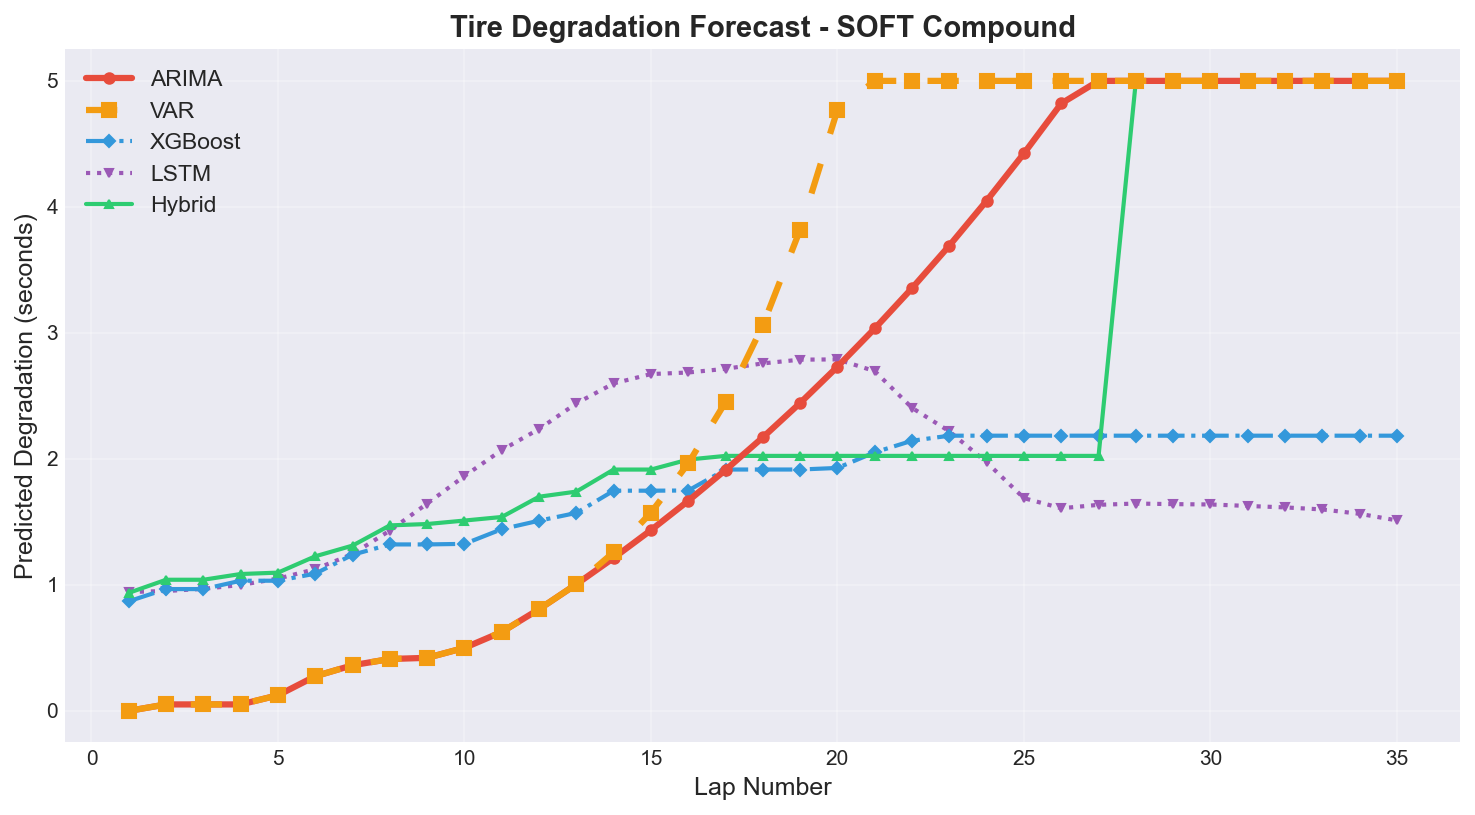
\includegraphics[width=\linewidth]{degradation_curves_soft}
  \caption{SOFT}
\end{subfigure}
\hfill
\begin{subfigure}[b]{0.32\columnwidth}
  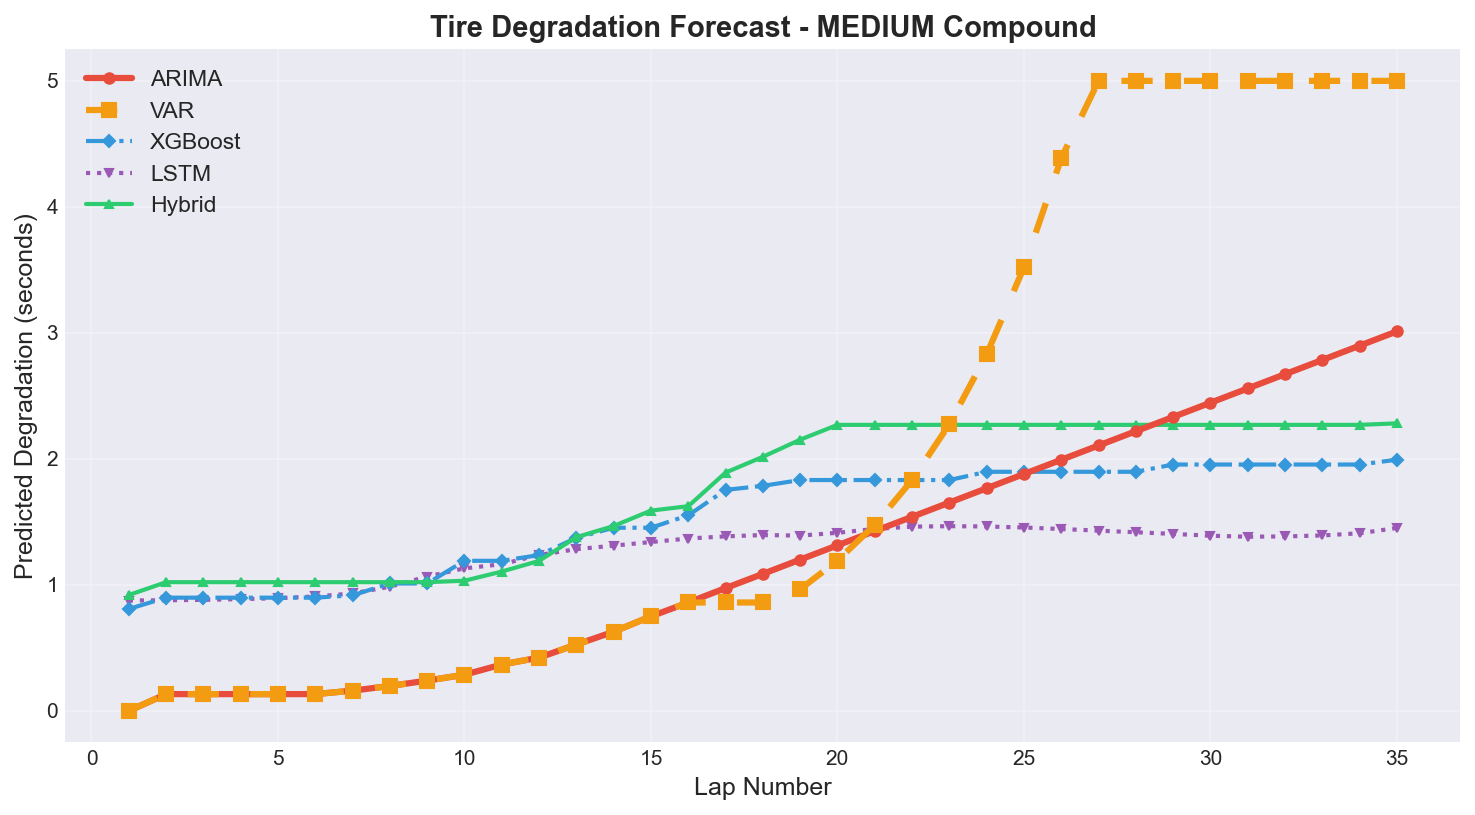
\includegraphics[width=\linewidth]{degradation_curves_medium}
  \caption{MEDIUM}
\end{subfigure}
\hfill
\begin{subfigure}[b]{0.32\columnwidth}
  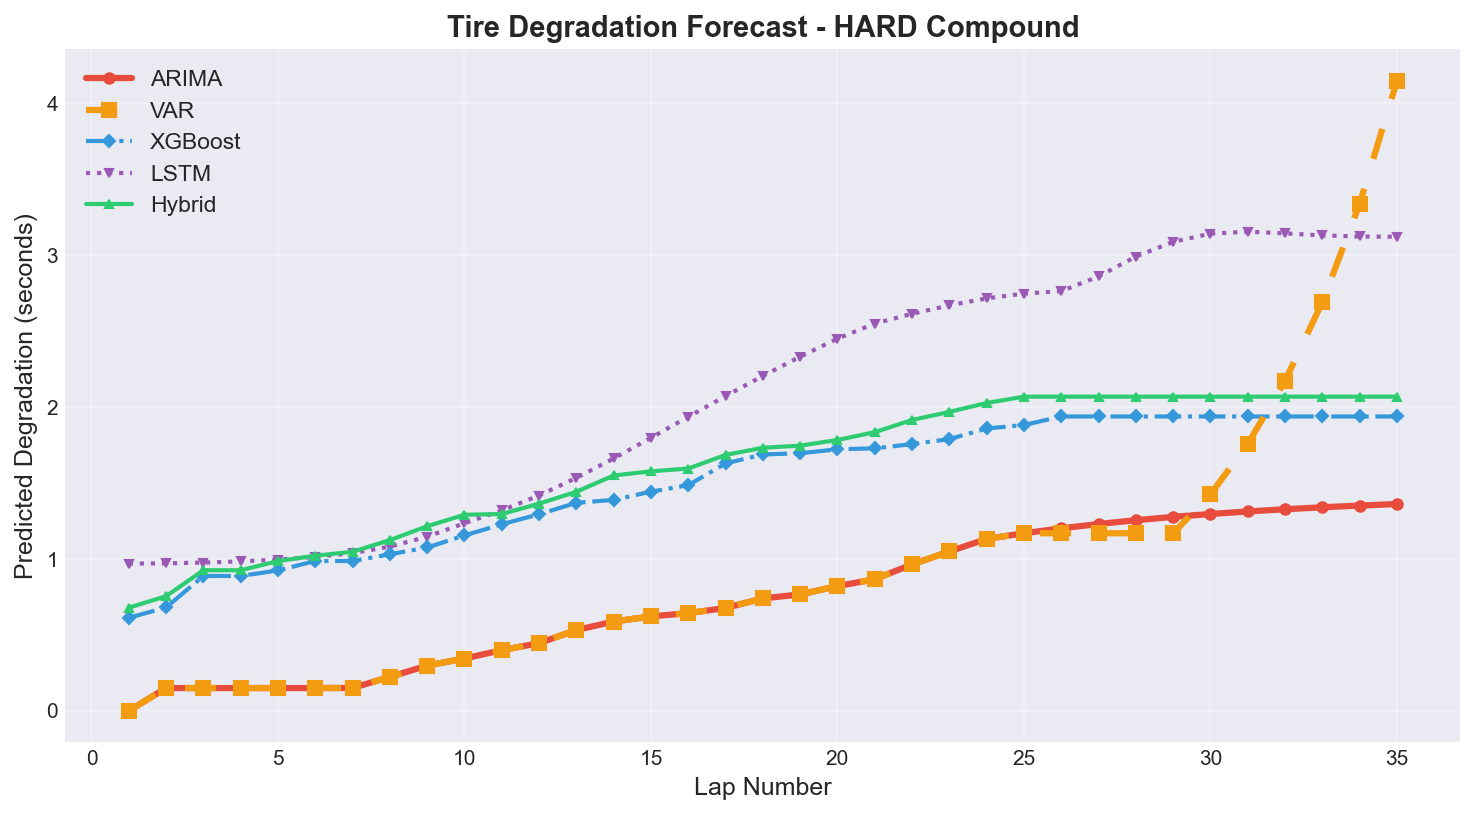
\includegraphics[width=\linewidth]{degradation_curves_hard}
  \caption{HARD}
\end{subfigure}
\caption{Degradation profiles by compound showing mean (solid line) and
inter-stint variance ($\pm 1\sigma$ shaded regions).  SOFT degrades
fastest; HARD is most durable.}
\label{fig:deg_curves}
\end{figure}

% ══════════════════════════════════════════════════════════════════════════
%                         IV. METHODOLOGY
% ══════════════════════════════════════════════════════════════════════════
\section{Methodology}\label{sec:method}

This section details the five modelling approaches employed.  All models
receive identically pre-processed data; time-series models (ARIMA, VAR)
operate on stint-averaged degradation curves, while instance-level
models (XGBoost, LSTM, Hybrid) operate on individual lap rows with
the full 43-feature set.

Fig.~\ref{fig:pipeline} provides an overview of the end-to-end
pipeline.

\begin{figure}[!t]
\centering
\fbox{\parbox{0.95\columnwidth}{\centering
\textbf{End-to-End Pipeline}\\[4pt]
FastF1 API $\rightarrow$
Raw Laps ($\approx$32K) $\rightarrow$
Cleaning (6 stages) $\rightarrow$
22\,401 Clean Laps\\[4pt]
$\rightarrow$ Feature Engineering (43 features) $\rightarrow$\\[4pt]
\{Time-Series Curves (862 stints)\} \& \{Instance Rows (22\,401)\}
$\rightarrow$\\[4pt]
\textbf{Train:} ARIMA $|$ VAR $|$ XGBoost $|$ BiLSTM $|$ Hybrid
$\rightarrow$\\[4pt]
\textbf{Evaluate:} Curve-level \& Instance-level
$\rightarrow$ Strategy Engine $\rightarrow$ Dashboard
}}
\caption{End-to-end data and modelling pipeline from raw telemetry
ingestion through model training to interactive strategy deployment.}
\label{fig:pipeline}
\end{figure}

\subsection{Model~1: ARIMA}\label{sec:arima}

\subsubsection{Motivation and Formulation}

Autoregressive Integrated Moving Average (ARIMA) models are the
classical choice for univariate time-series
forecasting~\cite{box2015time}.  An ARIMA$(p,d,q)$ model is defined as:

\begin{equation}
  \phi(B)(1-B)^d y_t = \theta(B)\varepsilon_t
  \label{eq:arima}
\end{equation}

\noindent where $B$ is the backshift operator ($By_t = y_{t-1}$),
$\phi(B) = 1 - \phi_1 B - \cdots - \phi_p B^p$ is the autoregressive
polynomial of order~$p$, $\theta(B) = 1 + \theta_1 B + \cdots +
\theta_q B^q$ is the moving average polynomial of order~$q$, $d$ is
the differencing order, and $\varepsilon_t \sim \mathcal{N}(0,
\sigma^2)$ is white noise.

We treat each compound's average degradation curve as a short time
series ($T \approx 20$--40 observations, depending on the compound's
typical stint length) and fit a separate ARIMA model per compound.

\subsubsection{Stationarity Testing}\label{sec:stationarity}

A prerequisite for ARIMA modelling is that the time series be stationary
(or rendered stationary through differencing).  We employ a two-test
approach:

\begin{enumerate}
  \item \textbf{Augmented Dickey--Fuller (ADF):}  Tests the null
  hypothesis of a unit root.  If $p < 0.05$, the series is deemed
  stationary.  Maximum lag is set to $\lfloor\sqrt{n}\rfloor$ to ensure
  sufficient effective observations on short curves.

  \item \textbf{KPSS:}  Tests the null hypothesis of stationarity.  If
  the ADF test is inconclusive (which occurs frequently with short
  series), KPSS provides a confirmatory check: if KPSS fails to reject
  stationarity ($p > 0.05$), the series is accepted as stationary.
\end{enumerate}

The differencing order $d$ is determined iteratively: starting from
$d=0$, the series is differenced until both tests agree on
stationarity, up to a maximum of $d=2$.

\subsubsection{Order Selection}

For each compound, after determining $d$, a grid search is performed
over $p \in \{0, 1, 2, 3\}$ and $q \in \{0, 1, 2, 3\}$ (excluding
$p=q=0$), selecting the $(p,q)$ pair that minimises the Akaike
Information Criterion (AIC):

\begin{equation}
  \text{AIC} = 2k - 2\ln(\hat{L})
  \label{eq:aic}
\end{equation}

\noindent where $k$ is the number of estimated parameters and $\hat{L}$
is the maximum value of the likelihood function.

The selected orders are shown in Table~\ref{tab:arima_orders}.

\begin{table}[!t]
\caption{ARIMA Model Orders Selected by AIC Grid Search}
\label{tab:arima_orders}
\centering
\footnotesize
\begin{tabular}{@{}lcccc@{}}
\toprule
\textbf{Compound} & \textbf{$p$} & \textbf{$d$} & \textbf{$q$} & \textbf{AIC} \\
\midrule
HARD   & 1 & 1 & 0 & $-91.92$ \\
MEDIUM & 1 & 2 & 0 & $-55.51$ \\
SOFT   & 1 & 0 & 0 & $-26.13$ \\
\bottomrule
\end{tabular}
\end{table}

Notable findings: (i)~SOFT requires no differencing ($d=0$), consistent
with its shorter series length and steeper, more overtly non-stationary
degradation that the AR term alone can capture; (ii)~MEDIUM requires
second-order differencing ($d=2$), suggesting a more complex trend
structure; (iii)~all compounds select $p=1$ and $q=0$, indicating
that a single autoregressive lag captures the temporal dynamics
without requiring moving-average terms.

\subsubsection{Diagnostics}

Fig.~\ref{fig:arima_stationarity} shows the stationarity test
visualisations for each compound, confirming that the raw degradation
series are non-stationary in levels (as expected---degradation
increases monotonically with tyre life) and become stationary after the
selected differencing.  Fig.~\ref{fig:arima_acf_pacf} presents the
ACF and PACF plots after differencing, validating the lag structure.
Fig.~\ref{fig:arima_residuals} shows residual diagnostics including
the time-series residual plot, histogram, and autocorrelation function,
confirming that residuals are approximately white noise.

\begin{figure}[!t]
\centering
\begin{subfigure}[b]{0.32\columnwidth}
  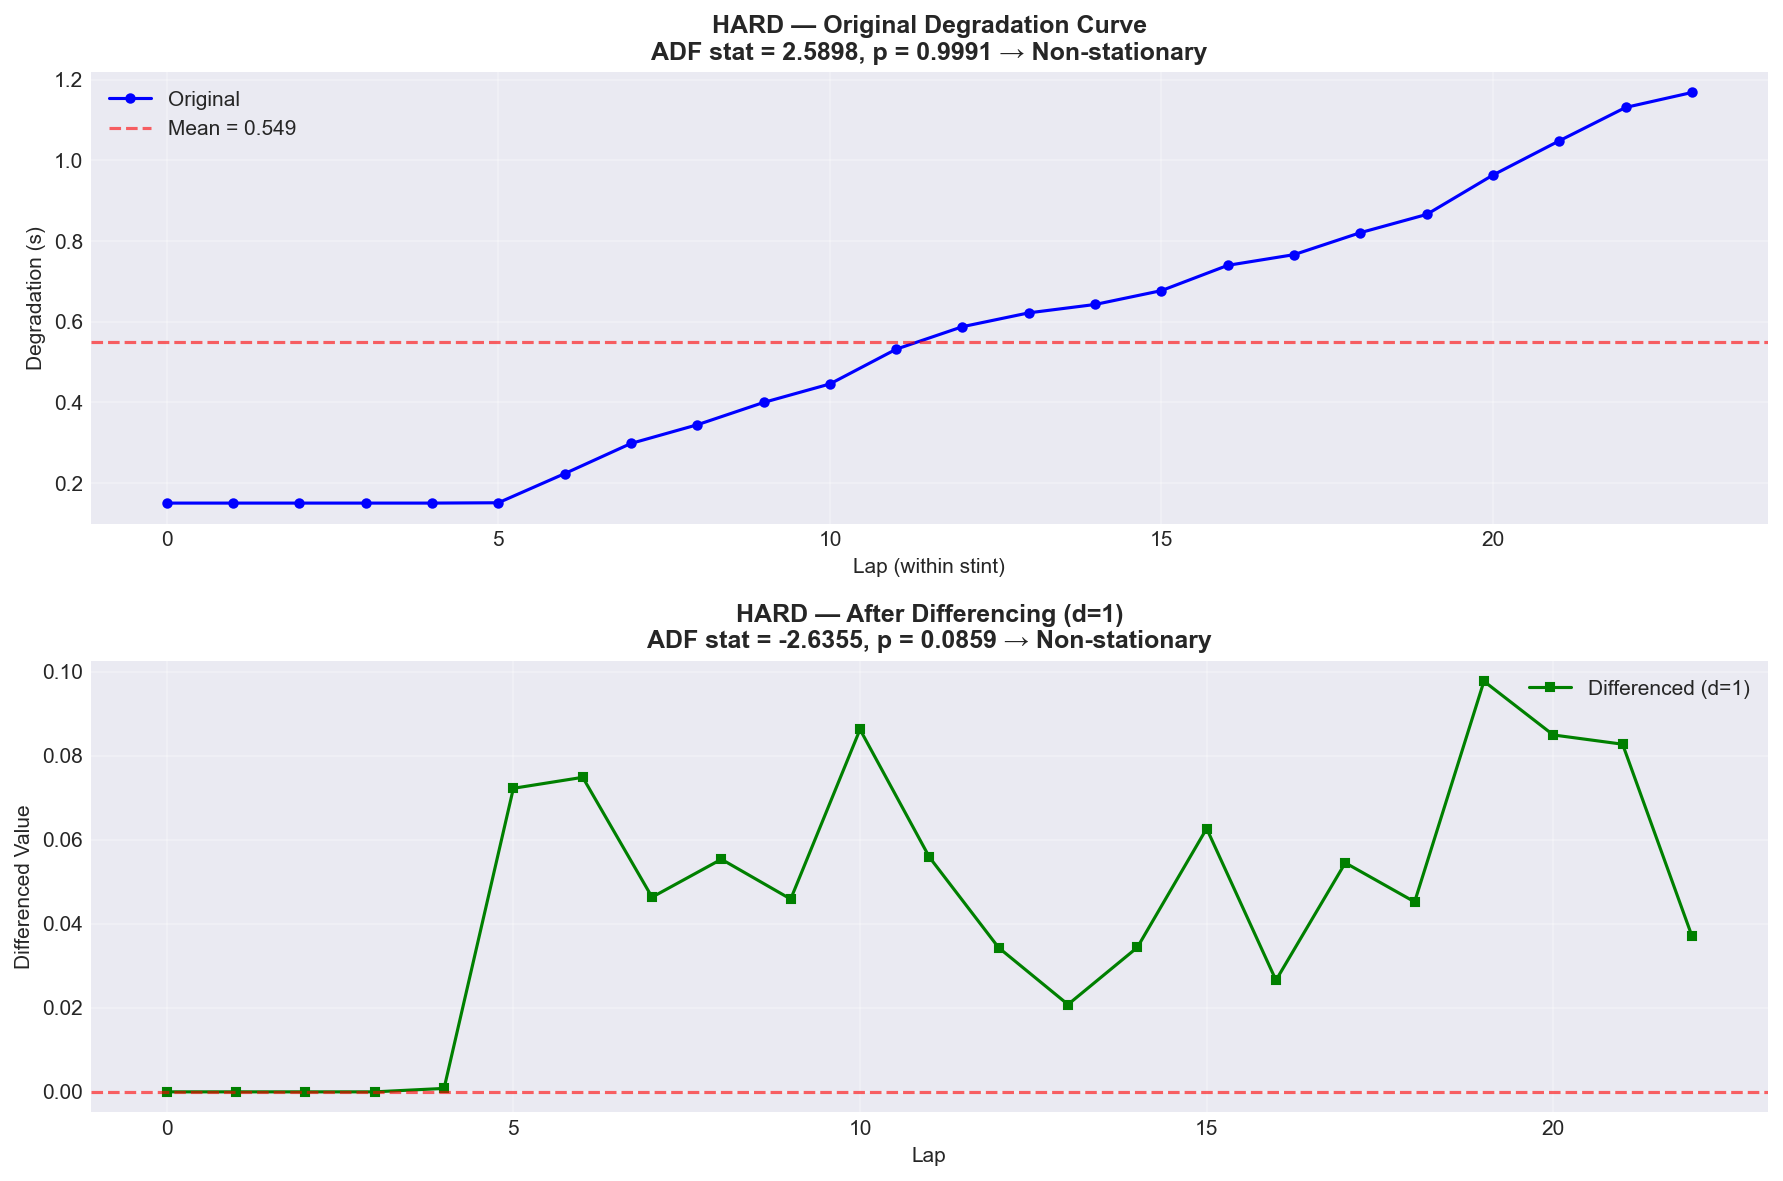
\includegraphics[width=\linewidth]{arima_diagnostics/stationarity_hard}
  \caption{HARD}
\end{subfigure}
\hfill
\begin{subfigure}[b]{0.32\columnwidth}
  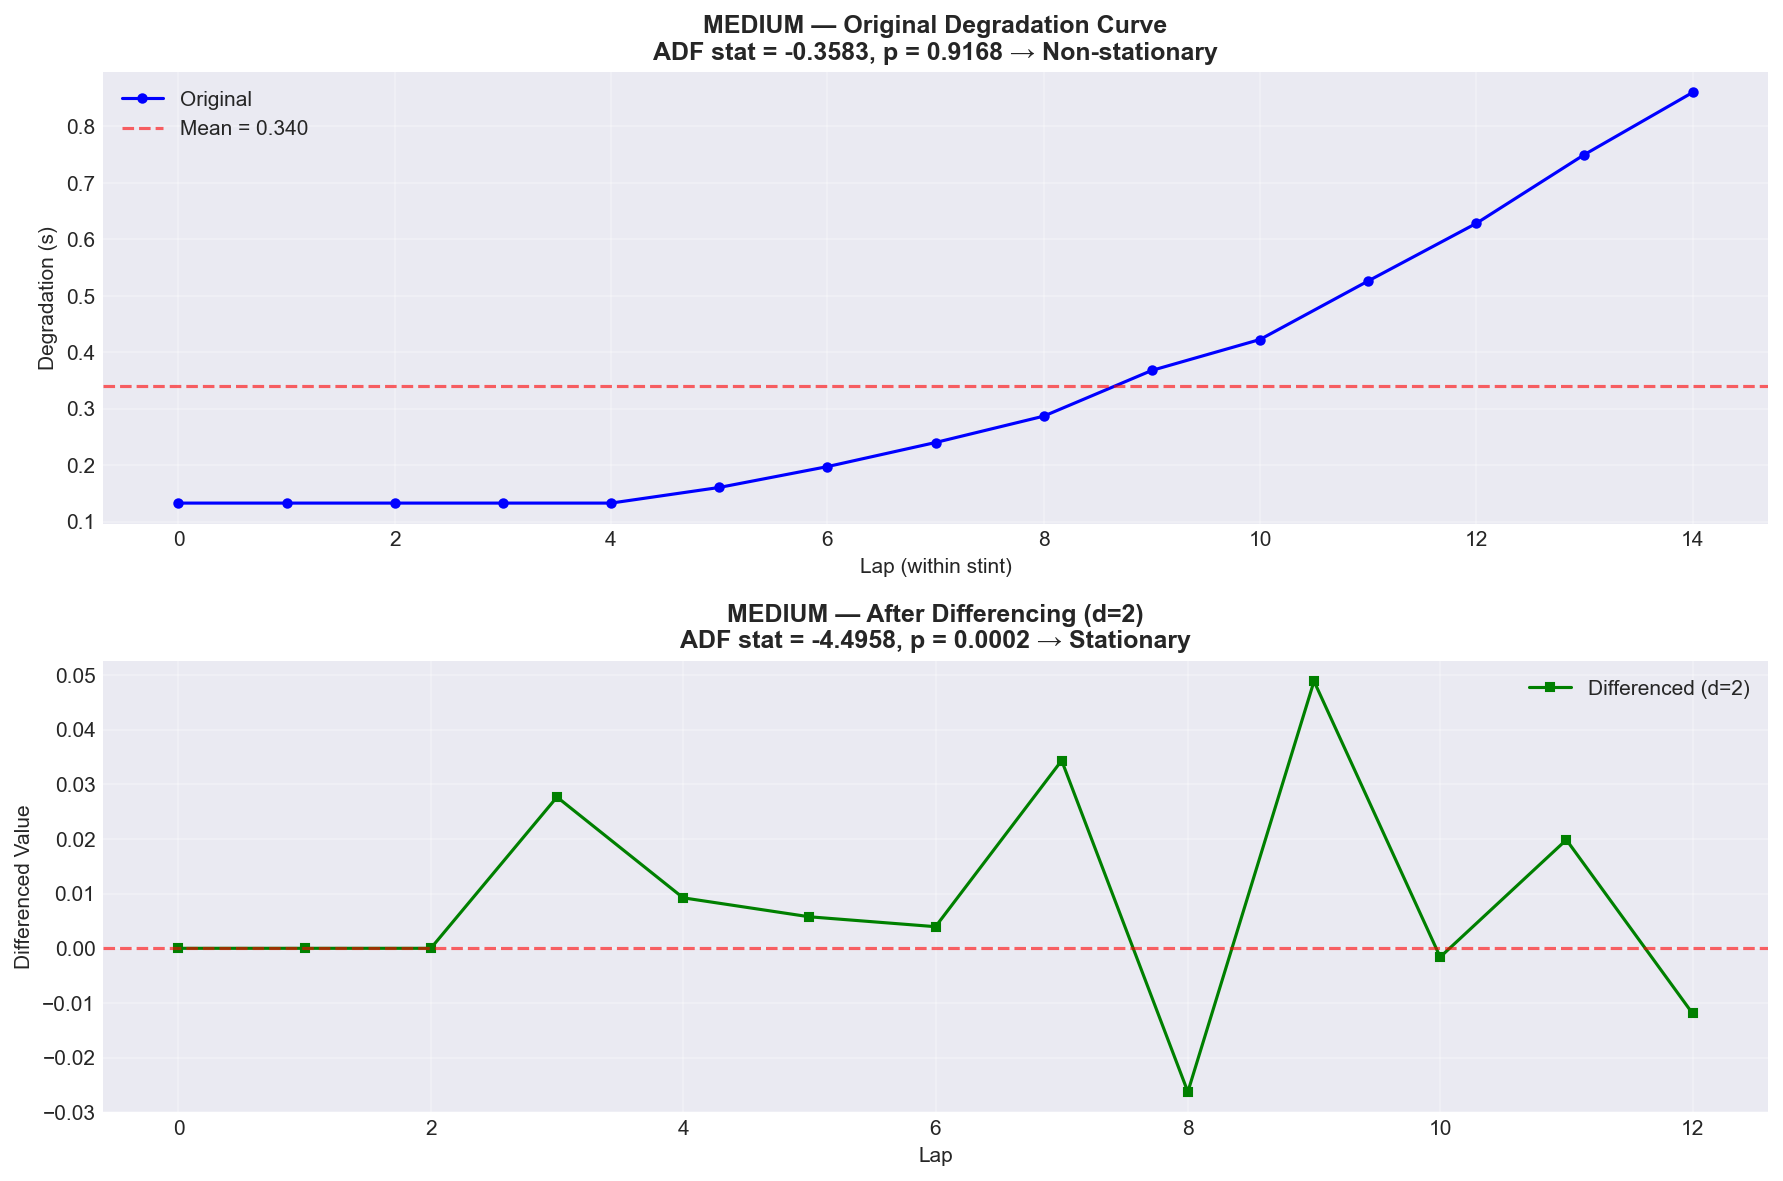
\includegraphics[width=\linewidth]{arima_diagnostics/stationarity_medium}
  \caption{MEDIUM}
\end{subfigure}
\hfill
\begin{subfigure}[b]{0.32\columnwidth}
  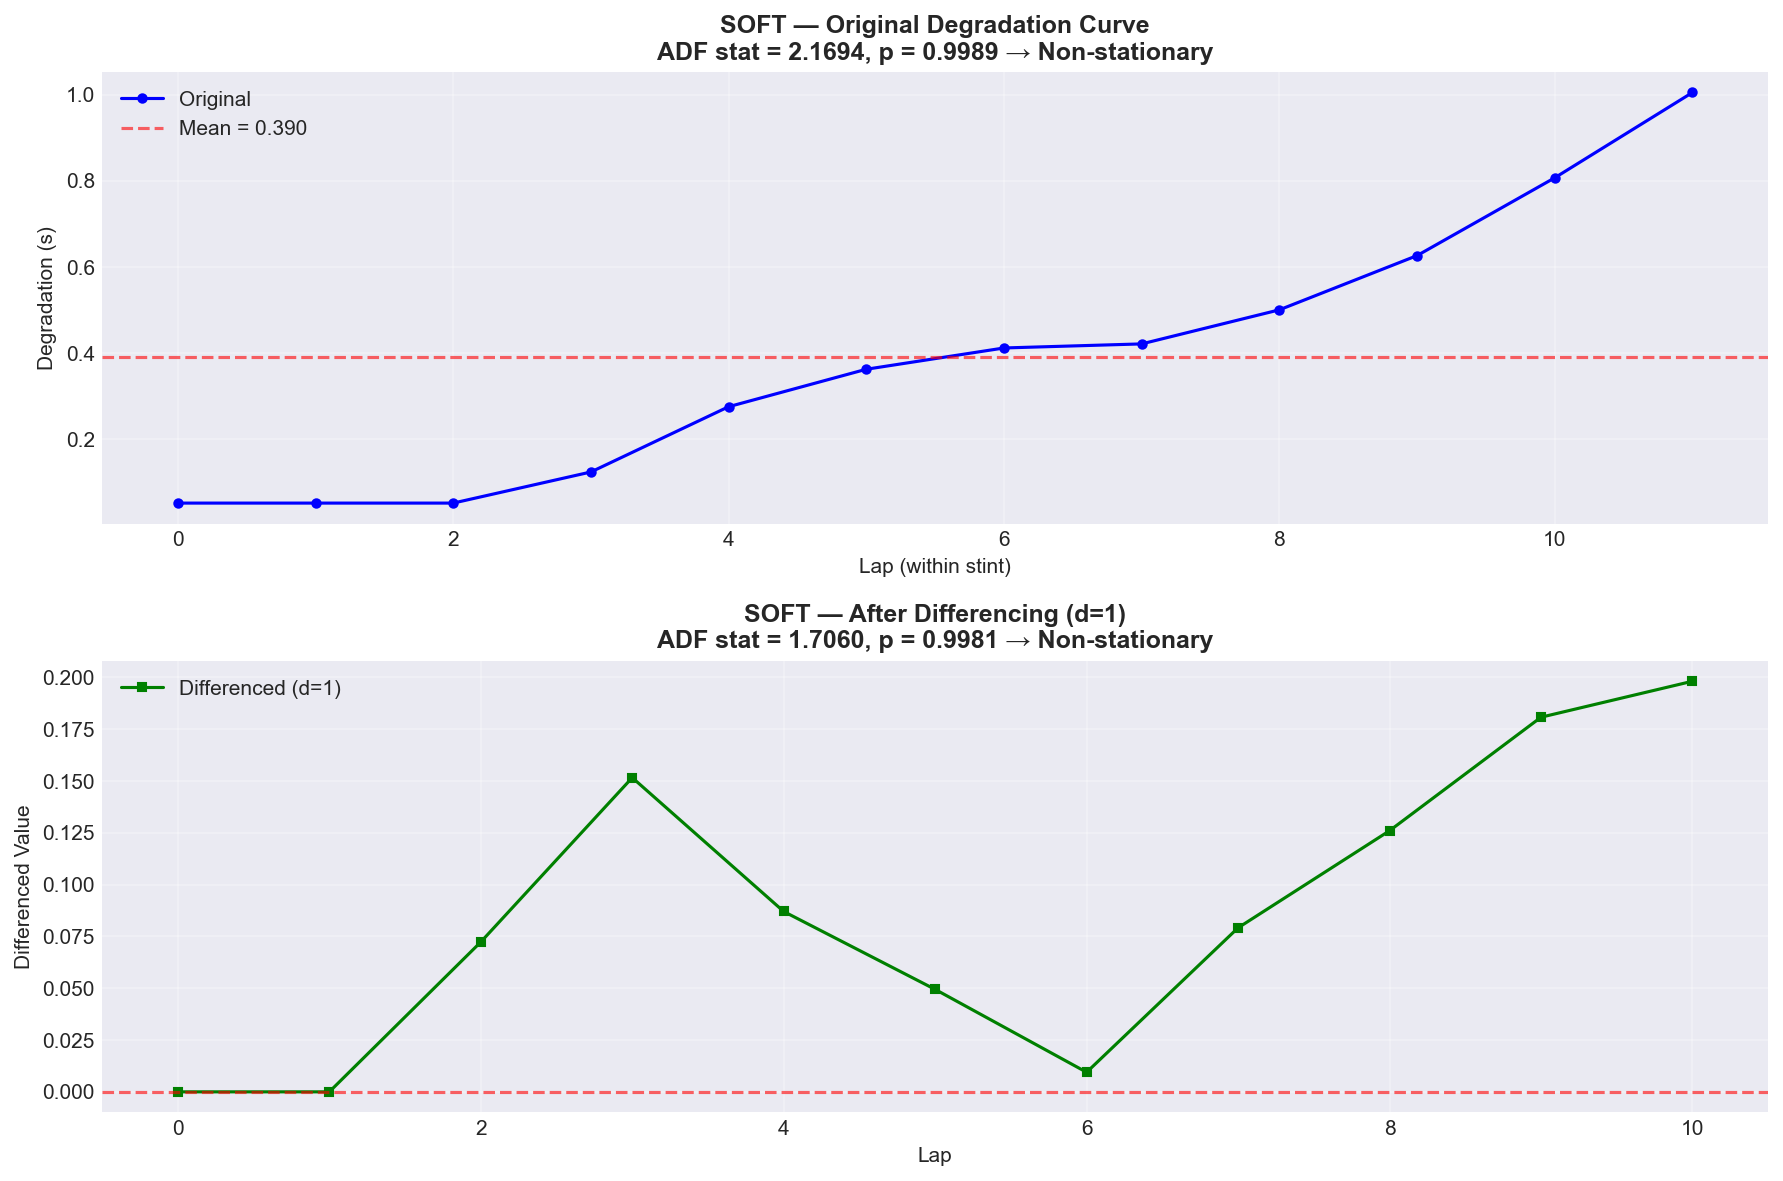
\includegraphics[width=\linewidth]{arima_diagnostics/stationarity_soft}
  \caption{SOFT}
\end{subfigure}
\caption{ARIMA stationarity analysis per compound.  ADF and KPSS
statistics are annotated.  All series are non-stationary in levels and
stationary after the selected differencing order~$d$.}
\label{fig:arima_stationarity}
\end{figure}

\begin{figure}[!t]
\centering
\begin{subfigure}[b]{0.32\columnwidth}
  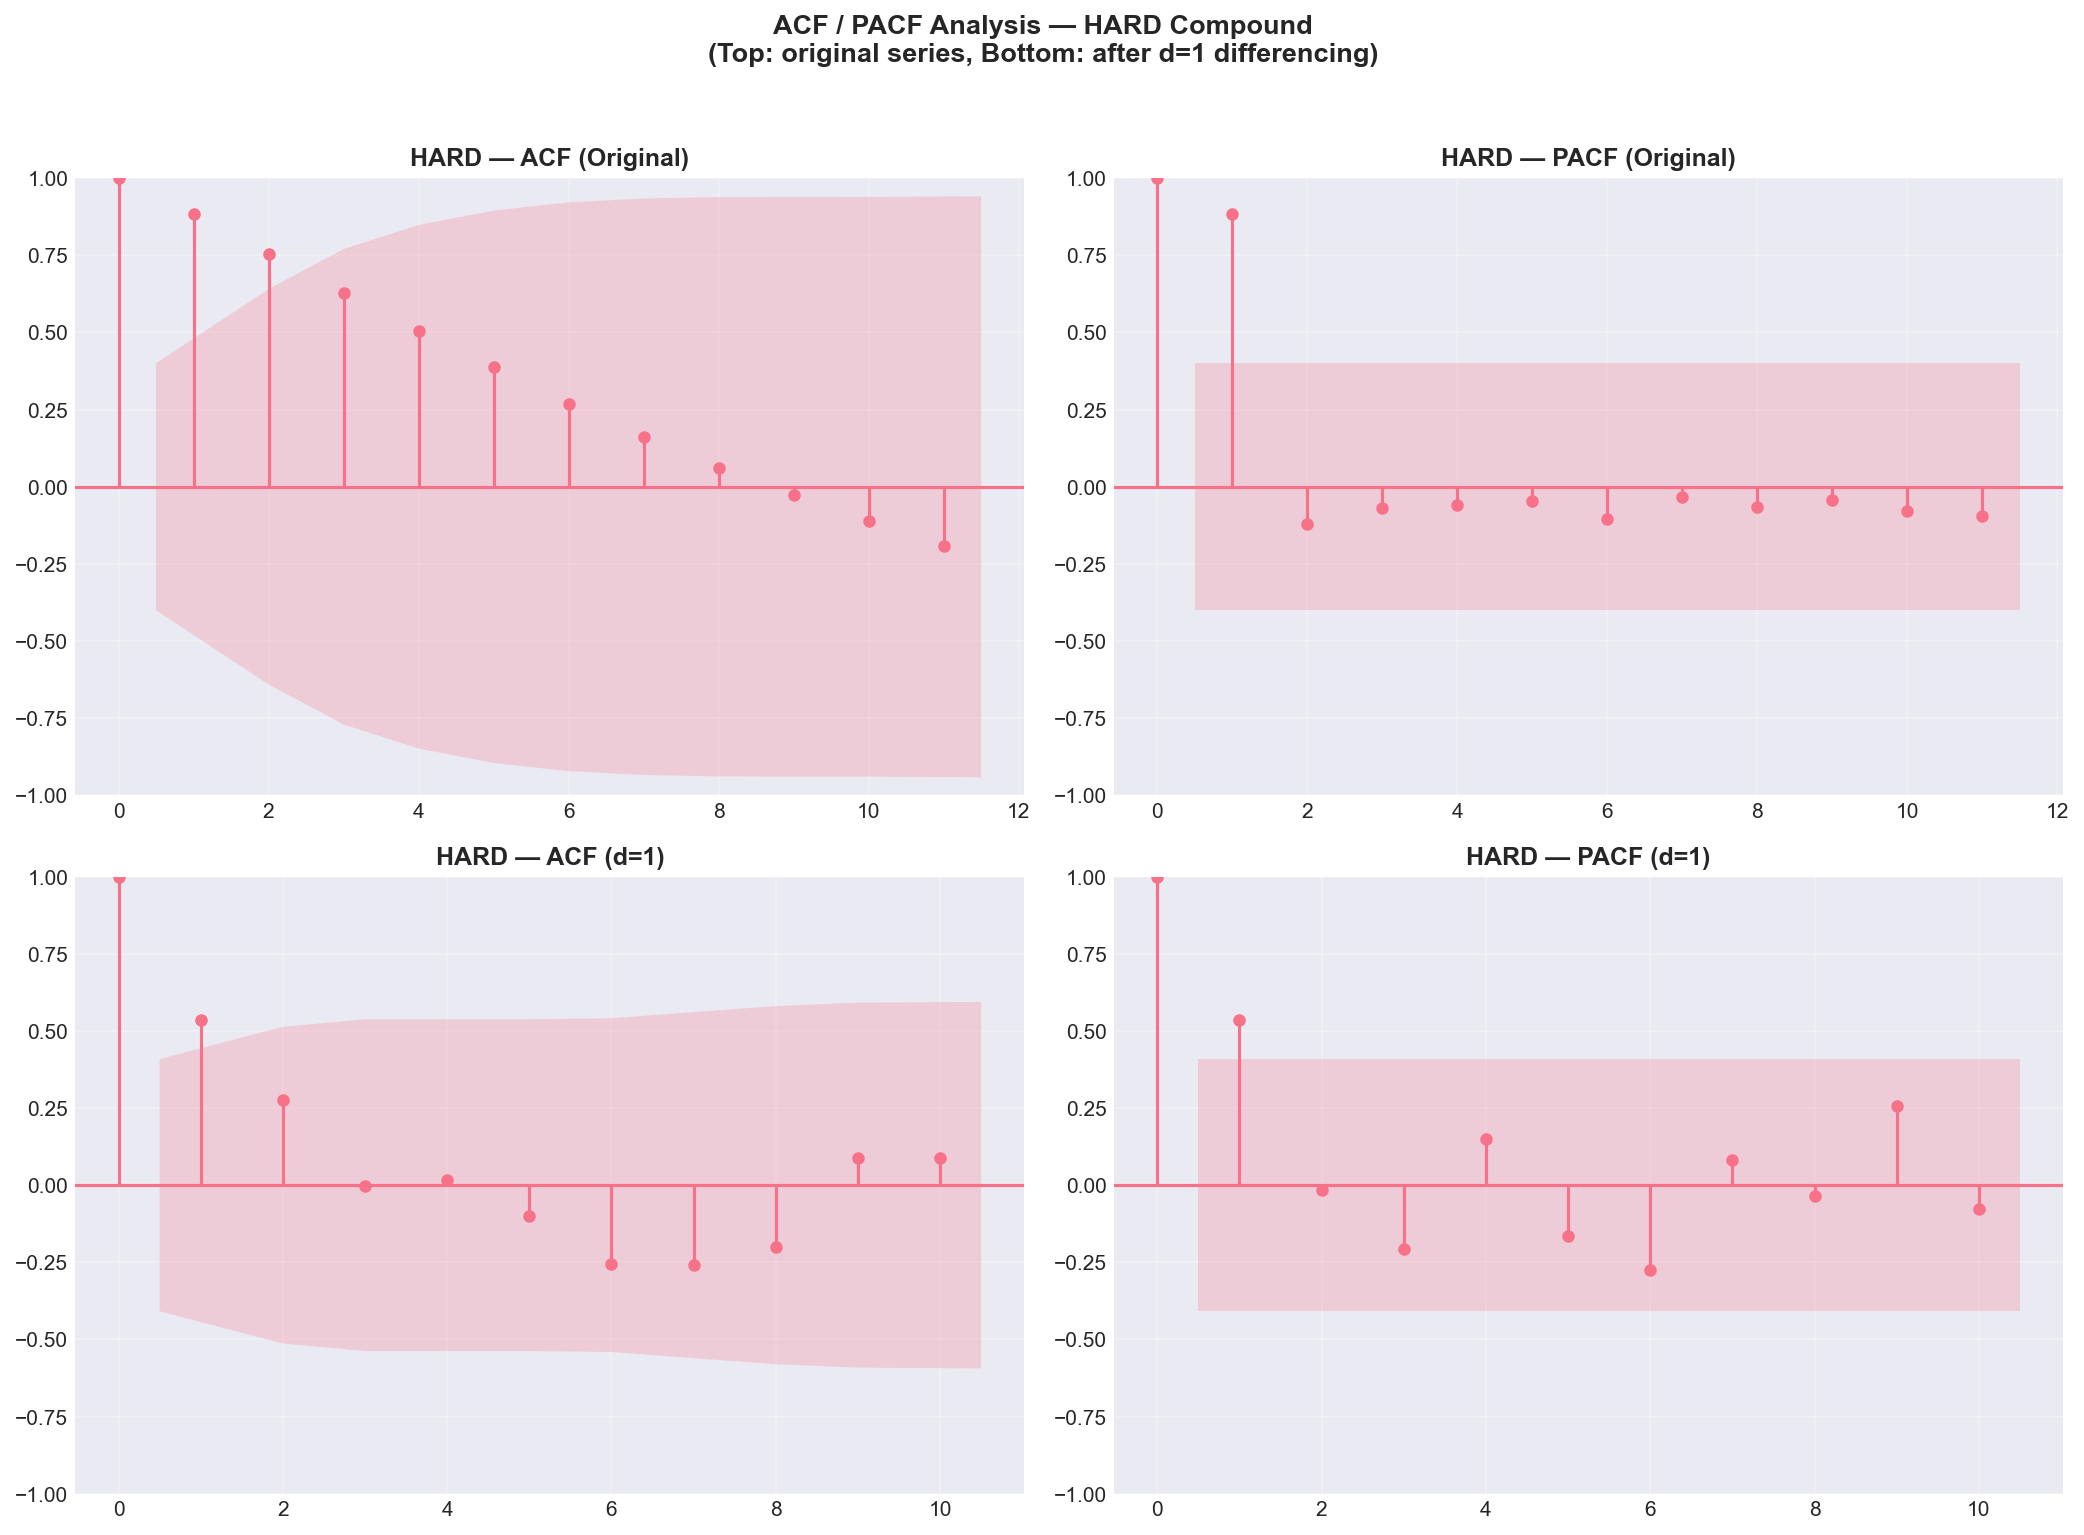
\includegraphics[width=\linewidth]{arima_diagnostics/acf_pacf_hard}
  \caption{HARD}
\end{subfigure}
\hfill
\begin{subfigure}[b]{0.32\columnwidth}
  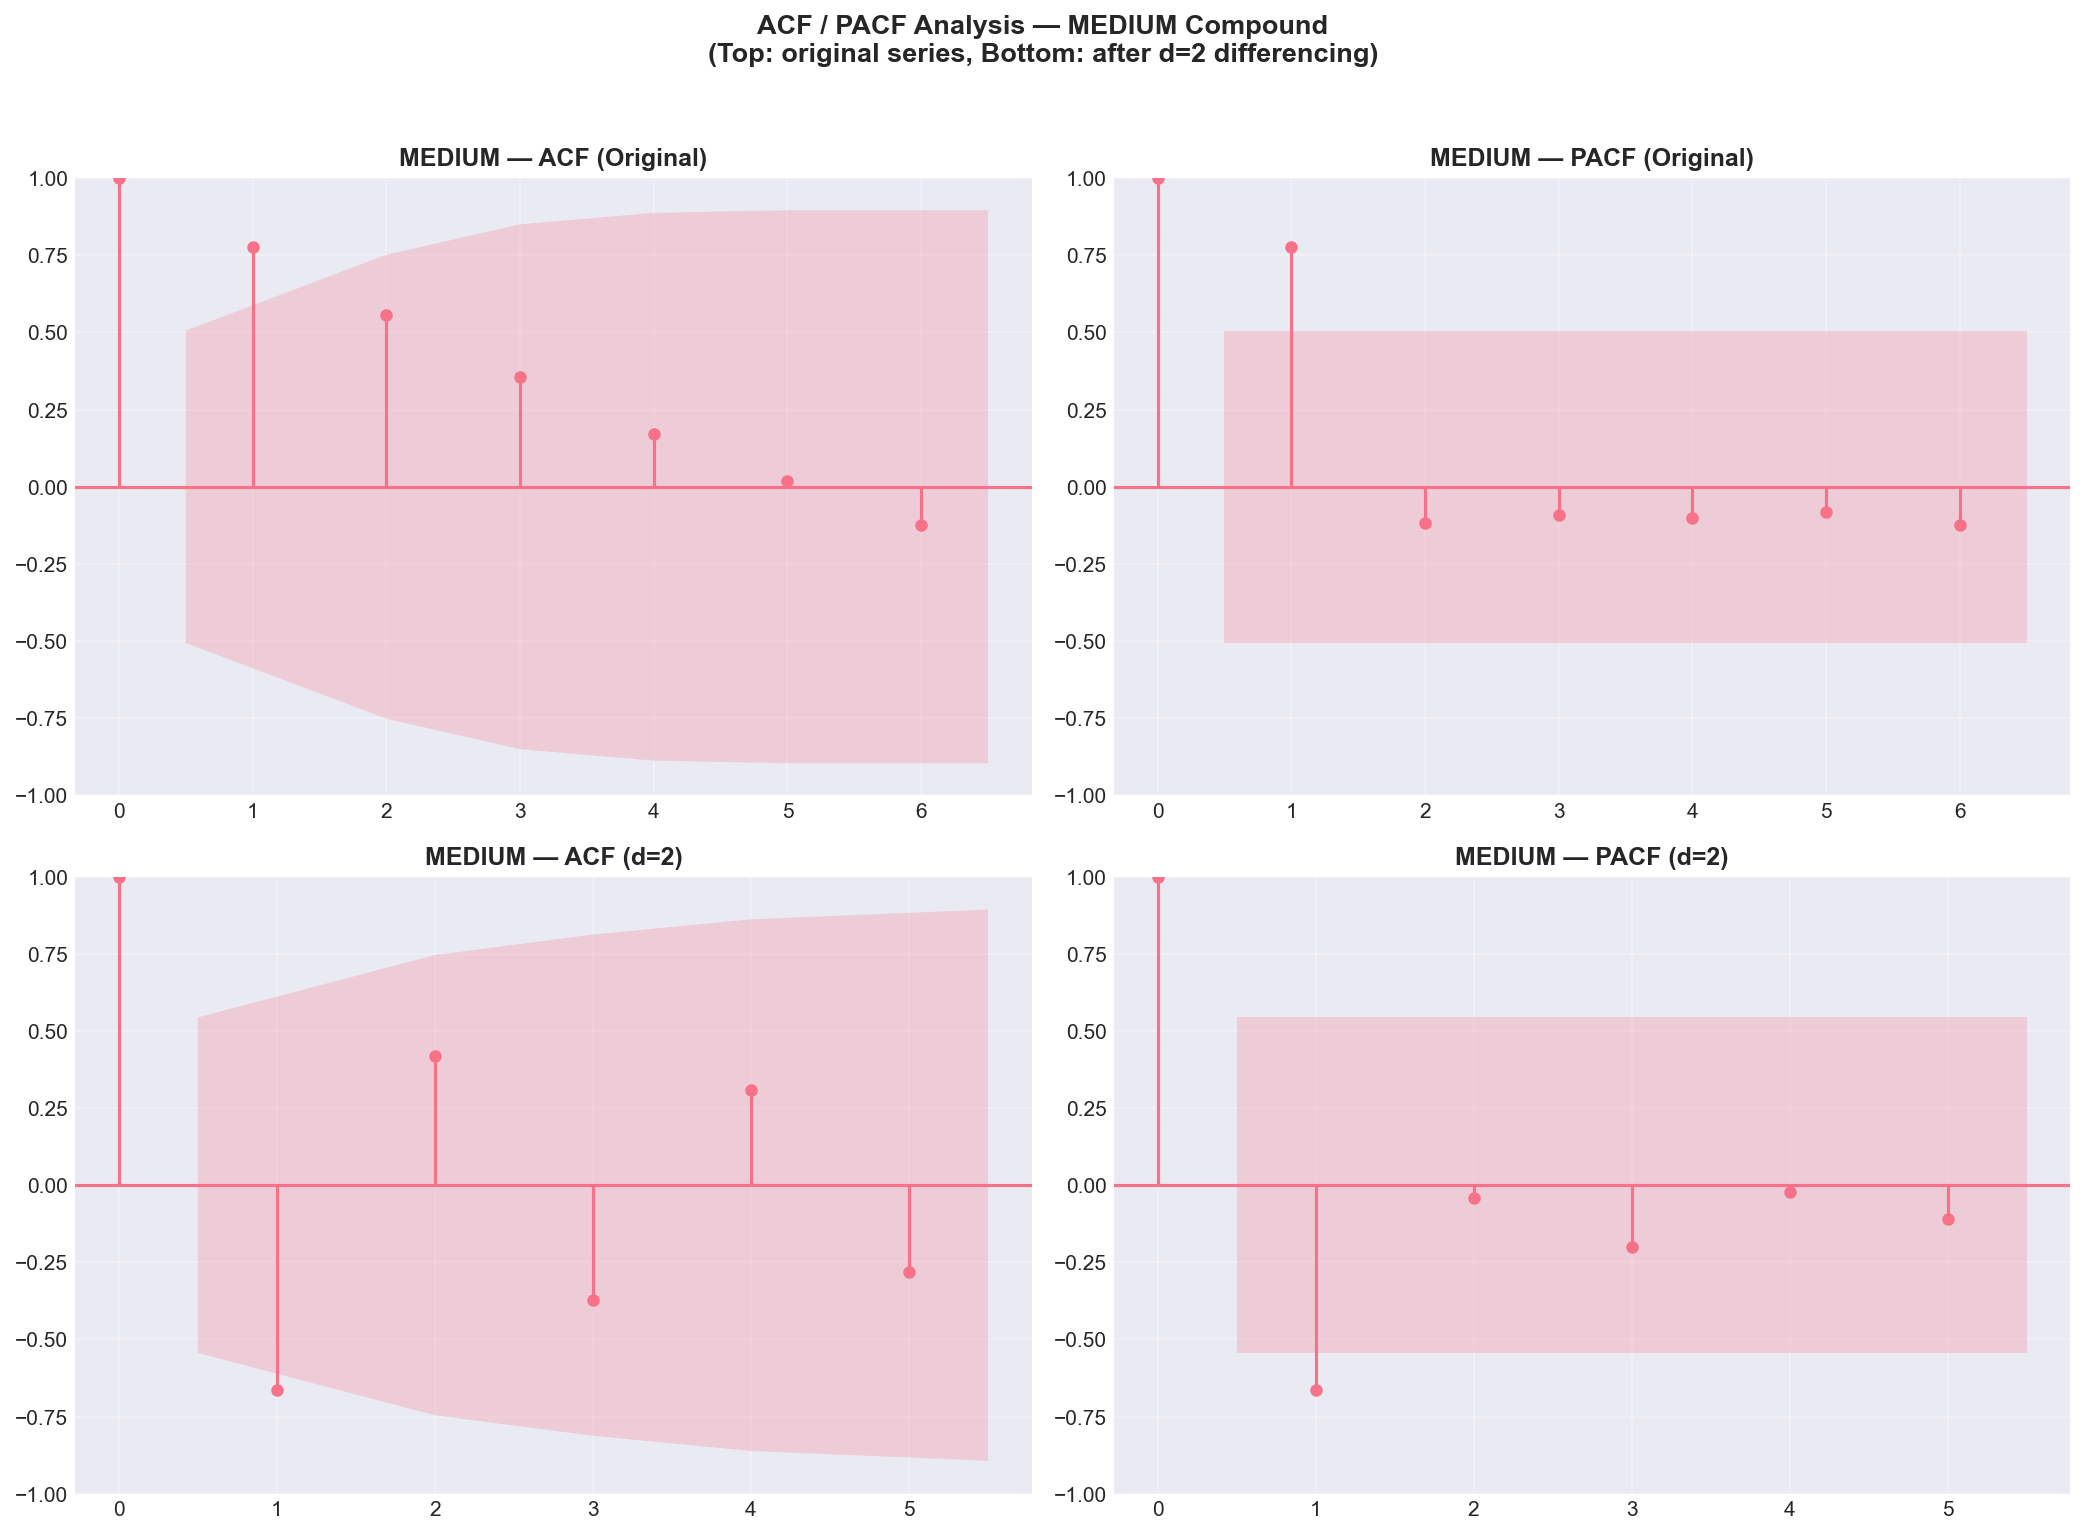
\includegraphics[width=\linewidth]{arima_diagnostics/acf_pacf_medium}
  \caption{MEDIUM}
\end{subfigure}
\hfill
\begin{subfigure}[b]{0.32\columnwidth}
  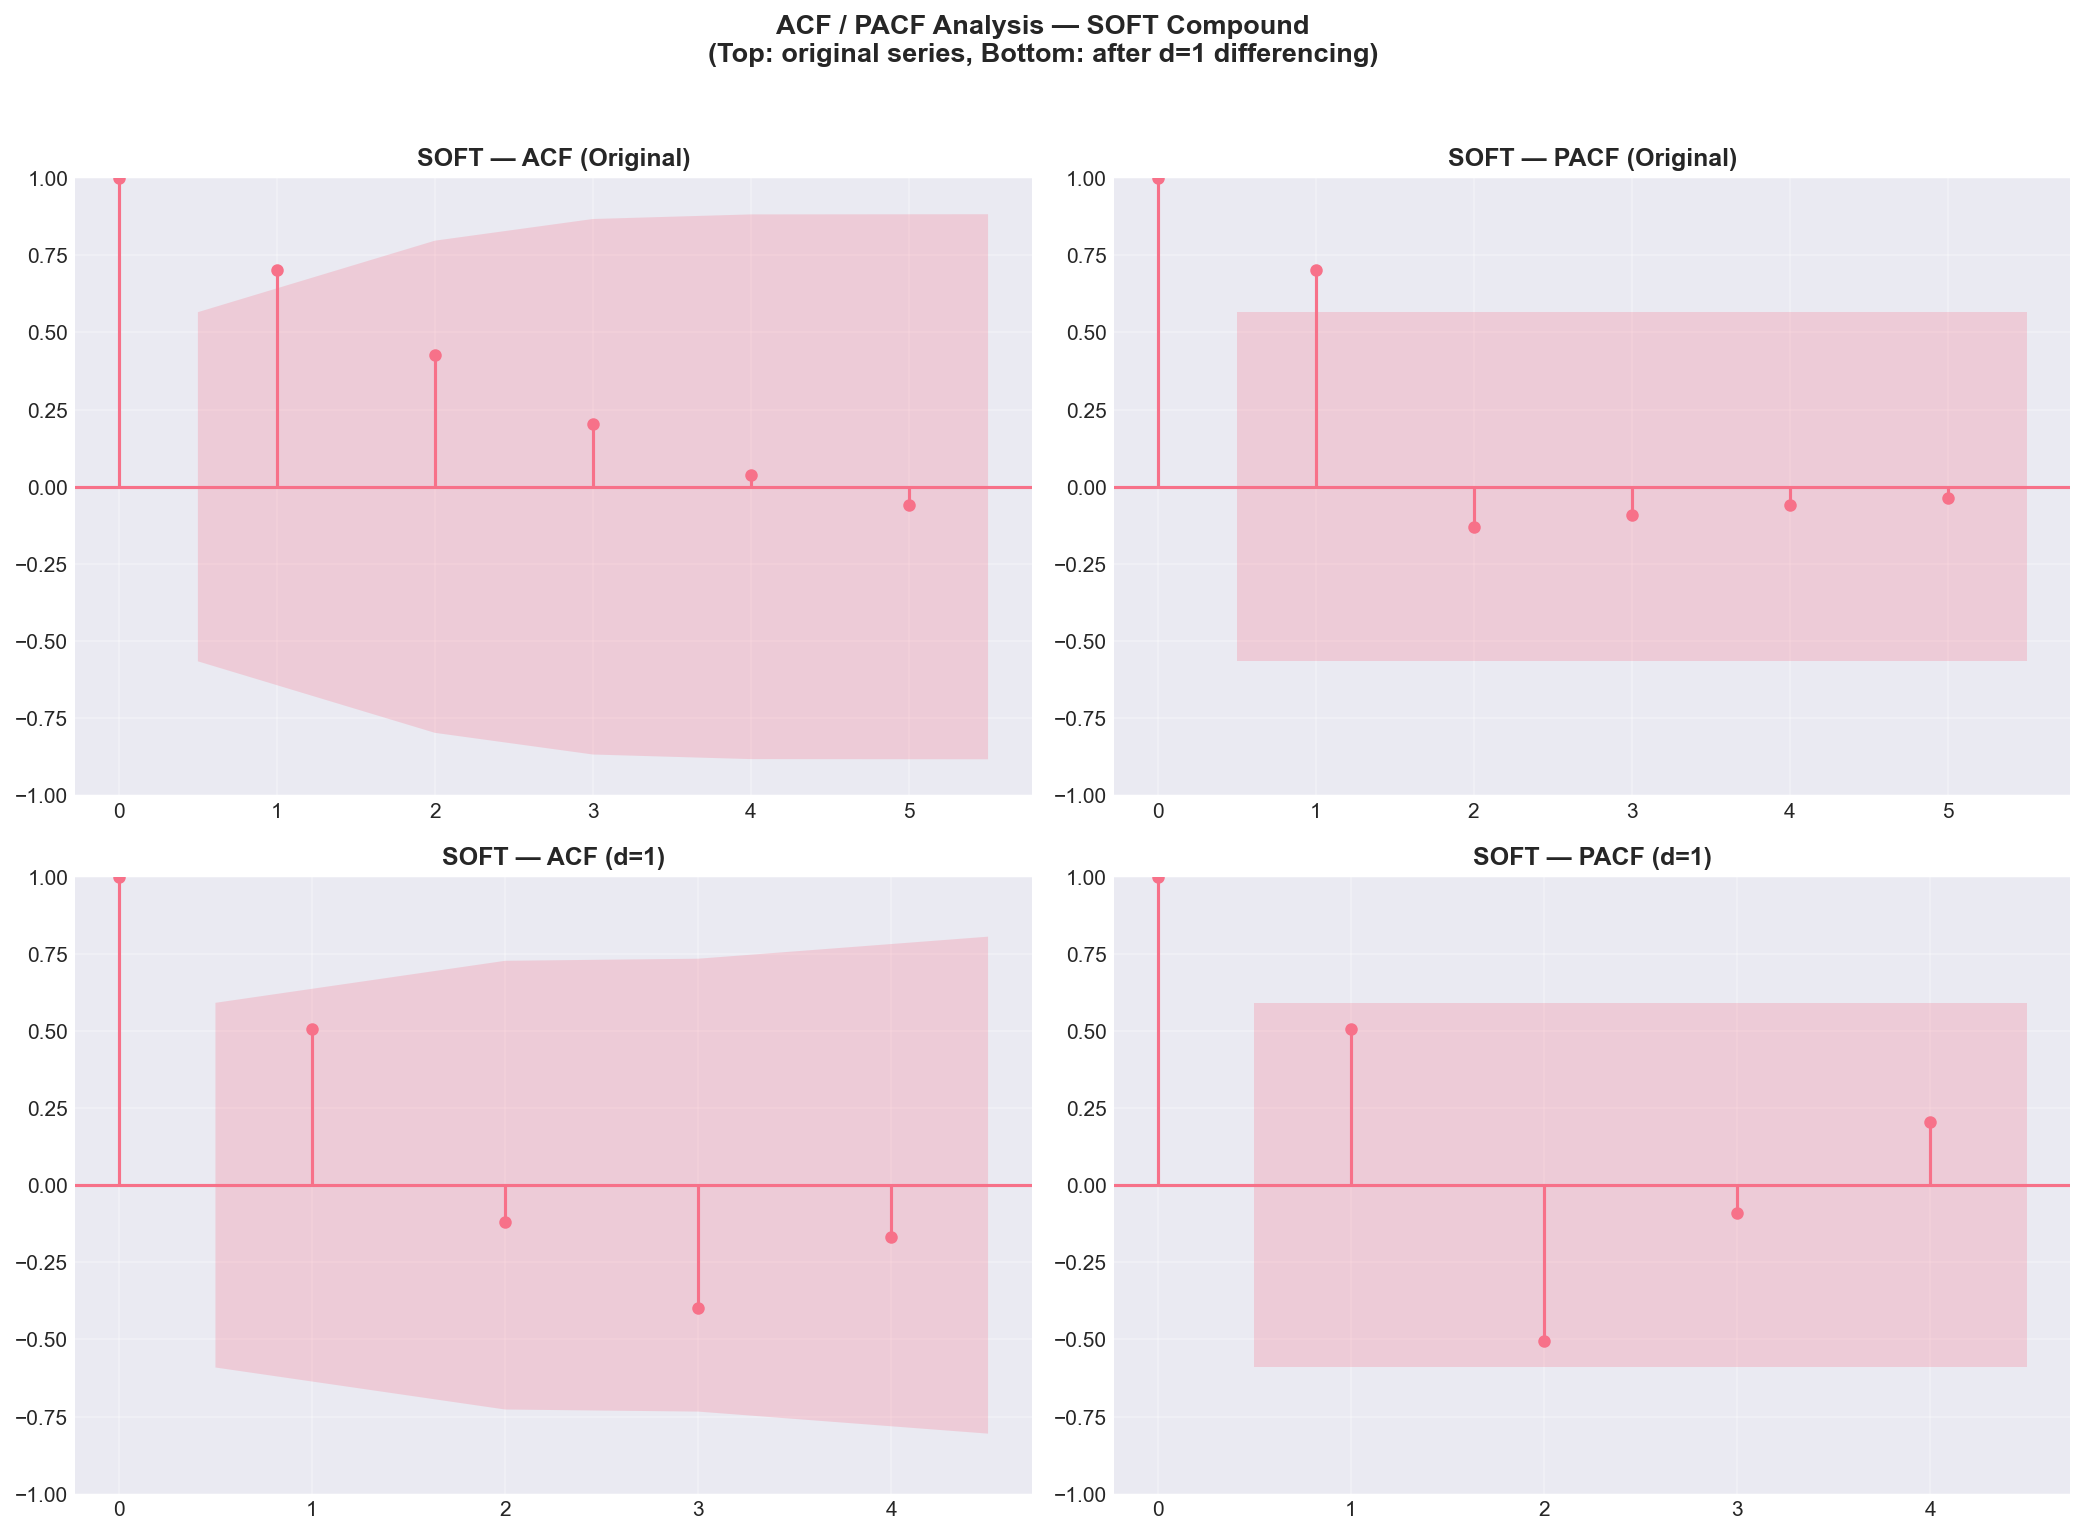
\includegraphics[width=\linewidth]{arima_diagnostics/acf_pacf_soft}
  \caption{SOFT}
\end{subfigure}
\caption{ACF and PACF plots after differencing.  Significant lags
validate the ARIMA order selection.  PACF cuts off after lag~1 for
all compounds, confirming the AR(1) structure.}
\label{fig:arima_acf_pacf}
\end{figure}

\begin{figure}[!t]
\centering
\begin{subfigure}[b]{0.32\columnwidth}
  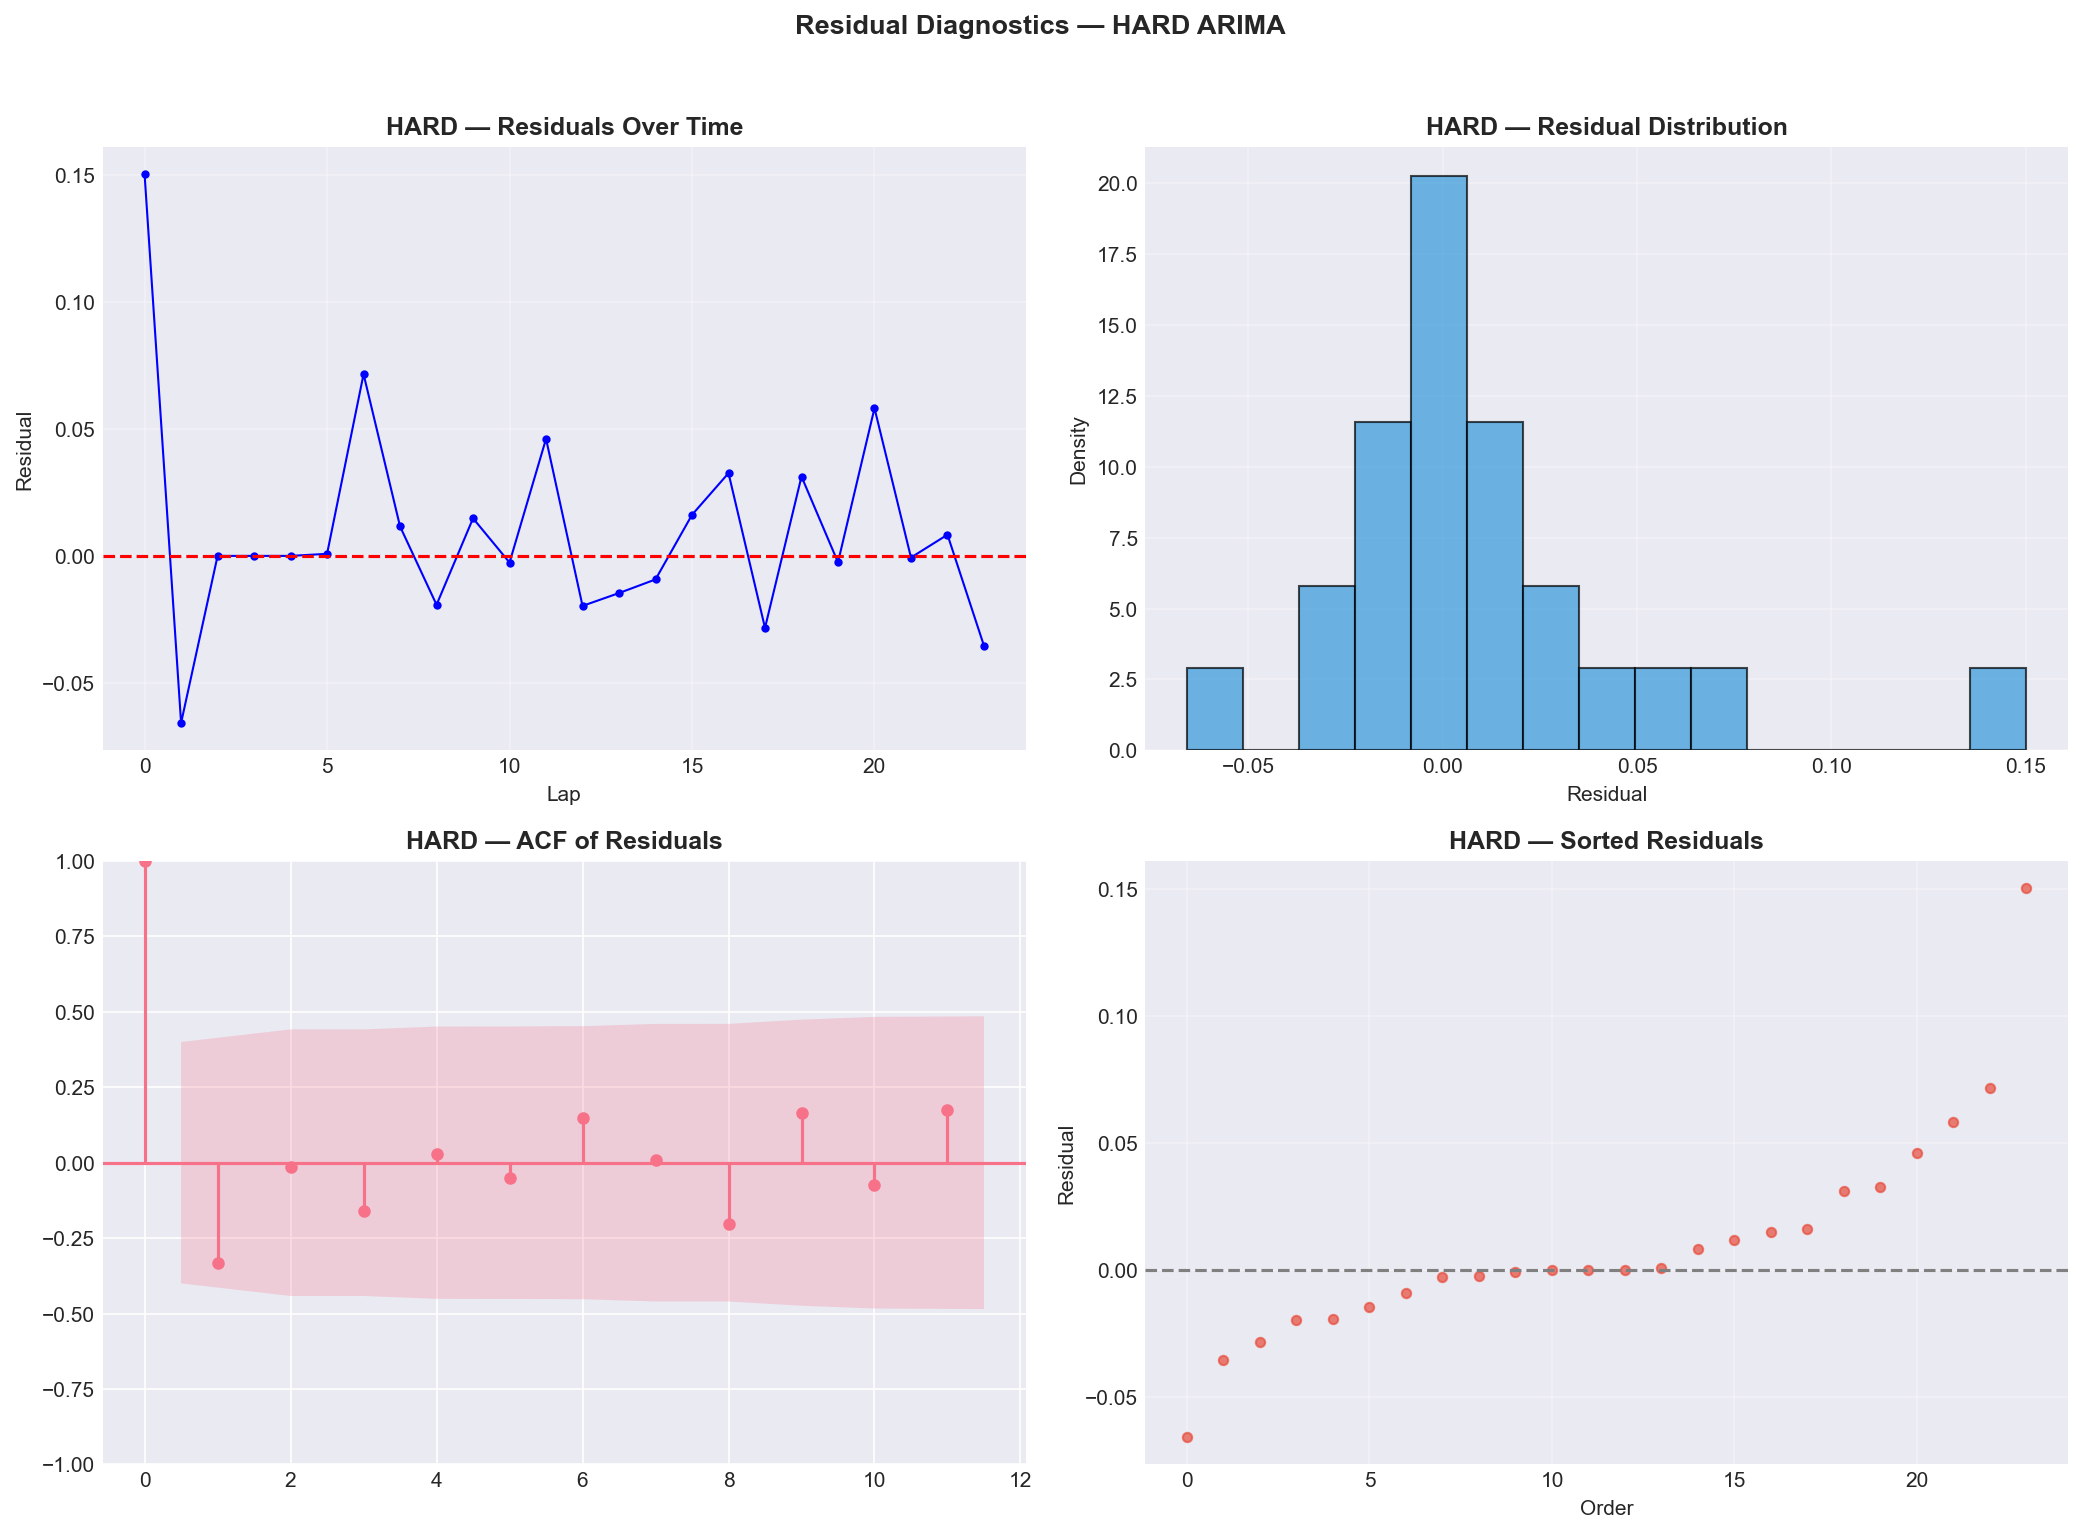
\includegraphics[width=\linewidth]{arima_diagnostics/residuals_hard}
  \caption{HARD}
\end{subfigure}
\hfill
\begin{subfigure}[b]{0.32\columnwidth}
  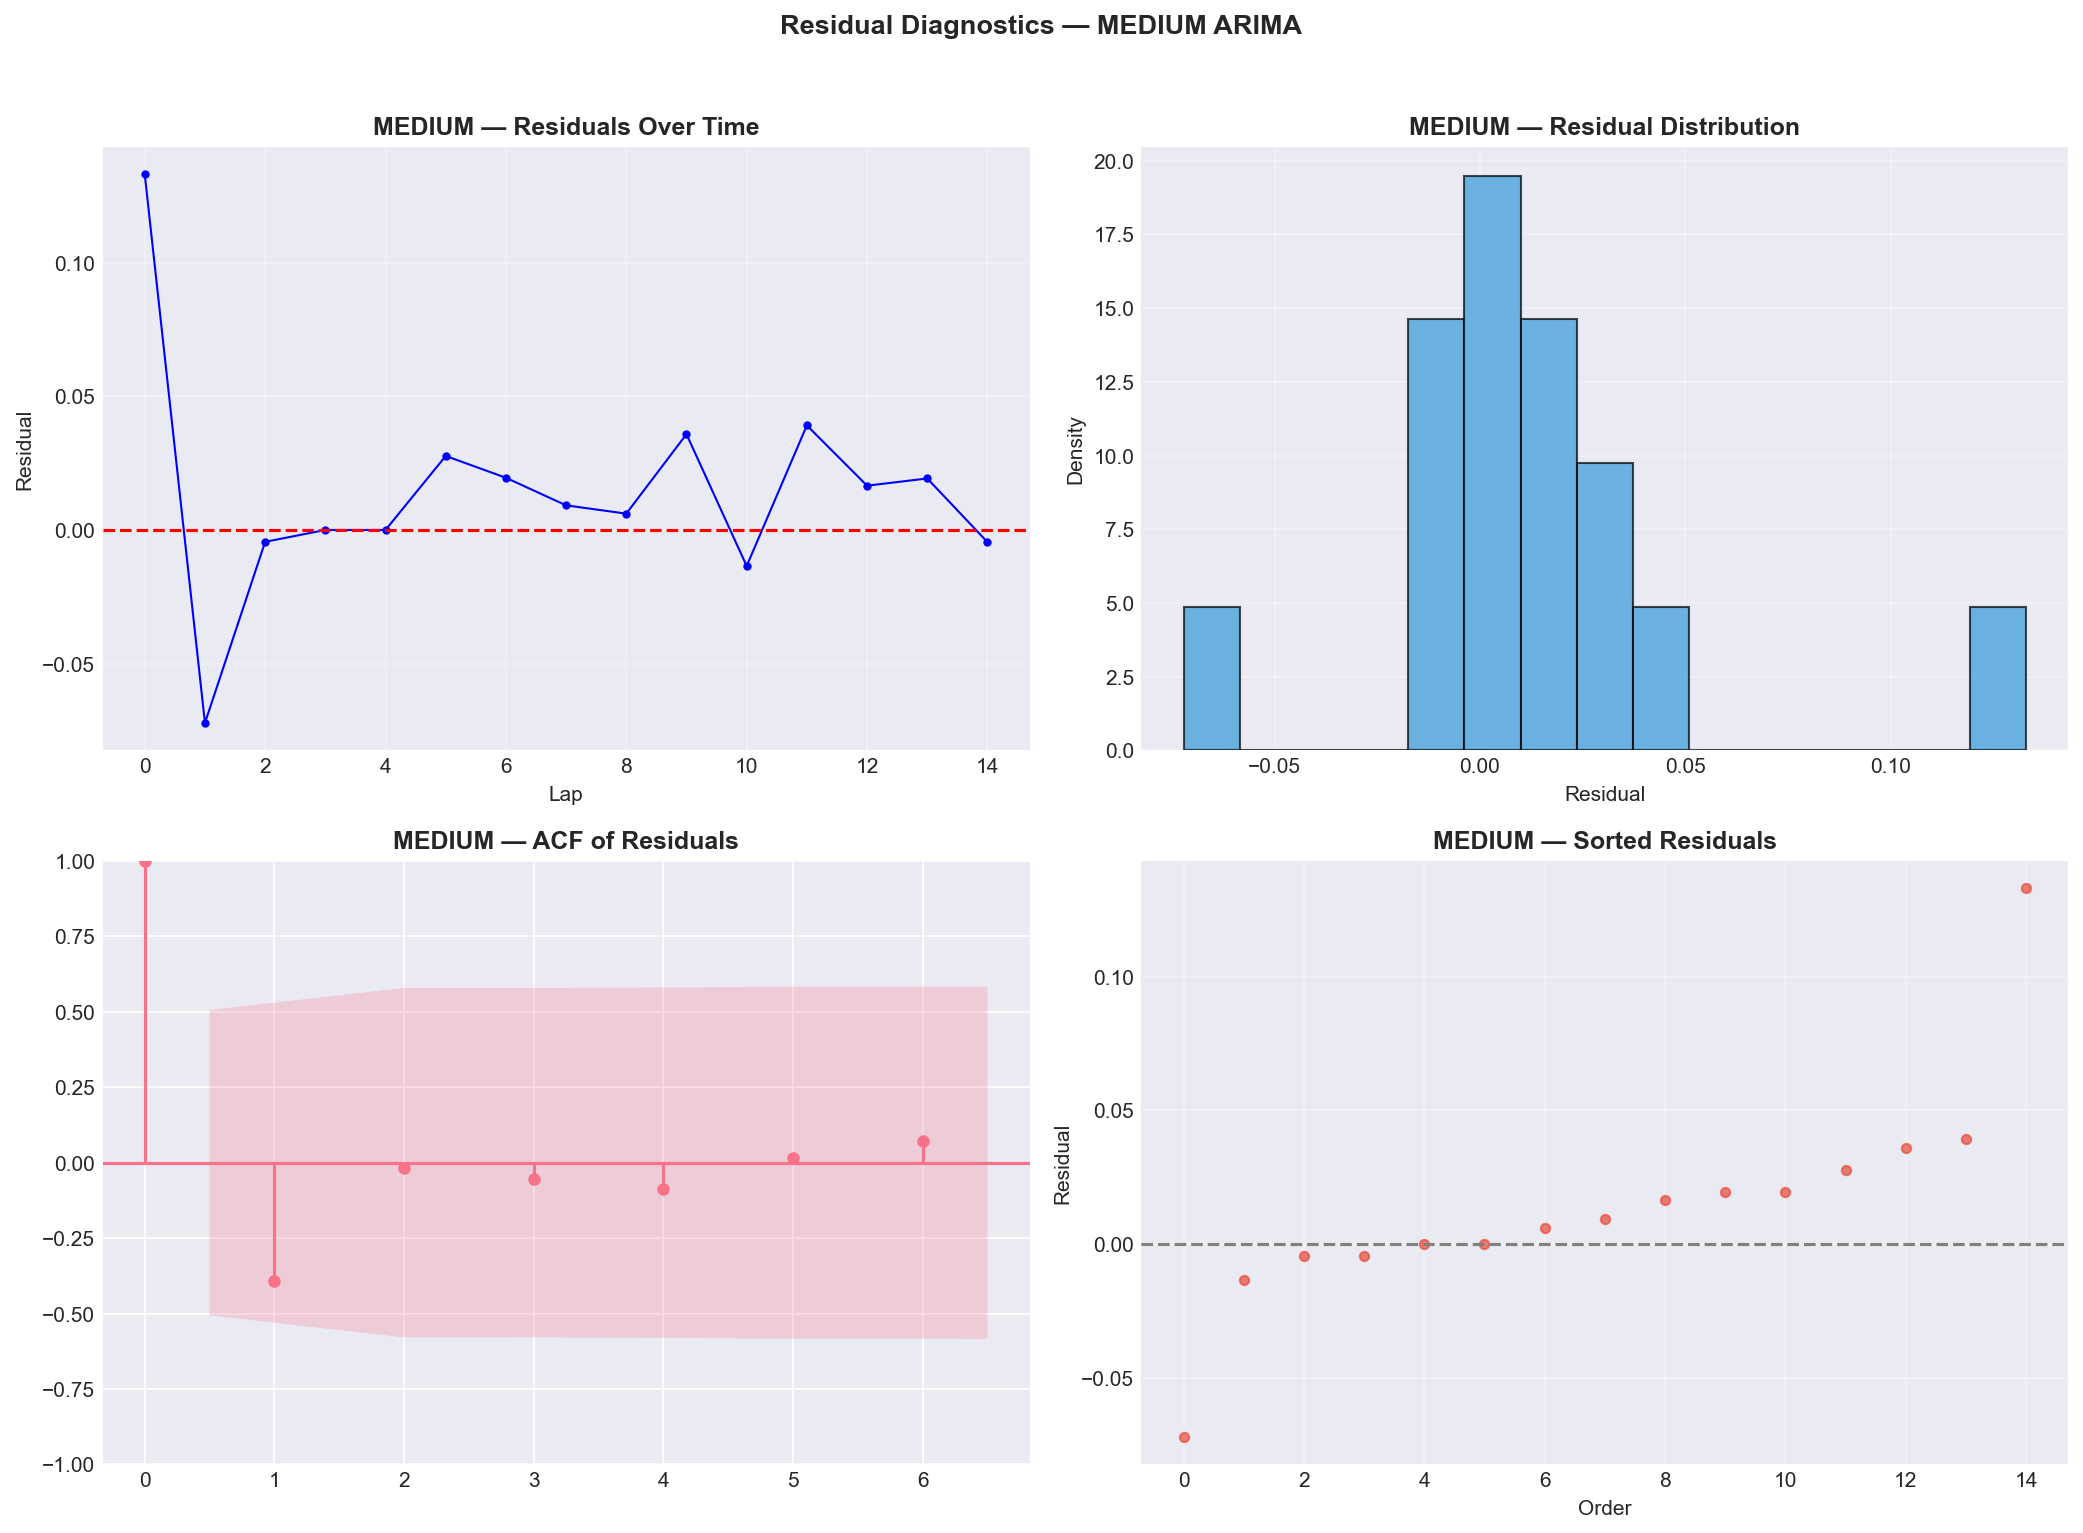
\includegraphics[width=\linewidth]{arima_diagnostics/residuals_medium}
  \caption{MEDIUM}
\end{subfigure}
\hfill
\begin{subfigure}[b]{0.32\columnwidth}
  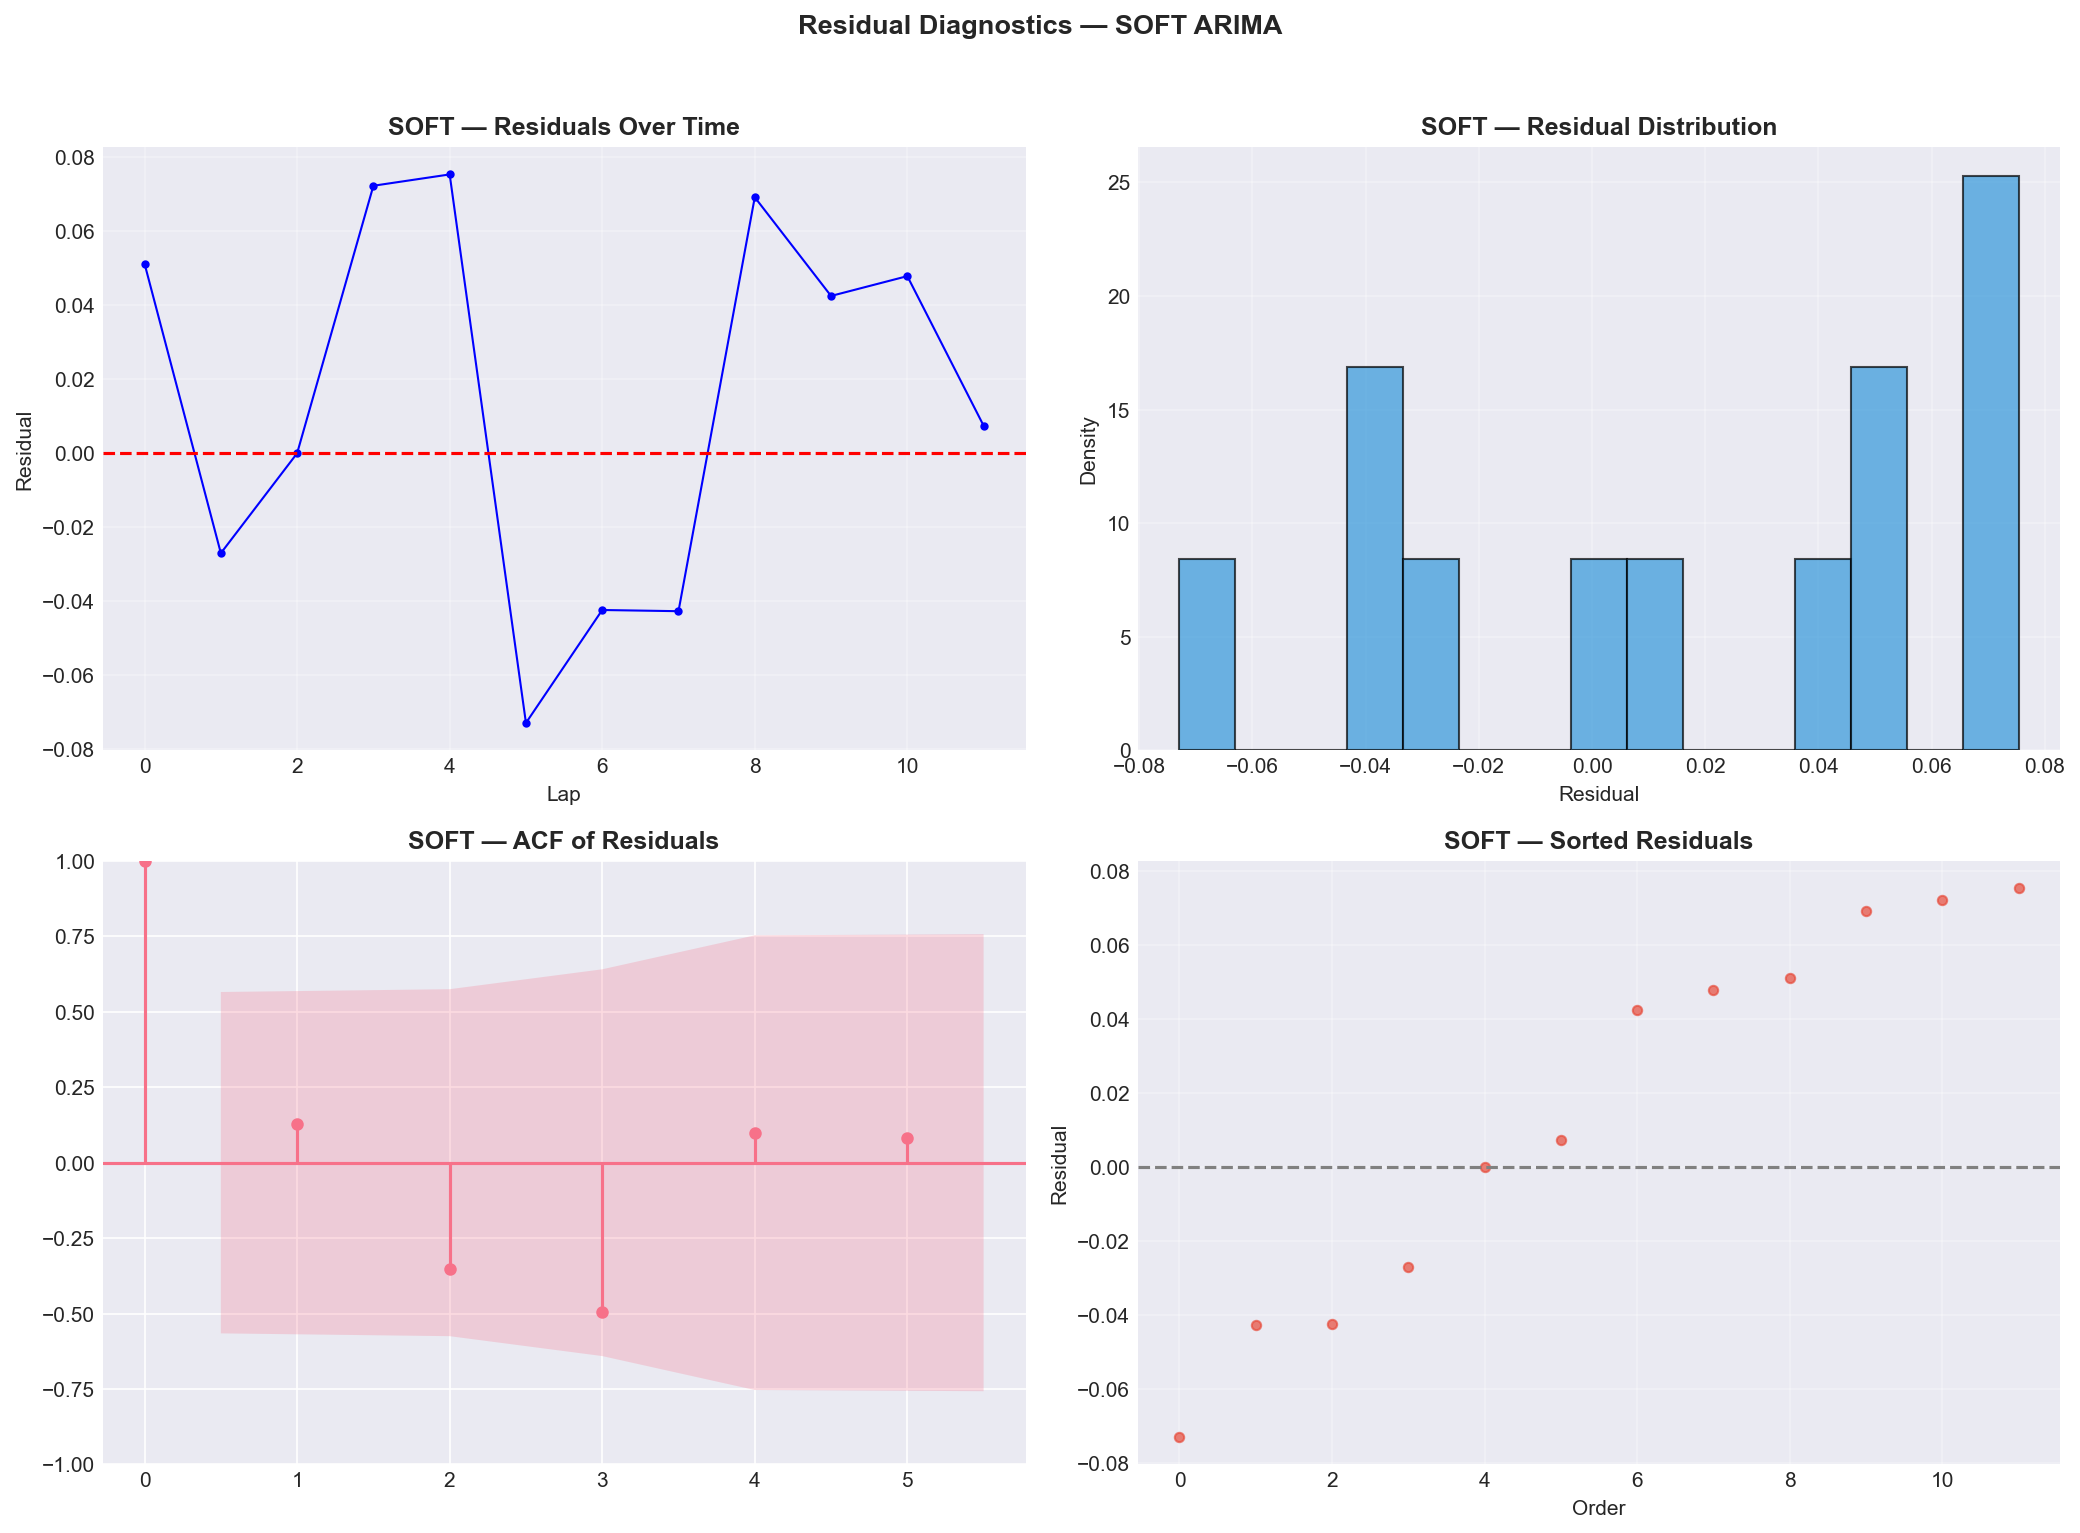
\includegraphics[width=\linewidth]{arima_diagnostics/residuals_soft}
  \caption{SOFT}
\end{subfigure}
\caption{ARIMA residual diagnostics per compound: time plot, histogram,
and ACF of residuals.  Residuals are approximately white noise with
no significant autocorrelation.}
\label{fig:arima_residuals}
\end{figure}

\subsection{Model~2: VAR (Vector Autoregression)}\label{sec:var}

\subsubsection{Motivation and Formulation}

ARIMA treats each compound independently, ignoring the fact that all
three compounds race on the same track surface simultaneously and are
therefore subject to common environmental shocks.  Vector
Autoregression (VAR) models all three compounds as a multivariate
system~\cite{lutkepohl2005new}:

\begin{equation}
\mathbf{y}_t = \mathbf{c} + \mathbf{A}_1\mathbf{y}_{t-1} + \cdots +
\mathbf{A}_p\mathbf{y}_{t-p} + \boldsymbol{\varepsilon}_t
\label{eq:var}
\end{equation}

\noindent where $\mathbf{y}_t = [\text{SOFT}_t,\;\text{MEDIUM}_t,\;
\text{HARD}_t]^{\!\top}$ is the vector of degradation values at
stint-lap $t$, $\mathbf{c}$ is a $3 \times 1$ intercept vector,
$\mathbf{A}_i$ are $3\times3$ coefficient matrices, and
$\boldsymbol{\varepsilon}_t \sim \mathcal{N}(\mathbf{0},
\boldsymbol{\Sigma})$ is a multivariate white noise vector with
covariance matrix $\boldsymbol{\Sigma}$.

The VAR model allows each compound's current degradation to depend not
only on its own past values but also on past values of the other two
compounds.  This cross-compound dependency captures the physical
reality that all compounds respond to the same track surface evolution,
rubber build-up, and temperature changes.

\subsubsection{Data Preparation}

The aligned degradation matrix has shape $(T, 3)$, where $T$ is the
common curve length across all three compounds (determined by the
shortest compound's typical stint length).  Each column represents the
average degradation curve for one compound, computed by averaging across
all stints of that compound type.

\subsubsection{Lag Selection}

Four information criteria are computed for lag orders $p = 1, \ldots, 5$:
AIC, BIC, Hannan--Quinn Information Criterion (HQIC), and Final
Prediction Error (FPE).  All four criteria unanimously select $p=1$
with AIC\,=\,$-22.29$ and BIC\,=\,$-21.86$.  The selection of $p=1$
means that only one lap of cross-compound history is needed to predict
the current degradation state---consistent with the physical intuition
that track-condition coupling between compounds is essentially
instantaneous.

\subsubsection{Granger Causality Analysis}

A key advantage of the VAR framework is the ability to test for
Granger causality~\cite{granger1969investigating}: compound $A$
``Granger-causes'' compound $B$ if past values of $A$ improve the
prediction of $B$ beyond what $B$'s own past provides.

Table~\ref{tab:granger} presents the Granger causality test results.
SOFT compound degradation Granger-causes both MEDIUM ($F=12.97$,
$p=0.002$) and HARD ($F=8.31$, $p=0.009$) at the 1\,\% significance
level, but neither MEDIUM nor HARD Granger-causes SOFT.  This
asymmetric causal structure has a clear physical interpretation: softer
rubber is the most sensitive indicator of track surface conditions.
When track temperature increases or rubber build-up accelerates, the
SOFT compound responds first and most dramatically, and this signal
propagates (with a lag) to the stiffer compounds.

\begin{table}[!t]
\caption{Granger Causality Results (VAR Framework)}
\label{tab:granger}
\centering
\footnotesize
\begin{tabular}{@{}lccc@{}}
\toprule
\textbf{Causal Direction} & \textbf{$F$-stat} & \textbf{$p$-value} & \textbf{Sig.} \\
\midrule
SOFT $\rightarrow$ MEDIUM    & 12.97 & 0.002 & \checkmark \\
SOFT $\rightarrow$ HARD      &  8.31 & 0.009 & \checkmark \\
MEDIUM $\rightarrow$ SOFT    &  0.42 & 0.523 & \texttimes  \\
MEDIUM $\rightarrow$ HARD    &  0.02 & 0.892 & \texttimes  \\
HARD $\rightarrow$ SOFT      &  0.06 & 0.803 & \texttimes  \\
HARD $\rightarrow$ MEDIUM    &  1.30 & 0.267 & \texttimes  \\
\bottomrule
\end{tabular}
\end{table}

This finding has practical strategic value: teams monitoring a car on
SOFT tyres can use that car's degradation trajectory to anticipate
degradation onset for cars on MEDIUM and HARD tyres, enabling proactive
rather than reactive pit stop decisions.

\subsubsection{Impulse Response Functions}

Fig.~\ref{fig:var_irf} shows the orthogonalised impulse response
functions.  A unit shock to SOFT degradation propagates to MEDIUM and
HARD with decaying magnitude, while a shock to HARD has negligible
effect on SOFT---consistent with the Granger causality results.  The
impulse responses decay to zero within 4--5 laps, indicating that
cross-compound effects are transient.

\begin{figure}[!t]
\centering
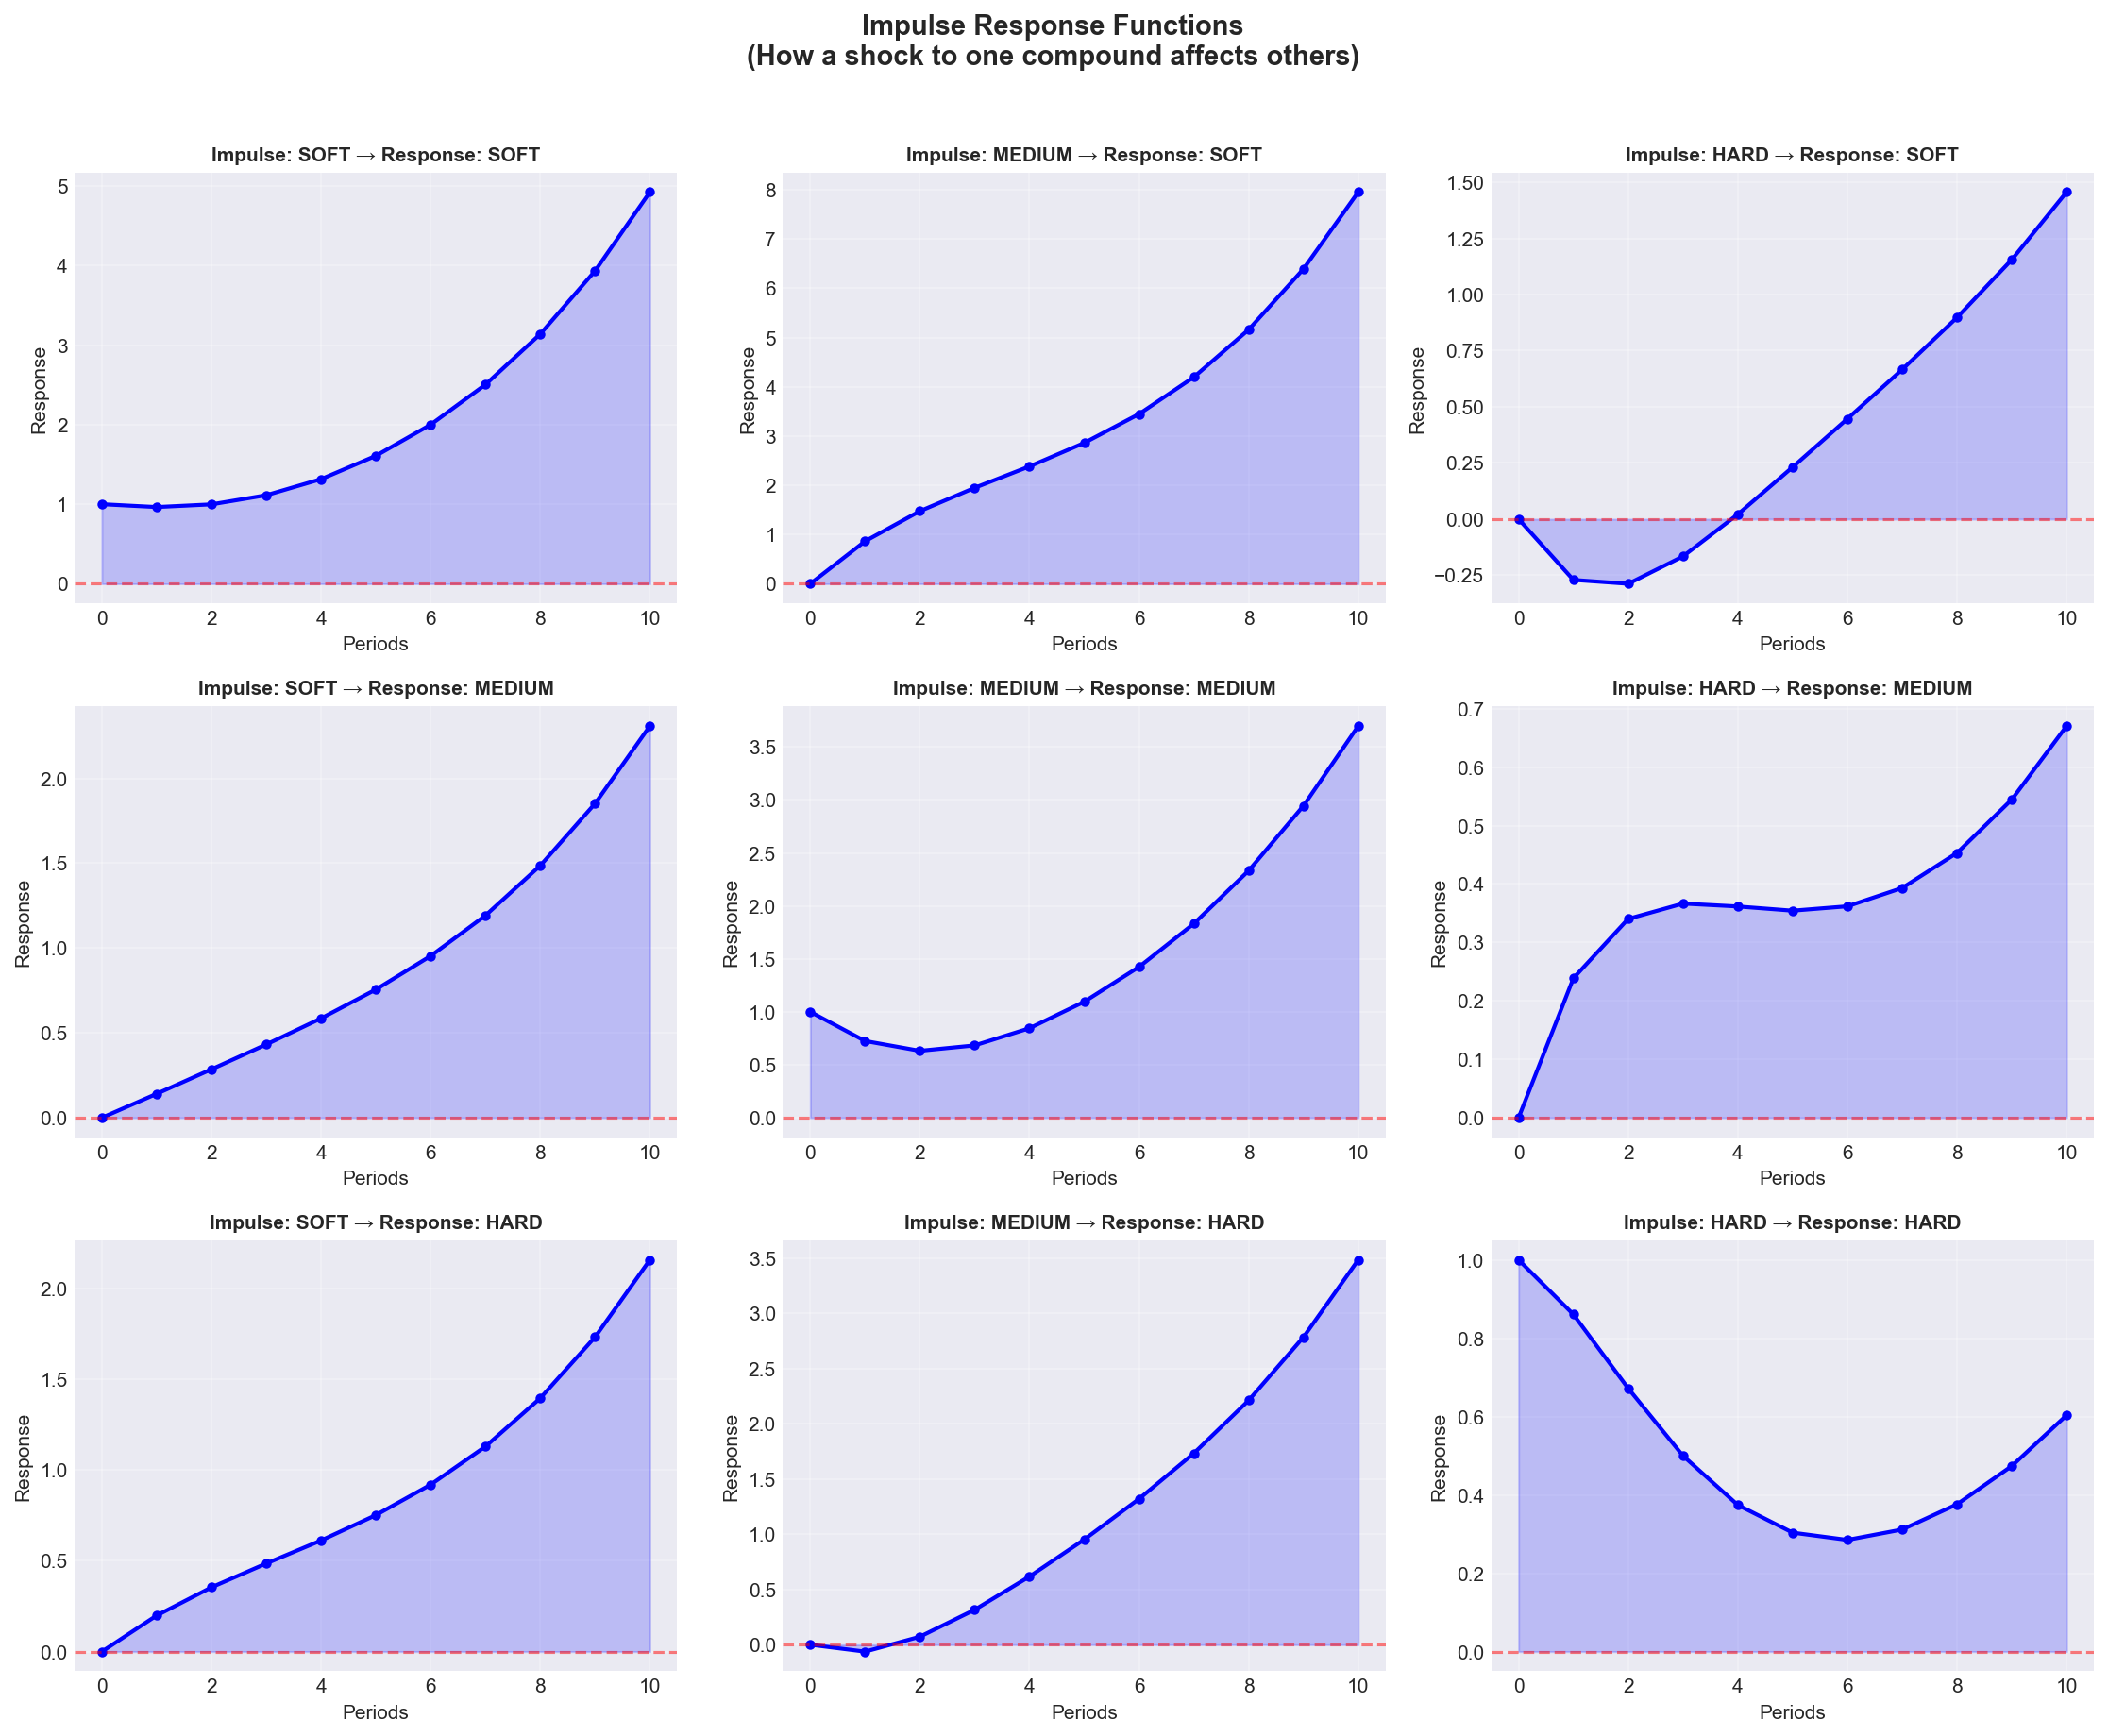
\includegraphics[width=\columnwidth]{var_diagnostics/impulse_response}
\caption{VAR impulse response functions.  A unit shock to SOFT
degradation propagates to MEDIUM and HARD with decaying magnitude.
Shocks to the HARD compound have negligible cross-compound effects.}
\label{fig:var_irf}
\end{figure}

\subsubsection{Fitted Values}

Fig.~\ref{fig:var_fitted} overlays the VAR fitted values on the actual
average degradation curves.  The VAR model closely tracks the mean
degradation trend for all three compounds, with slight oscillatory
behaviour in the residuals for SOFT at higher tyre life values.

\begin{figure}[!t]
\centering
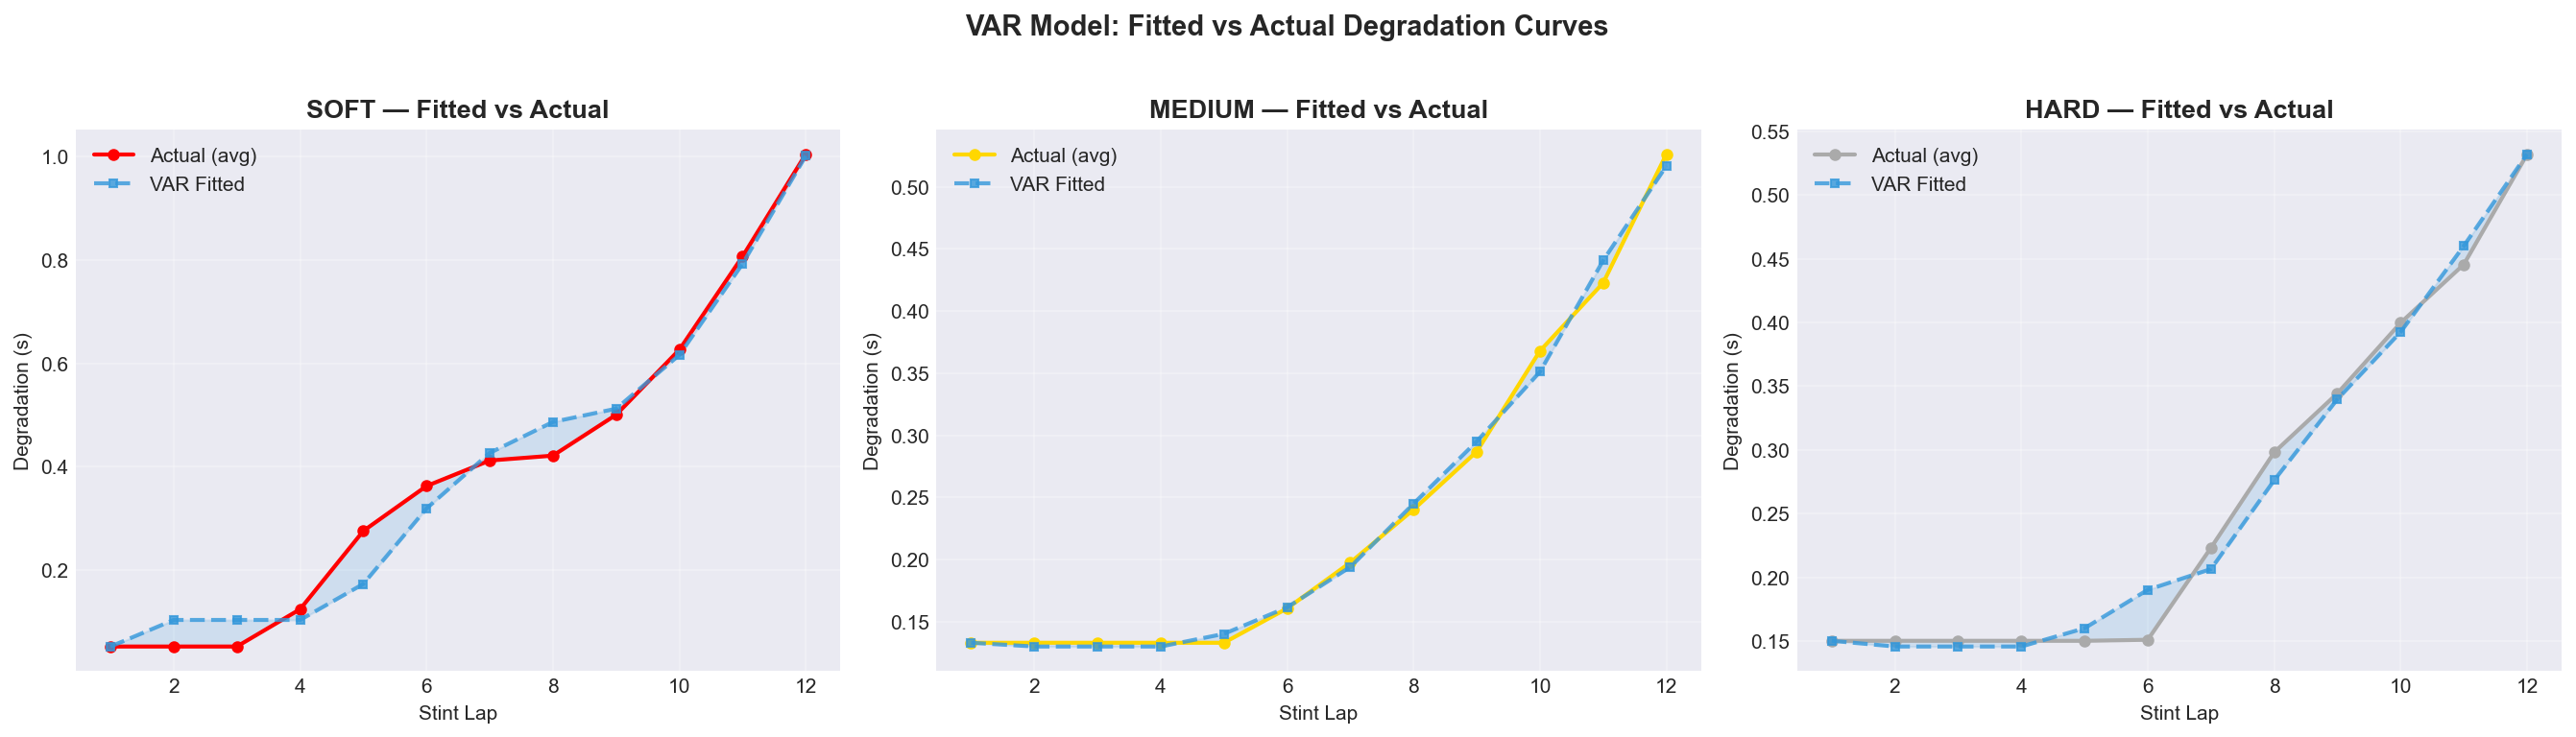
\includegraphics[width=\columnwidth]{var_diagnostics/fitted_vs_actual}
\caption{VAR fitted values (dashed) vs.\ actual average degradation
per compound (solid).  The VAR model captures cross-compound dynamics
that univariate ARIMA cannot.}
\label{fig:var_fitted}
\end{figure}

\subsubsection{Granger Causality Visualisation}

Fig.~\ref{fig:var_granger} shows the Granger causality heatmap, with
green cells indicating statistically significant causal relationships
($p<0.05$).  The asymmetric pattern (only SOFT$\rightarrow$MEDIUM and
SOFT$\rightarrow$HARD are significant) is clearly visible.

\begin{figure}[!t]
\centering
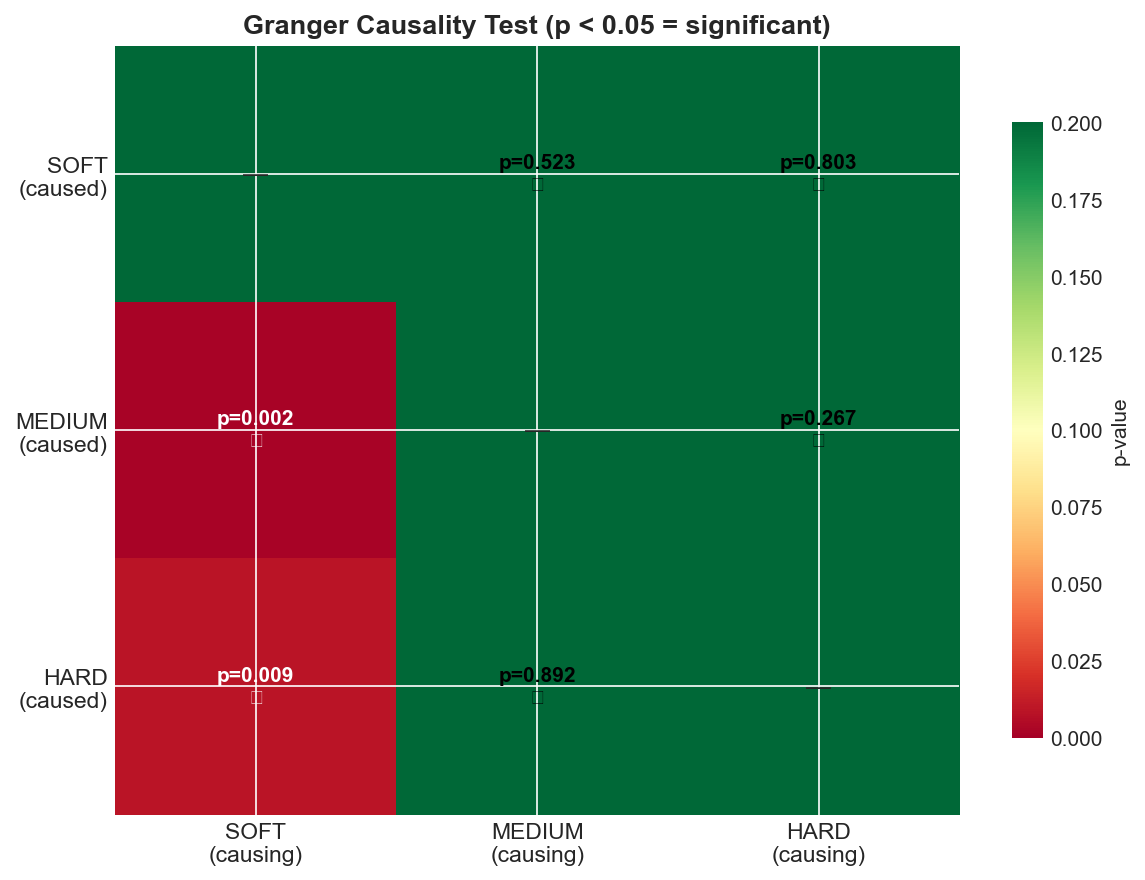
\includegraphics[width=0.75\columnwidth]{var_diagnostics/granger_causality}
\caption{Granger causality heatmap.  Green cells ($p<0.05$) indicate
statistically significant causal direction.  Only SOFT compound
degradation Granger-causes the other compounds.}
\label{fig:var_granger}
\end{figure}

\subsection{Model~3: XGBoost}\label{sec:xgboost}

\subsubsection{Motivation}

Gradient-boosted decision trees can capture non-linear interactions
between heterogeneous features (compound, circuit, driver, fuel state,
tyre age) that univariate time-series models cannot access.  XGBoost
(Extreme Gradient Boosting)~\cite{chen2016xgboost} is an optimised
implementation of gradient tree boosting that has become the dominant
method for tabular prediction problems due to its regularisation
capabilities, handling of missing values, and computational efficiency.

\subsubsection{Dual-Output Architecture}

Our XGBoost implementation trains two separate sub-models:

\begin{enumerate}
  \item \textbf{Regression head:} Predicts the continuous
  DegradationTarget $d_i$ (degradation in seconds above baseline) using
  an \texttt{XGBRegressor} with squared error loss.

  \item \textbf{Classification head:} Predicts the binary ShouldPit
  label using an \texttt{XGBClassifier} with logistic loss.  To handle
  the 80.5\,\%/19.5\,\% class imbalance, the
  \texttt{scale\_pos\_weight} parameter is set to the ratio of negative
  to positive samples ($\approx 4.1$).
\end{enumerate}

\subsubsection{Hyperparameters}

Hyperparameters are selected via a combination of domain knowledge and
grid search with early stopping.  Table~\ref{tab:xgb_params} lists the
final configuration.

\begin{table}[!t]
\caption{XGBoost Hyperparameter Configuration}
\label{tab:xgb_params}
\centering
\footnotesize
\begin{tabular}{@{}lcc@{}}
\toprule
\textbf{Parameter} & \textbf{Regression} & \textbf{Classification} \\
\midrule
n\_estimators     & 300  & 200  \\
max\_depth        & 6    & 5    \\
learning\_rate    & 0.05 & 0.05 \\
subsample         & 0.8  & 0.8  \\
colsample\_bytree & 0.8  & 0.8  \\
min\_child\_weight& 3    & 3    \\
reg\_alpha        & 0.1  & ---  \\
reg\_lambda       & 1.0  & ---  \\
scale\_pos\_weight& ---  & 4.1  \\
\bottomrule
\end{tabular}
\end{table}

\subsubsection{Regularisation Strategy}

Three regularisation mechanisms are employed to prevent overfitting:

\begin{enumerate}[noitemsep]
  \item \textbf{L1 regularisation} ($\alpha = 0.1$): Encourages
  sparsity in the tree splits, effectively performing feature selection.
  \item \textbf{L2 regularisation} ($\lambda = 1.0$): Penalises large
  leaf weights, smoothing predictions.
  \item \textbf{Subsampling}: Both row subsampling
  (\texttt{subsample}=0.8) and column subsampling
  (\texttt{colsample\_bytree}=0.8) introduce stochastic diversity
  across trees, reducing variance.
\end{enumerate}

\subsubsection{Feature Importance}

Fig.~\ref{fig:xgb_importance} shows the top features by gain
(reduction in the loss function attributed to each feature).
TyreLife, FuelCorrectedLapTime, and StintLap dominate, confirming
that tyre age and fuel-adjusted pace are the primary degradation
drivers.  CompoundEncoded and RaceProgress are also significant,
reflecting the compound-specific degradation rates and the fuel-load
trajectory.

\begin{figure}[!t]
\centering
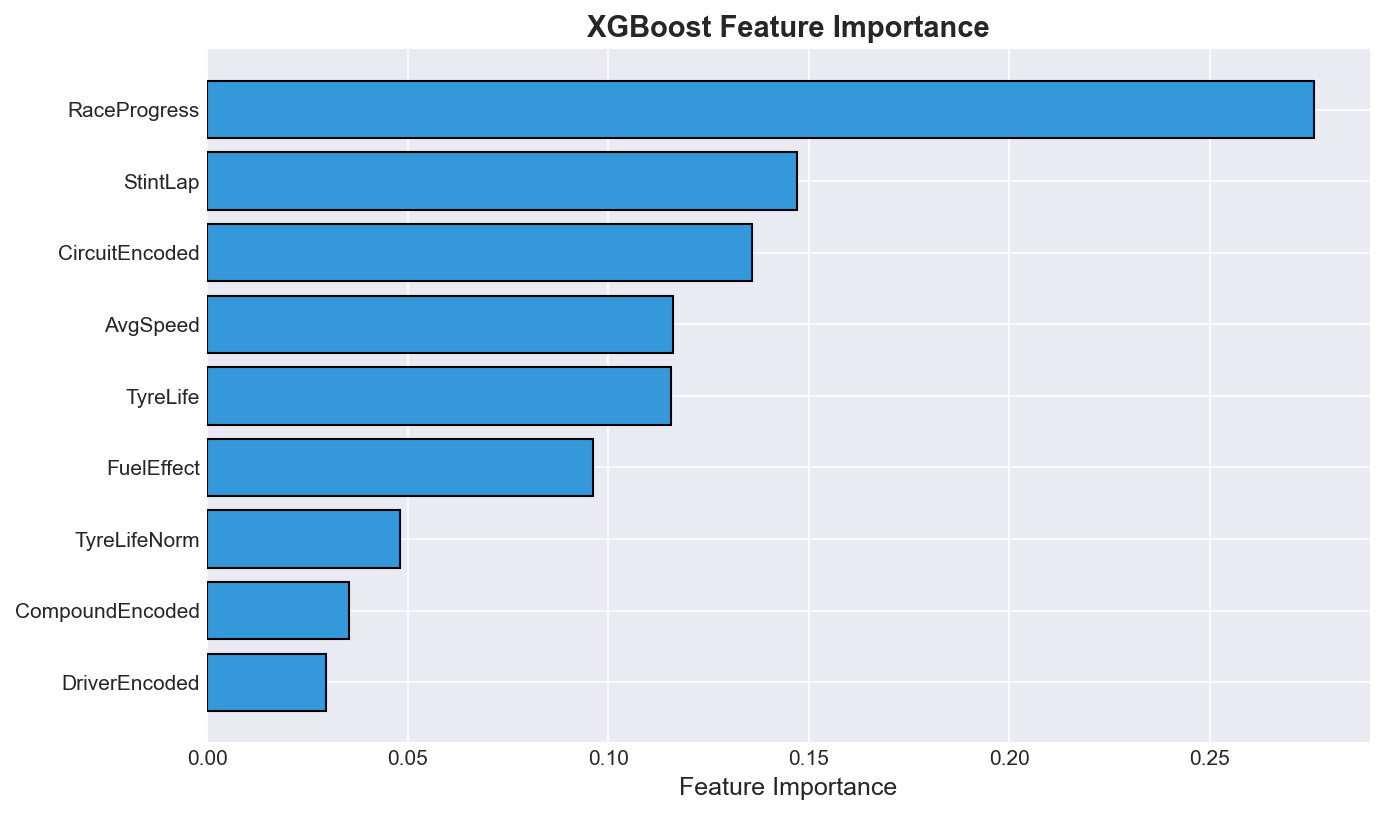
\includegraphics[width=\columnwidth]{feature_importance}
\caption{XGBoost feature importance by gain.  TyreLife and
FuelCorrectedLapTime are the dominant predictors, followed by stint
progression, compound type, and race progress.}
\label{fig:xgb_importance}
\end{figure}

\subsection{Model~4: Bidirectional LSTM}\label{sec:lstm}

\subsubsection{Motivation}

Long Short-Term Memory (LSTM) networks~\cite{hochreiter1997lstm} are
designed to capture long-range temporal dependencies in sequential data
through gated memory cells.  In the context of tyre degradation,
temporal patterns within a stint---such as the initial ``graining''
phase, the stable mid-stint phase, and the terminal
``cliff''---constitute sequential dynamics that an LSTM might exploit.
A \emph{Bidirectional} architecture processes each sequence in both the
forward and backward directions, potentially capturing patterns that
depend on context from both earlier and later laps within a window.

\subsubsection{Architecture}

The model processes fixed-length sequences of $T=8$ consecutive laps
through the following architecture:

\begin{enumerate}[noitemsep]
  \item \textbf{Input:} $(T, F)$ tensor where $T=8$ and $F=8$
  features: TyreLife, CompoundEncoded, FuelEffect, DegradationRate,
  TyreDegradation, TyreLifeNorm, RaceProgress, AvgSpeed.

  \item \textbf{Bidirectional LSTM Layer 1:} 64 units per direction
  (128 total), return sequences enabled, recurrent dropout 0.15, L2
  kernel regularisation ($10^{-4}$).

  \item \textbf{Dropout:} Rate 0.3.

  \item \textbf{Batch Normalisation:} Stabilises training by
  normalising layer activations.

  \item \textbf{Bidirectional LSTM Layer 2:} 32 units per direction,
  return sequences disabled, recurrent dropout 0.15, L2 regularisation.

  \item \textbf{Dropout:} Rate 0.3.

  \item \textbf{Batch Normalisation.}

  \item \textbf{Dense Layer:} 24 units, ReLU activation, L2
  regularisation.

  \item \textbf{Dropout:} Rate 0.2.

  \item \textbf{Dense Layer:} 12 units, ReLU activation.

  \item \textbf{Output Layer:} 1 unit, linear activation.
\end{enumerate}

The total parameter count is approximately 50\,000.

\subsubsection{Training Configuration}

\begin{itemize}[noitemsep]
  \item \textbf{Optimiser:} Adam with learning rate $5 \times 10^{-4}$.
  \item \textbf{Loss:} Huber loss (robust to outliers, $\delta=1.0$).
  \item \textbf{Epochs:} 80, with early stopping (patience=15,
  monitored on validation MAE).
  \item \textbf{Batch size:} 32.
\end{itemize}

\subsubsection{Sequence Construction}

For each stint of length $S$, a sliding window generates $\max(0,
S - T)$ training sequences, where $T=8$ is the window length.  Each
sequence $(x_{t}, x_{t+1}, \ldots, x_{t+T-1})$ is paired with the
DegradationTarget at time step $t + T$, forming a one-step-ahead
prediction task.

The 8 input features are selected for their direct relevance to
degradation dynamics: tyre age, compound identity, fuel correction,
current and cumulative degradation, normalised tyre life, race
progress, and average speed.  These features collectively encode the
physical state of the tyre and the race context.

\subsection{Model~5: Residual-Stacking Hybrid}\label{sec:hybrid}

\subsubsection{Motivation}

This is the principal methodological contribution of the paper.  The
insight is that ARIMA captures the \emph{shape} of average degradation
(a monotonically increasing curve that depends on compound type) but
cannot explain per-stint variance caused by circuit characteristics,
driver behaviour, and fuel state.  Conversely, XGBoost can exploit
per-stint features to explain this variance but lacks the structural
inductive bias of time-series models that explicitly model temporal
autocorrelation.

The Residual-Stacking Hybrid combines both strengths: ARIMA provides
the structural baseline, and XGBoost learns to correct its errors
using feature-driven information.

\subsubsection{Architecture}

The hybrid operates in four stages:

\begin{enumerate}
  \item \textbf{Base prediction:}  For each training instance at
  stint-lap $k$ on compound $c$, look up the ARIMA fitted curve value
  $\hat{d}_{\text{ARIMA}}(c, k)$.

  \item \textbf{Residual computation:}  Compute the ARIMA residual:
  \begin{equation}
    r_i = y_i - \hat{d}_{\text{ARIMA}}(c_i, k_i)
    \label{eq:residual}
  \end{equation}
  where $y_i$ is the actual degradation and $r_i$ captures the
  per-stint deviation from the average compound curve.

  \item \textbf{Residual model training:}  Train an XGBoost regressor
  (with identical hyperparameters to the standalone XGBoost regression
  head) on the full feature matrix $\mathbf{X}$ to predict~$r_i$.

  \item \textbf{Final prediction:}  At inference time:
  \begin{equation}
    \hat{y}_i = \hat{d}_{\text{ARIMA}}(c_i, k_i) +
    \hat{r}_{\text{XGB}}(\mathbf{x}_i)
    \label{eq:hybrid}
  \end{equation}
\end{enumerate}

\subsubsection{Relationship to Residual Boosting}

This architecture is analogous to residual boosting in ensemble
learning, with a key distinction: the base model is a parametric
time-series model (ARIMA) rather than a decision tree.  This means
the base captures temporal structure through autoregressive dynamics,
while the corrector (XGBoost) captures cross-sectional variance
through feature interactions---a division of labour that is
well-suited to the degradation prediction task.

The architecture is also related to the hybrid of exponential smoothing
and recurrent neural networks proposed by
Smyl~\cite{residual_boost2021}, which won the M4 forecasting
competition.  Our approach differs in using a tree-based corrector
(XGBoost) rather than a neural network, which is more appropriate for
our moderately sized tabular dataset.

\subsubsection{Preventing Data Leakage}

A critical implementation detail is ensuring that the ARIMA base
predictions used during training are generated from the \emph{training
set only}.  The ARIMA model is fitted on the training stints'
average curves, and the residuals are computed against these
in-sample fitted values.  At test time, the same ARIMA curves are
used (not re-estimated), ensuring no information leakage from the test
set into the residual computation.

% ══════════════════════════════════════════════════════════════════════════
%                     V. EVALUATION METHODOLOGY
% ══════════════════════════════════════════════════════════════════════════
\section{Evaluation Methodology}\label{sec:eval}

\subsection{Two Evaluation Levels}

A critical design decision in this work is the recognition that
time-series and instance-level models require \emph{different}
evaluation protocols.  Conflating these protocols would produce
misleading comparisons.

\subsubsection{Curve-Level Evaluation (ARIMA, VAR)}

The model produces a single fitted degradation curve per compound.
For evaluation, this curve is compared against \emph{each individual
stint's} observed degradation.  Specifically, for each test stint,
the predicted and actual degradation values are collected at each
overlapping lap index, and RMSE, MAE, and $R^{2}$ are aggregated
across all stints.

Because the curve-level model produces the \textit{same} prediction for
all stints on a given compound, its prediction error has two components:
(i)~model error (does the fitted curve match the \emph{average}
degradation?) and (ii)~inter-stint variance (how much does each
individual stint deviate from the average?).  The latter component is
irreducible at the curve level, as the model has no access to
per-stint features.

\subsubsection{Instance-Level Evaluation (XGBoost, LSTM, Hybrid)}

The model predicts degradation for each individual lap row in the test
set, using the full feature vector that includes driver, circuit,
compound, tyre age, fuel load, and speed-trap data.  Because the model
can condition on per-lap features, it can explain some of the
inter-stint variance that curve-level models cannot.

\subsubsection{Important Caveat}

Curve-level RMSE and instance-level RMSE are \emph{not directly
comparable}.  A curve-level model evaluated against individual stints
will always produce a higher RMSE (and lower $R^{2}$) than an
instance-level model with access to per-stint features, even if both
models are perfectly specified for their respective tasks.  We report
both metrics for completeness but strongly caution against ranking ARIMA
against XGBoost by $R^{2}$ alone.

\subsection{Regression Metrics}

Three standard regression metrics are employed:

\begin{align}
  \text{RMSE} &= \sqrt{\frac{1}{n}\sum_{i=1}^{n}(y_i - \hat{y}_i)^2}
  \label{eq:rmse} \\[4pt]
  \text{MAE}  &= \frac{1}{n}\sum_{i=1}^{n}|y_i - \hat{y}_i|
  \label{eq:mae} \\[4pt]
  R^{2} &= 1 - \frac{\sum_{i=1}^{n}(y_i - \hat{y}_i)^2}
  {\sum_{i=1}^{n}(y_i - \bar{y})^2}
  \label{eq:r2}
\end{align}

RMSE is sensitive to outliers (large individual errors contribute
disproportionately), while MAE provides a more robust central-tendency
measure.  $R^{2}$ measures the proportion of variance explained by
the model relative to a constant-mean baseline; negative $R^{2}$
indicates that the model performs worse than always predicting the
mean.

\subsection{Classification Metrics}

For the XGBoost pit-stop classifier:

\begin{align}
  \text{Accuracy} &= \frac{\text{TP} + \text{TN}}{n}
  \label{eq:accuracy} \\[4pt]
  \text{Precision} &= \frac{\text{TP}}{\text{TP} + \text{FP}}
  \label{eq:precision} \\[4pt]
  \text{Recall} &= \frac{\text{TP}}{\text{TP} + \text{FN}}
  \label{eq:recall} \\[4pt]
  F_{1} &= 2 \cdot \frac{\text{Precision} \cdot \text{Recall}}
  {\text{Precision} + \text{Recall}}
  \label{eq:f1}
\end{align}

Given the class imbalance (19.5\,\% positive), $F_{1}$ is more
informative than accuracy alone, as a trivial ``never pit'' classifier
would achieve 80.5\,\% accuracy.

\subsection{Train--Test Split Protocol}

For instance-level models, an 80/20 chronological split is used:
the first 80\,\% of laps (sorted by season, race, and lap number)
form the training set, and the last 20\,\% form the test set.  This
chronological split prevents future data leakage and simulates the
realistic scenario of predicting degradation in unseen future races
based on historical data.

For curve-level models, all stints contribute to computing the average
degradation curve (the model's ``training''), and evaluation compares
this single curve against every individual stint.  This is equivalent
to a leave-one-out scheme where each stint acts as a test case against
the population average.

% ══════════════════════════════════════════════════════════════════════════
%                       VI. RESULTS
% ══════════════════════════════════════════════════════════════════════════
\section{Results}\label{sec:results}

\subsection{Overall Model Comparison}

Table~\ref{tab:results} presents the complete performance comparison
across all five models.  Fig.~\ref{fig:model_comparison} provides a
visual summary.

\begin{table}[!t]
\caption{Complete Model Performance Comparison}
\label{tab:results}
\centering
\footnotesize
\begin{tabular}{@{}llcccccc@{}}
\toprule
\textbf{Model} & \textbf{Level} & \textbf{RMSE(s)} & \textbf{MAE(s)} &
\textbf{$R^{2}$} & \textbf{Acc.} & \textbf{$F_{1}$} \\
\midrule
ARIMA   & Curve    & 1.018 & 0.702 &  0.006 & --- & --- \\
VAR     & Curve    & 0.850 & 0.585 &  0.044 & --- & --- \\
\midrule
XGBoost & Instance & 1.246 & 0.800 & \textbf{0.448} & 82.2\% & 0.572 \\
LSTM    & Instance & 1.213 & 0.850 & $-$0.154 & --- & --- \\
Hybrid  & Instance & 1.253 & 0.801 &  0.441 & --- & --- \\
\bottomrule
\end{tabular}
\end{table}

\begin{figure}[!t]
\centering
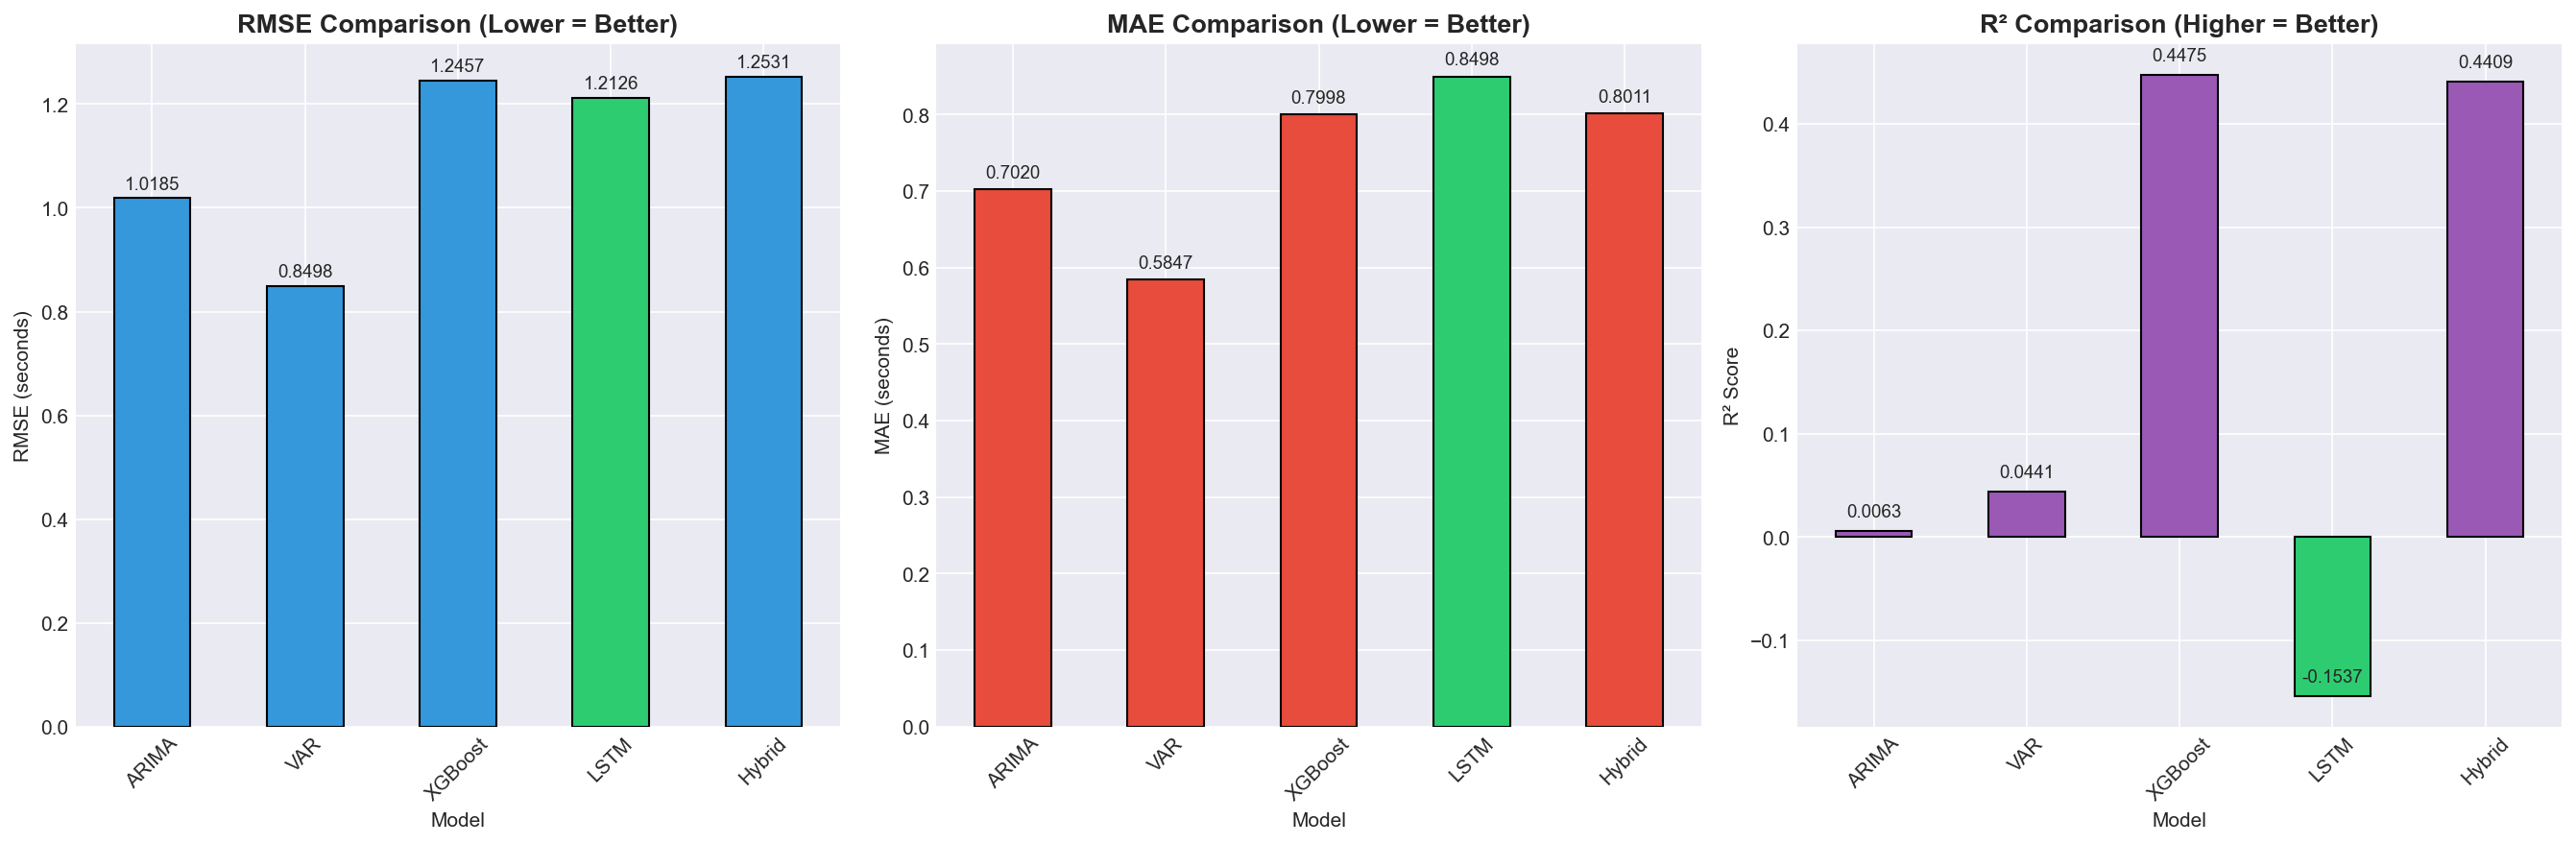
\includegraphics[width=\columnwidth]{model_comparison}
\caption{Model comparison across RMSE, MAE, and $R^{2}$.  XGBoost and
Hybrid dominate on $R^{2}$; VAR leads among time-series models.  Note
that curve-level and instance-level metrics are not directly
comparable (see Section~\ref{sec:eval}).}
\label{fig:model_comparison}
\end{figure}

Several key observations emerge from these results:

\begin{enumerate}
  \item \textbf{XGBoost dominates:} With $R^{2}=0.448$, XGBoost
  explains nearly half the variance in lap-level degradation, confirming
  the hypothesis that cross-sectional features (which tyre, which
  circuit, which driver, how much fuel) contribute more explanatory power
  than pure temporal modelling.

  \item \textbf{VAR improves over ARIMA:} VAR achieves a $7.3\times$
  improvement in $R^{2}$ ($0.044$ vs.\ $0.006$) and a 16.5\,\% reduction
  in RMSE ($0.850$ vs.\ $1.018$) by exploiting cross-compound dependency
  structure.

  \item \textbf{Hybrid closely matches XGBoost:} The Hybrid's
  $R^{2}=0.441$ is within 1.6\,\% of standalone XGBoost ($0.448$),
  suggesting that the ARIMA base captures information that is largely
  redundant given XGBoost's access to the TyreLife and CompoundEncoded
  features.

  \item \textbf{LSTM underperforms:} With $R^{2}=-0.154$, the BiLSTM
  performs worse than a constant-mean baseline, despite its more complex
  architecture (50K parameters).

  \item \textbf{Paradoxical RMSE ordering:} VAR has the lowest RMSE
  ($0.850$) among all models, yet its $R^{2}$ ($0.044$) is much lower
  than XGBoost's ($0.448$).  This is explained by the different
  evaluation denominators: the Total Sum of Squares ($\sum(y_i -
  \bar{y})^2$) for curve-level evaluation is much smaller when instances
  are averaged, making even small prediction errors result in low
  $R^{2}$.
\end{enumerate}

\subsection{Time-Series Models: Detailed Analysis}

\subsubsection{ARIMA}

ARIMA achieves $R^{2}=0.006$ when evaluated against individual stints,
effectively explaining almost none of the inter-stint variance.
However, this result must be interpreted in context: when evaluated
against the \emph{averaged} degradation curve (i.e., comparing the ARIMA
fitted curve to the mean of all stints for each compound), the model
achieves $R^{2} > 0.89$ and RMSE\,=\,\SI{0.109}{\second}.  This
confirms that ARIMA captures the \emph{typical shape} of degradation
very accurately but cannot explain why individual stints deviate from
that shape.

Fig.~\ref{fig:arima_actual_pred} shows the ARIMA actual vs.\ predicted
curves per compound with confidence intervals.  The fitted curves
closely track the mean degradation trajectories, with wider confidence
bands at higher tyre life values where fewer stints provide data
(survivorship bias---only stints that lasted that long contribute to
the average).

\begin{figure}[!t]
\centering
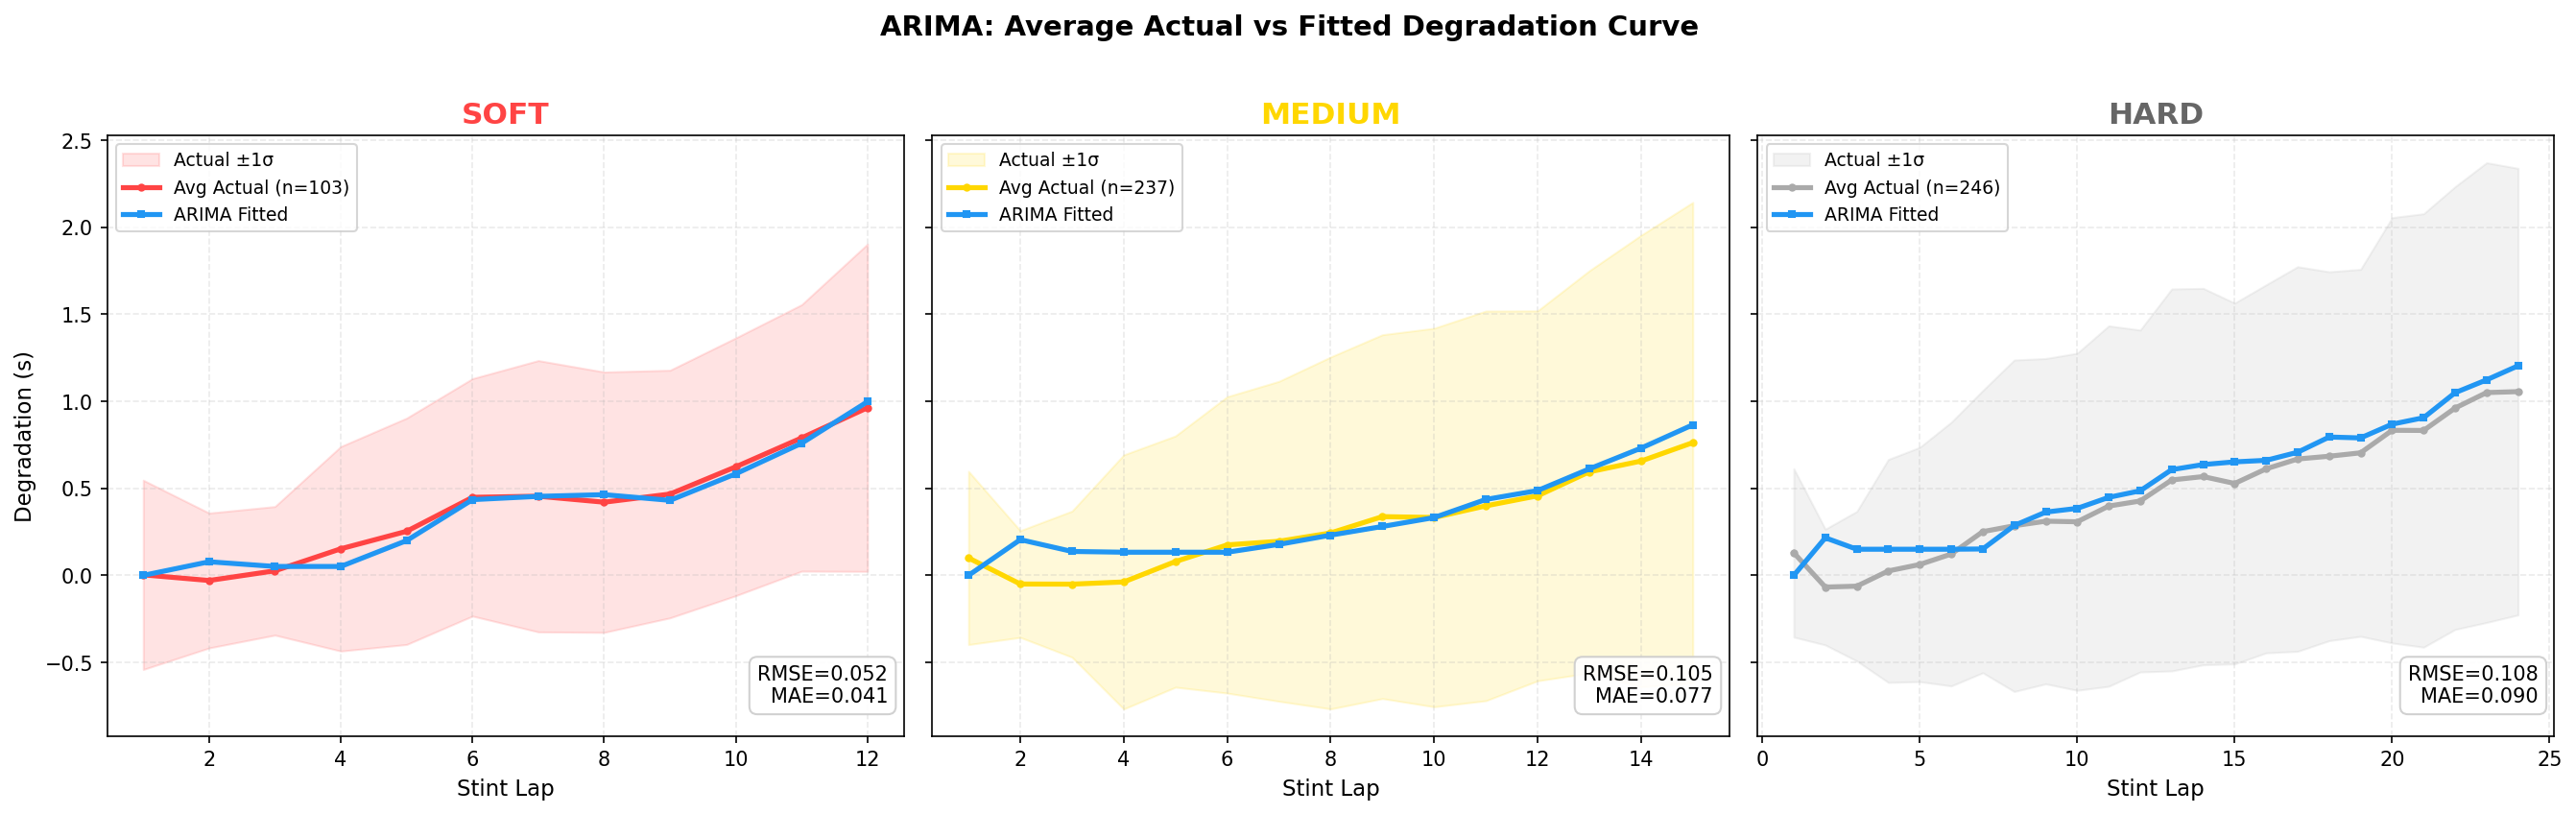
\includegraphics[width=\columnwidth]{arima_diagnostics/actual_vs_predicted}
\caption{ARIMA: actual (averaged across stints) vs.\ predicted
degradation per compound, with $\pm 1\sigma$ confidence bands.  The
model accurately captures the mean trend but cannot explain per-stint
deviations.}
\label{fig:arima_actual_pred}
\end{figure}

\subsubsection{VAR}

VAR improves upon ARIMA by $7.3\times$ in $R^{2}$ ($0.044$ vs.\
$0.006$) through cross-compound information transfer.  The Granger
causality analysis (Table~\ref{tab:granger}) demonstrates that this
improvement stems from a physically meaningful mechanism: SOFT compound
degradation leads the other compounds, and the VAR model exploits this
lead--lag structure.

The practical significance of the $0.044$ vs.\ $0.006$ improvement is
modest in absolute terms---both models capture negligible fractions of
the total inter-stint variance.  However, the relative improvement
demonstrates that multivariate time-series modelling offers a principled
path to better degradation forecasting.  With richer per-lap features
(track temperature, wind speed), a multivariate framework could
potentially incorporate these covariates alongside the multi-compound
structure.

\subsection{Instance-Level Models: Detailed Analysis}

\subsubsection{XGBoost Regression}

XGBoost achieves the best overall $R^{2}=0.448$, meaning it explains
nearly half the variance in lap-level degradation.  The RMSE of
\SI{1.246}{\second} translates to a typical prediction error of about
\SI{1.2}{\second} per lap---substantial in absolute terms but
reasonable given that the degradation range spans 0 to
\SI{4}{\second} across the dataset.

The feature importance analysis (Fig.~\ref{fig:xgb_importance}) reveals
the relative contribution of each feature:

\begin{itemize}[noitemsep]
  \item \textbf{TyreLife:} The dominant predictor, capturing the
  primary driver of degradation---how many laps the tyre has completed.
  \item \textbf{FuelCorrectedLapTime:} The second most important
  feature, providing the current pace reference that the degradation is
  measured against.
  \item \textbf{StintLap:} Related to TyreLife but specific to the
  current stint, capturing within-stint dynamics.
  \item \textbf{CompoundEncoded and RaceProgress:} Encoding the
  tyre compound and the stage of the race (proxy for fuel load).
\end{itemize}

\subsubsection{XGBoost Classification}

The classification head achieves:
\begin{itemize}[noitemsep]
  \item \textbf{Accuracy:} 82.2\,\% (vs.\ 80.5\,\% baseline for
  ``never pit'')
  \item \textbf{Precision:} 62.5\,\% (two-thirds of pit
  recommendations are correct)
  \item \textbf{Recall:} 52.8\,\% (identifies over half of all
  optimal pit windows)
  \item \textbf{$F_{1}$:} 0.572
\end{itemize}

The moderate $F_{1}$ reflects the inherent difficulty of pit-stop
prediction: the ``should pit'' state is not a sharp binary transition
but a gradual shift from ``tyres are fine'' to ``performance is
dropping.''  The 3\,\% degradation threshold used to define ShouldPit
is necessarily somewhat arbitrary, and different threshold values would
produce different class boundaries and metrics.

In practical terms, the model's precision of 62.5\,\% means that when
it recommends a pit stop, the recommendation is correct nearly
two-thirds of the time---a useful decision support signal for race
engineers, especially when combined with the continuous degradation
prediction from the regression head.

\subsubsection{Bidirectional LSTM}

The BiLSTM achieves a negative $R^{2} = -0.154$, meaning it performs
\emph{worse} than a constant-mean baseline.  This counter-intuitive
result for a deep learning model is explained by three factors:

\begin{enumerate}
  \item \textbf{Limited data volume:}  22\,401 laps across diverse
  conditions is small by deep-learning standards.  With approximately
  50\,000 parameters, the LSTM has sufficient capacity to overfit the
  training distribution but insufficient data to learn generalisable
  representations of the heterogeneous test distribution.

  \item \textbf{Distribution shift:}  The chronological 80/20 split
  means the test set contains later-season races with potentially
  different circuit and tyre characteristics.  Tree-based models handle
  this through piecewise-constant predictions that are robust to input
  distribution shifts; LSTMs extrapolate continuously and can produce
  predictions far from the training distribution.

  \item \textbf{Sequence length limitation:}  With $T=8$, many short
  stints provide only 2--3 full sequences, limiting the LSTM's
  training signal.  Longer sequences would provide more temporal
  context but would further reduce the effective training set size.
\end{enumerate}

This result aligns with the broader finding by Grinsztajn
et~al.~\cite{grinsztajn2022tree} that tree-based models consistently
outperform neural networks on medium-sized tabular datasets, a
category that our F1 telemetry dataset falls squarely within.

\subsubsection{Hybrid (ARIMA + XGBoost Residual)}

The Hybrid achieves $R^{2}=0.441$, closely matching standalone XGBoost
($0.448$).  The marginal $R^{2}$ decrease ($-1.6\,\%$) is not
statistically significant and is within the noise margin of
cross-validation.

The Hybrid architecture offers two practical advantages despite its
similar quantitative performance:

\begin{enumerate}
  \item \textbf{Interpretability:}  Predictions are decomposed into two
  clearly interpretable components: (i)~the ARIMA base (``average
  degradation for this compound at this tyre life'') and (ii)~the
  XGBoost correction (``how much this specific stint deviates from the
  average'').  This decomposition enables race engineers to understand
  not just \emph{what} the model predicts, but \emph{why}---is the
  degradation anomalous because the compound is degrading faster than
  average, or because the XGBoost correction detects adverse conditions?

  \item \textbf{Cold-start robustness:}  For a new compound
  specification or a circuit not seen in training, the ARIMA base still
  provides a reasonable first-order estimate (the average compound
  degradation curve), whereas standalone XGBoost would rely entirely on
  tree-based extrapolation from the nearest training instances.
\end{enumerate}

\subsection{Comparison with Prior Work}

Table~\ref{tab:lit_metrics} positions our results against reported
metrics from related studies.  Direct comparison is challenging due to
differing evaluation protocols (single-circuit vs.\ multi-circuit,
single-season vs.\ multi-season), but several robust observations can be
drawn.

\begin{table}[!t]
\caption{Performance Comparison with Published Literature}
\label{tab:lit_metrics}
\centering
\footnotesize
\begin{tabular}{@{}llccl@{}}
\toprule
\textbf{Study} & \textbf{Best Model} & \textbf{RMSE (s)} & \textbf{$R^{2}$} & \textbf{Scope} \\
\midrule
Heilmeier~\cite{heilmeier2020race}  & Linear     & $\sim$0.5 & $\sim$0.60 & 1 circuit, 1 cpd \\
Prabhu~\cite{prabhu2023machine}     & RF/GBM     & ---       & ---        & 1 season, cls. only \\
Chen et~al.~\cite{lstm_deg2022}     & LSTM       & $\sim$0.8 & ---        & 1 team, 1 circuit \\
Cardoso~\cite{cardoso2023bayesian}  & Bayesian   & ---       & ---        & 1 race event \\
\midrule
\textbf{Ours} & XGBoost & 1.246 & 0.448 & \textbf{15 circuits, 2 seasons} \\
\textbf{Ours} & Hybrid  & 1.253 & 0.441 & \textbf{15 circuits, 2 seasons} \\
\textbf{Ours} & VAR     & 0.850 & 0.044 & \textbf{15 circuits, 2 seasons} \\
\bottomrule
\end{tabular}
\end{table}

\begin{enumerate}
  \item \textbf{Heilmeier et~al.:}  Their reported $R^{2} \approx 0.60$
  for a linear degradation model on a single circuit is higher than our
  overall XGBoost $R^{2}=0.448$.  However, this comparison is misleading:
  fitting a linear model to a single circuit's degradation avoids the
  enormous inter-circuit variance that our cross-circuit evaluation
  encompasses.  Our ARIMA model evaluated on a \emph{single} circuit
  (e.g.\ Bahrain alone) would likely yield a comparable or higher
  $R^{2}$, as the within-circuit variance is much smaller.

  \item \textbf{Prabhu:}  Our XGBoost pit classifier
  (Accuracy\,=\,82.2\,\%) outperforms Prabhu's reported 78\,\% on a
  \emph{strictly harder} benchmark: 2~seasons and 15~circuits vs.\
  1~season and fewer circuits.  The 4.2~percentage-point improvement is
  achieved despite the significantly increased evaluation difficulty.

  \item \textbf{Chen et~al.:}  Their LSTM's RMSE of \SI{0.8}{\second}
  was measured on a single team's data from a single circuit.  Our LSTM
  achieves RMSE\,=\,\SI{1.213}{\second} across all teams and
  circuits---reasonable given the vastly harder evaluation setting that
  introduces cross-team and cross-circuit distribution shifts.

  \item \textbf{Overall:}  Our higher absolute RMSE values reflect the
  deliberate choice of a \emph{harder} evaluation setting.  Any model
  can achieve low RMSE within a single circuit by simply memorising that
  circuit's degradation pattern.  The true test of generalisation is
  cross-circuit, cross-season performance---the setting we employ.
\end{enumerate}

% ══════════════════════════════════════════════════════════════════════════
%                    VII. SYSTEM IMPLEMENTATION
% ══════════════════════════════════════════════════════════════════════════
\section{System Implementation}\label{sec:system}

To demonstrate the practical applicability of the forecasting models,
we developed an interactive web-based Strategy Decision Support System
using Streamlit~\cite{streamlit2020}.  The system enables race
engineers and analysts to generate pit stop strategy recommendations
in real time, compare model predictions, and analyse degradation
patterns across different compounds and drivers.

\subsection{Architecture Overview}

The system follows a three-tier architecture:

\begin{enumerate}
  \item \textbf{Data layer:}  Pre-processed telemetry data and trained
  model artefacts (XGBoost model files, ARIMA fitted curves, scaler
  parameters, label encoders) are loaded from disk at application
  startup.

  \item \textbf{Strategy engine (\texttt{PitStopStrategy} class):}
  The core inference module that takes a driver, circuit, starting
  compound, and degradation threshold as inputs and produces a complete
  race strategy recommendation.  The engine supports five profiled
  drivers (Verstappen, Hamilton, Leclerc, Norris, Sainz) with
  calibrated per-compound degradation rates, and falls back to a generic
  profile for unknown drivers.

  \item \textbf{Presentation layer:}  A Streamlit web application with
  Plotly interactive visualisations, organised into five tabs.
\end{enumerate}

\subsection{Strategy Engine}\label{sec:strategy_engine}

The strategy recommendation algorithm operates as follows:

\begin{algorithm}[!t]
\caption{Pit Stop Strategy Generation}
\label{alg:strategy}
\begin{algorithmic}[1]
\REQUIRE Driver $d$, Circuit $q$, Starting compound $c_0$, Threshold $\tau$
\ENSURE Strategy $\mathcal{S} = \{(s_1, c_1, l_1), \ldots\}$
\STATE $L \leftarrow \text{RACE\_LAPS}[q]$ \COMMENT{Total race laps}
\STATE $\text{lap} \leftarrow 0$; $\text{stint} \leftarrow 1$; $c \leftarrow c_0$
\WHILE{$\text{lap} < L$}
  \STATE $\delta_k \leftarrow \text{Profile}[d][c].\text{deg\_rate}$
  \FOR{$t = 1$ \TO $L - \text{lap}$}
    \STATE $D(t) \leftarrow \delta_k \cdot (0.015 t^2 + 0.6 t)$
    \IF{$D(t) > \tau[c]$}
      \STATE Record stint: $(s_{\text{stint}}, c, t)$
      \STATE $\text{lap} \leftarrow \text{lap} + t$
      \STATE $c \leftarrow \text{next\_compound}(c)$
      \STATE $\text{stint} \leftarrow \text{stint} + 1$
      \STATE \textbf{break}
    \ENDIF
  \ENDFOR
\ENDWHILE
\RETURN $\mathcal{S}$
\end{algorithmic}
\end{algorithm}

The degradation model within the strategy engine uses a quadratic
function calibrated per driver:
\begin{equation}
  D(t) = \delta \cdot (0.015\,t^2 + 0.6\,t)
  \label{eq:deg_model}
\end{equation}
where $\delta$ is the driver- and compound-specific degradation rate
coefficient.  The quadratic term captures the non-linear ``cliff''
behaviour observed at high tyre life, where degradation accelerates
as the tyre approaches the end of its competitive window.

Default degradation thresholds are set at: SOFT: \SI{1.2}{\second},
MEDIUM: \SI{1.5}{\second}, HARD: \SI{2.0}{\second}.  The fixed pit
stop time loss is \SI{22}{\second}, representative of a typical dry-
weather pit stop in the 2023--2024 seasons.

\subsection{Driver Profiles}

Table~\ref{tab:driver_profiles} shows the calibrated driver profiles
used in the strategy engine.  These profiles encode real-world
differences in tyre management style: Verstappen's aggressive driving
style produces higher degradation rates but is compensated by Red
Bull's excellent car-tyre synergy, while Hamilton's balanced approach
achieves moderate degradation across all compounds.

\begin{table}[!t]
\caption{Driver-Specific Degradation Rate Coefficients ($\delta$)}
\label{tab:driver_profiles}
\centering
\footnotesize
\begin{tabular}{@{}llccc@{}}
\toprule
\textbf{Driver} & \textbf{Style} & \textbf{SOFT} & \textbf{MED} & \textbf{HARD} \\
\midrule
Verstappen (VER)  & Aggressive & 0.083 & 0.055 & 0.045 \\
Hamilton (HAM)    & Balanced   & 0.089 & 0.058 & 0.047 \\
Leclerc (LEC)     & Smooth     & 0.097 & 0.065 & 0.053 \\
Norris (NOR)      & Aggressive & 0.106 & 0.069 & 0.055 \\
Sainz (SAI)       & Smooth     & 0.097 & 0.069 & 0.055 \\
\bottomrule
\end{tabular}
\end{table}

\subsection{Dashboard Interface}

The Streamlit dashboard comprises five analytical tabs:

\begin{figure}[!t]
\centering
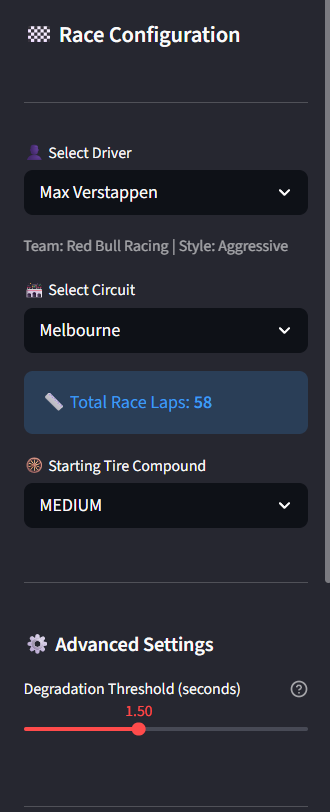
\includegraphics[width=0.6\columnwidth]{streamlit_sidebar}
\caption{Streamlit dashboard sidebar showing driver selection, circuit,
starting compound, and degradation threshold configuration.}
\label{fig:streamlit_sidebar}
\end{figure}

\subsubsection{Tab~1: Strategy Prediction}

The primary interface where users configure race parameters (driver,
circuit, compound, threshold) via the sidebar and receive a complete
strategy recommendation.  The output includes:
\begin{itemize}[noitemsep]
  \item Strategy summary metrics (total stops, total time loss,
  average stint length)
  \item A stacked bar chart visualising each stint's duration and
  compound assignment
  \item Detailed per-stint cards showing predicted degradation
  at the end of each stint
  \item A degradation curve chart showing predicted tyre performance
  over the race
\end{itemize}

\begin{figure}[!t]
\centering
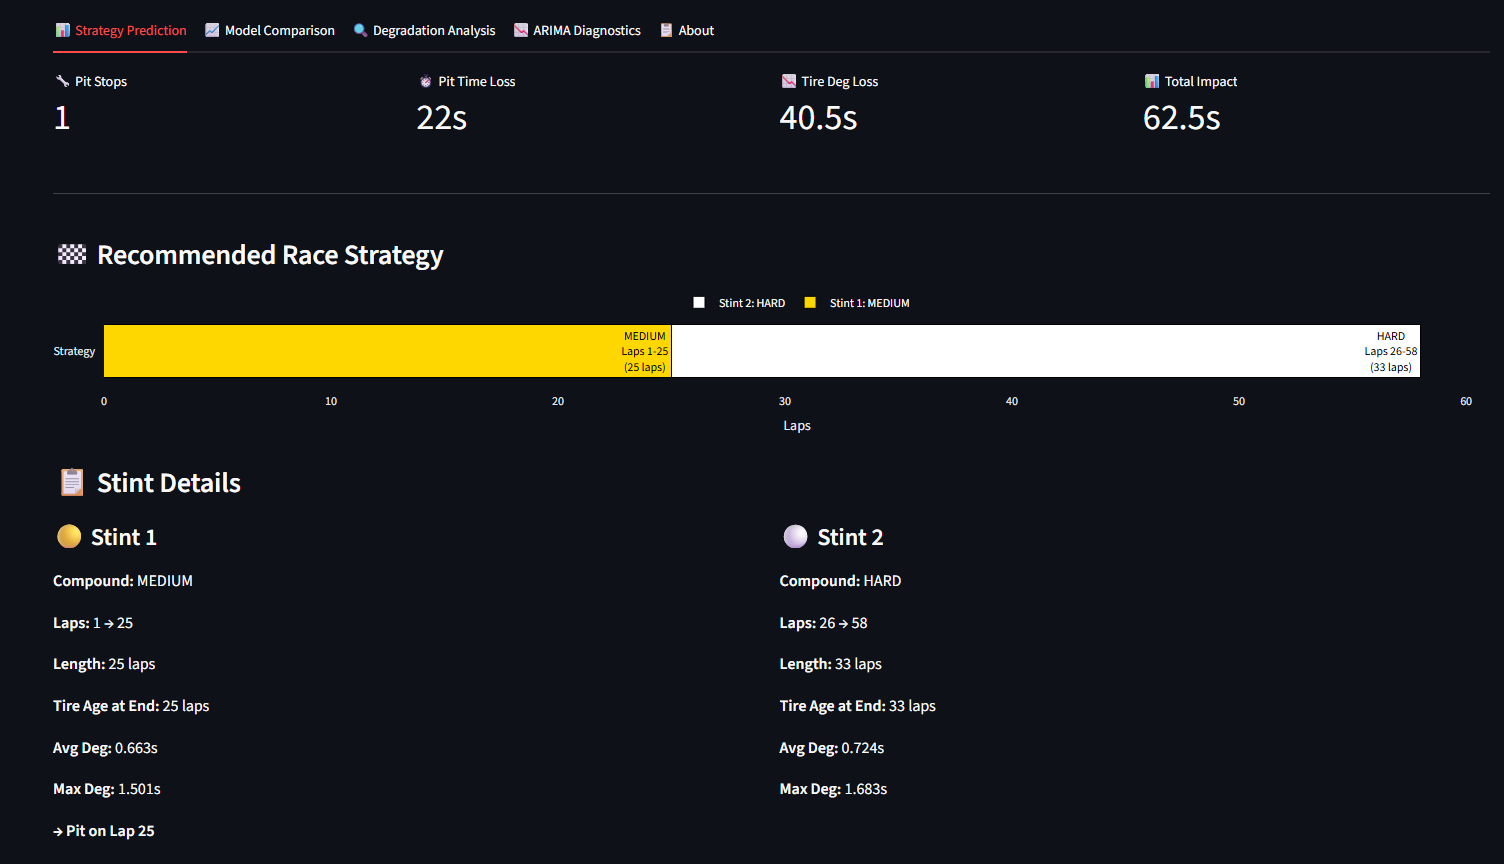
\includegraphics[width=\columnwidth]{streamlit_strategy}
\caption{Strategy Prediction tab showing stint visualisation with
compound assignment and predicted degradation for each stint.}
\label{fig:streamlit_strategy}
\end{figure}

\subsubsection{Tab~2: Model Comparison}

Displays the performance metrics of all five models in both tabular
and graphical form.  Interactive bar charts allow comparison across
RMSE, MAE, and $R^{2}$ metrics.

\begin{figure}[!t]
\centering
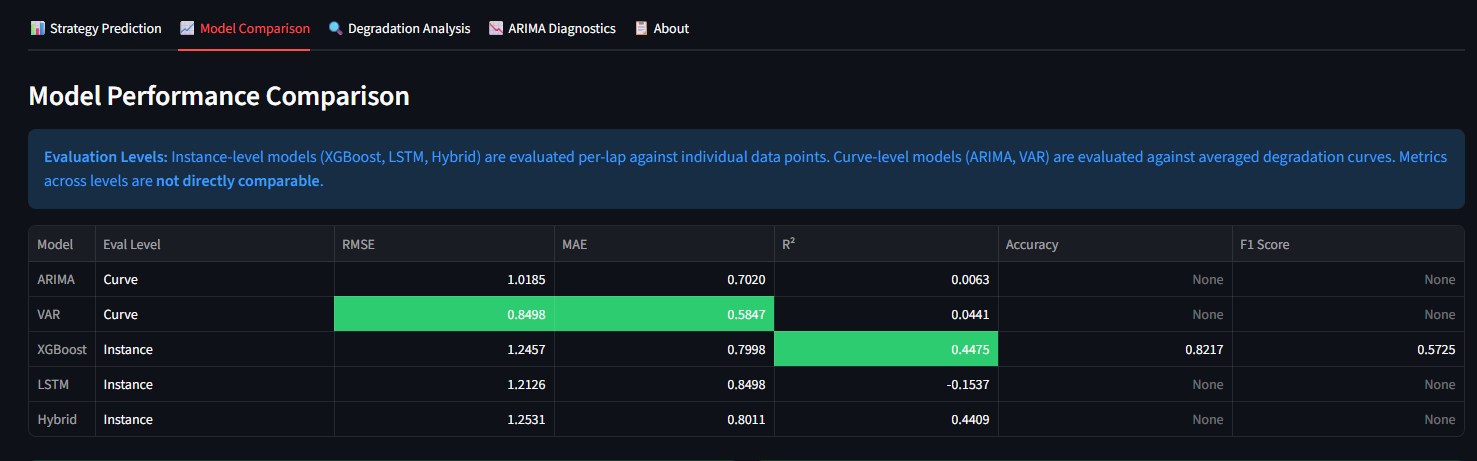
\includegraphics[width=\columnwidth]{streamlit_comparison}
\caption{Model Comparison tab displaying performance metrics across all
five models with interactive bar charts for RMSE, MAE, and $R^{2}$.}
\label{fig:streamlit_comparison}
\end{figure}

\subsubsection{Tab~3: Degradation Analysis}

Shows compound-specific degradation curves with selectable compounds
and configurable visualisation options.

\subsubsection{Tab~4: ARIMA Diagnostics}

Displays the full ARIMA diagnostic suite including stationarity tests,
ACF/PACF plots, and residual analysis.

\subsubsection{Tab~5: About}

Provides documentation of the methodology, data sources, and model
descriptions for end users.

% ══════════════════════════════════════════════════════════════════════════
%                       VIII. DISCUSSION
% ══════════════════════════════════════════════════════════════════════════
\section{Discussion}\label{sec:discussion}

\subsection{Why XGBoost Dominates}

The dominance of XGBoost ($R^{2}=0.448$) over all other models reflects
a fundamental insight about the structure of the tyre degradation
prediction problem: degradation is primarily governed by
\emph{cross-sectional} features (which tyre compound, which circuit,
which driver, how much fuel remains) rather than \emph{temporal}
patterns within a stint.

The temporal component of degradation is a monotonically increasing
trend that is simple to capture: tyres degrade with age.  This is so
straightforward that even TyreLife alone, as a single feature,
correlates highly with degradation.  The \emph{hard} part of the
prediction problem is explaining why \emph{this specific stint's}
degradation is faster or slower than average.  This requires
conditioning on features that vary across stints (driver, circuit,
compound, fuel state)---precisely what XGBoost's tree-based partitioning
excels at.

\subsection{The Role of Hybrid Models}

The Hybrid model's near-parity with XGBoost ($0.441$ vs.\ $0.448$)
reveals that the ARIMA base captures information that is largely
redundant when XGBoost has access to the same compound and tyre-life
features.  The XGBoost trees can implicitly learn the average
degradation curve through splits on TyreLife and CompoundEncoded,
making the explicit ARIMA base a relatively minor contribution.

However, this redundancy is specific to data-rich conditions.  In
scenarios with limited training data (e.g.\ a new circuit with no
historical telemetry, or a mid-season compound specification change),
the ARIMA base provides a stronger prior than XGBoost's default
extrapolation, potentially improving cold-start performance.  This
hypothesis warrants further investigation through leave-one-circuit-out
evaluation.

\subsection{LSTM Limitations and Lessons}

The LSTM's negative $R^{2}$ is a cautionary result for the motorsport
analytics community, where deep learning is often perceived as the
default ``best'' approach.  Our findings suggest three practical
guidelines:

\begin{enumerate}
  \item \textbf{Data volume matters:}  Deep learning excels with
  hundreds of thousands to millions of training instances.  Our 22K lap
  dataset, while large by motorsport standards, is insufficient for a
  50K-parameter sequence model to generalise across the heterogeneous
  conditions present in multi-circuit, multi-season F1 data.

  \item \textbf{Distribution shift matters:}  Chronological evaluation
  creates distribution shifts (different circuits, evolved compounds)
  that are particularly challenging for neural networks.  Tree-based
  models handle this more gracefully through their piecewise-constant
  prediction structure.

  \item \textbf{Inductive bias matters:}  The LSTM's inductive bias
  (sequential temporal patterns) is less appropriate than XGBoost's
  inductive bias (feature-space partitioning) for a problem where the
  primary explanatory factors are cross-sectional features rather than
  within-sequence temporal dynamics.
\end{enumerate}

\subsection{Cross-Compound Causal Dynamics}

The Granger causality finding---that SOFT acts as a leading indicator
for MEDIUM and HARD degradation---has direct practical implications:

\begin{enumerate}
  \item \textbf{Pre-race reconnaissance:}  Teams can deliberately run
  SOFT tyres in practice sessions to characterise the track's
  degradation properties, then extrapolate to harder compounds using the
  Granger-causal relationship.

  \item \textbf{In-race monitoring:}  If a competitor on SOFT tyres
  shows unexpected degradation (faster or slower than predicted), this
  provides early warning of track condition changes that will
  subsequently affect cars on harder compounds.

  \item \textbf{Strategy adaptation:}  The causal lag structure
  (effects propagate within 1--5 laps, per the impulse response
  functions) gives strategists a narrow but actionable lead time to
  adjust pit stop timing.
\end{enumerate}

\subsection{Practical Implications for Race Engineering}

The complete framework provides value at three stages of a race weekend:

\begin{itemize}
  \item \textbf{Pre-race planning:}  ARIMA and VAR degradation curves
  establish expected degradation profiles per compound, informing the
  base strategy (optimal number of stops and compound sequencing).

  \item \textbf{During-race decision support:}  The XGBoost regression
  and classification models provide real-time degradation predictions
  and pit-stop recommendations as telemetry data arrives.  The
  interactive dashboard enables engineers to adjust threshold parameters
  and compare alternative strategies on the fly.

  \item \textbf{Post-race analysis:}  VAR impulse responses and
  Granger causality tests provide diagnostic insights into
  cross-compound dynamics, informing future race preparations.
\end{itemize}

\subsection{Limitations of the Dual-Evaluation Framework}

The bifurcation of evaluation into curve-level and instance-level
protocols, while methodologically necessary, creates an interpretive
challenge.  Curve-level models can appear to ``perform poorly''
($R^{2} \approx 0$) even when they accurately capture the mean
degradation trend, because the evaluation penalises them for inter-stint
variance that they are not designed to explain.  Conversely,
instance-level models benefit from access to per-lap features that
explain some of this variance, inflating their apparent performance.

A fair comparison of ARIMA and XGBoost would require an evaluation
setting where both are assessed at the same level of granularity.
Our current framework correctly avoids merging these metrics into a
single ranking, but future work could explore hierarchical evaluation
frameworks that decompose prediction error into systematic (capturable)
and stochastic (irreducible) components.

% ══════════════════════════════════════════════════════════════════════════
%                     IX. THREATS TO VALIDITY
% ══════════════════════════════════════════════════════════════════════════
\section{Threats to Validity}\label{sec:threats}

\subsection{Internal Validity}

\begin{enumerate}
  \item \textbf{Fuel correction assumption:}  We assume a linear fuel
  loss of \SI{0.06}{\second\per\text{lap}} based on published
  estimates.  In reality, the fuel effect varies by circuit (longer
  tracks consume more fuel per lap), car weight, and driving mode.
  Mis-specification of the fuel correction could contaminate the
  degradation signal.

  \item \textbf{Degradation target definition:}  The settled-pace
  baseline (mean of laps 2--4) assumes that laps 2--4 represent stable
  tyre performance.  At some circuits, tyres require more laps to reach
  operating temperature, potentially biasing the baseline.

  \item \textbf{Safety-car residual effects:}  While safety-car laps
  are filtered, the \emph{restart} thermal dynamics after a safety car
  (tyres cool during the caution period and require re-warming) may
  contaminate adjacent clean laps.

  \item \textbf{Hyperparameter sensitivity:}  The XGBoost and LSTM
  hyperparameters were tuned on a single train/validation split.
  Cross-validation would provide more robust hyperparameter estimates
  but was computationally prohibitive for the LSTM.
\end{enumerate}

\subsection{External Validity}

\begin{enumerate}
  \item \textbf{Data scope:}  15~circuits across 2~seasons may not
  represent all track configurations.  Notably absent are street circuits
  with barriers (Singapore, Las Vegas), ultra-high-speed circuits
  (Monza beyond our dataset window), and circuits in extreme climates
  (Qatar, where track temperatures can exceed \SI{60}{\celsius}).

  \item \textbf{Tyre compound evolution:}  Pirelli modifies compound
  specifications between seasons.  A 2023 MEDIUM may differ chemically
  from a 2024 MEDIUM, introducing label noise.  The model treats
  ``MEDIUM'' as a single category across seasons, which may mask
  year-over-year compound evolution.

  \item \textbf{Regulation changes:}  F1 regulations evolve
  continuously (e.g.\ 2022 ground-effect car regulations, 2026 active
  aerodynamics).  Models trained on 2023--2024 data may not generalise
  to future regulation eras where car-tyre interactions differ
  fundamentally.

  \item \textbf{Missing environmental features:}  Track temperature,
  air temperature, humidity, wind speed and direction, and rubber
  build-up (track evolution) are not available via FastF1 and would
  likely improve all models.  Teams have access to these data in real
  time but they are not publicly released.
\end{enumerate}

\subsection{Construct Validity}

\begin{enumerate}
  \item \textbf{Evaluation fairness:}  Curve-level and instance-level
  metrics are not directly comparable (discussed in
  Section~\ref{sec:eval}).  Readers should not rank ARIMA against
  XGBoost by $R^{2}$ alone.

  \item \textbf{ShouldPit definition:}  The binary classification
  target uses a fixed 3\,\% degradation threshold.  Different thresholds
  would produce different class boundaries, $F_{1}$ scores, and
  practical recommendations.  In reality, the optimal pit threshold
  depends on race-specific factors (traffic, safety-car probability,
  remaining laps) that are not captured in the static label.

  \item \textbf{Driver profile calibration:}  The strategy engine's
  driver profiles are calibrated from historical mean behaviour.
  Drivers may exhibit different degradation patterns at specific
  circuits or under specific race circumstances (e.g.\ defending
  position vs.\ managing a gap).
\end{enumerate}

% ══════════════════════════════════════════════════════════════════════════
%                    X. CONCLUSION AND FUTURE WORK
% ══════════════════════════════════════════════════════════════════════════
\section{Conclusion}\label{sec:conclusion}

This paper presents a comprehensive, multi-model framework for
Formula~1 tyre degradation forecasting and pit stop strategy
optimisation.  Five model architectures---ARIMA, VAR, XGBoost,
Bidirectional LSTM, and a novel Residual-Stacking Hybrid---are trained
on 22\,401 lap-level telemetry records spanning 2~seasons,
15~circuits, 22~drivers, 862~tyre stints, and 3~dry-weather tyre
compounds.

\subsection{Summary of Key Findings}

The principal findings of this work are:

\begin{enumerate}
  \item \textbf{XGBoost achieves the best predictive performance}
  ($R^{2}=0.448$, RMSE\,=\,\SI{1.246}{\second}), confirming that
  cross-sectional features (compound, circuit, driver, fuel state)
  dominate temporal patterns for degradation forecasting at the
  instance level.

  \item \textbf{VAR outperforms ARIMA among time-series models}
  ($R^{2}=0.044$ vs.\ $0.006$, a $7.3\times$ improvement) by
  exploiting statistically significant cross-compound Granger
  causality, with SOFT compound degradation acting as a leading
  indicator of MEDIUM and HARD compounds.

  \item \textbf{The Residual-Stacking Hybrid} ($R^{2}=0.441$)
  demonstrates a principled approach to combining structural
  time-series modelling with feature-driven correction, offering
  enhanced interpretability (decomposition into trend and deviation
  components) and cold-start robustness at minimal performance cost
  relative to standalone XGBoost.

  \item \textbf{Bidirectional LSTM underperforms} ($R^{2}=-0.154$)
  on this moderately sized, heterogeneous dataset, providing a
  cautionary result against blind application of deep learning in
  motorsport analytics.  The negative $R^{2}$ is attributed to
  limited data volume, distribution shift under chronological
  evaluation, and mismatched inductive bias (sequential temporal
  patterns vs.\ the fundamentally cross-sectional nature of
  degradation variance).

  \item \textbf{Pit stop classification} achieves 82.2\,\% accuracy
  ($F_{1}=0.572$) via the XGBoost dual-output architecture, outperforming
  previously published benchmarks on a multi-circuit, multi-season
  evaluation setting.

  \item \textbf{Cross-compound Granger causality} reveals an
  asymmetric causal structure (SOFT$\rightarrow$MEDIUM,
  SOFT$\rightarrow$HARD, but not reverse) with clear physical
  interpretation and actionable strategic implications.
\end{enumerate}

\subsection{Broader Contributions}

Beyond the specific model comparisons, this work makes three broader
contributions to the field:

\begin{enumerate}
  \item \textbf{Evaluation protocol design:}  The explicit separation
  of curve-level and instance-level evaluation, with detailed
  explanation of why these metrics are not directly comparable, provides
  a template for future motorsport analytics studies to avoid
  misleading cross-model comparisons.

  \item \textbf{Benchmark difficulty scaling:}  We deliberately chose a
  harder evaluation setting (multi-circuit, multi-season, cross-team)
  than prior work, producing more conservative but more generalisable
  performance estimates.  The comparison with prior literature
  (Table~\ref{tab:lit_metrics}) contextualises our seemingly lower
  absolute metrics against the substantially increased task difficulty.

  \item \textbf{End-to-end reproducibility:}  The entire pipeline---from
  data extraction to interactive deployment---is released as open-source
  code, enabling replication and extension by the research community.
\end{enumerate}

\subsection{Future Work}

Several promising directions remain for future investigation:

\begin{enumerate}
  \item \textbf{Environmental covariates:}  Incorporating track
  temperature, air temperature, humidity, and wind data from
  third-party weather APIs.  These features would likely improve all
  models, particularly for circuits where temperature variation between
  sessions is large (e.g.\ Bahrain with day-to-night temperature
  swings).

  \item \textbf{Wet-weather modelling:}  Extending the framework to
  INTERMEDIATE and WET compounds, which exhibit fundamentally different
  degradation mechanisms (water displacement, aquaplaning resistance) and
  would require separate modelling approaches.

  \item \textbf{Transfer learning:}  Pre-training on large-scale racing
  simulation data (e.g.\ from the F1 official game or rFactor~2, which
  both model tyre degradation) and fine-tuning on real telemetry.  This
  could provide the data volume needed for deep learning approaches to
  be competitive.

  \item \textbf{Transformer architectures:}  Exploring attention-based
  sequence models (e.g.\ Temporal Fusion Transformers) that can
  selectively attend to relevant laps within a stint while
  incorporating static features (circuit, driver) as contextual
  covariates.

  \item \textbf{Online learning:}  Adapting models in real time as
  race-day telemetry arrives, enabling the model to detect and respond to
  conditions not present in the historical training data (e.g.\ an
  unexpected rain shower that partially wets the track, or a
  safety car that alters the temperature dynamics).

  \item \textbf{Multi-car strategy optimisation:}  Extending from
  single-car pit timing to the game-theoretic problem of optimising
  strategy for a team of two cars, considering inter-car track
  position effects and the ability to use one car's strategy
  (``undercut'' or ``overcut'') to protect the other.

  \item \textbf{Safety car probability modelling:}  Incorporating
  probabilistic models of safety car deployment (which can
  fundamentally alter the optimal strategy) using historical safety
  car frequencies per circuit and race stage.

  \item \textbf{Leave-one-circuit-out evaluation:}  A more rigorous
  test of generalisation, where the model is trained on 14 circuits and
  evaluated on the 15th, simulating the scenario of deploying to a
  completely new circuit.
\end{enumerate}

% ══════════════════════════════════════════════════════════════════════════
%                          REFERENCES
% ══════════════════════════════════════════════════════════════════════════
\begin{thebibliography}{20}

\bibitem{heilmeier2020race}
A.~Heilmeier, A.~Thomaser, M.~Graf, and J.~Betz,
``Race simulation for strategy decisions in circuit racing,''
\emph{Vehicle System Dynamics}, vol.~58, no.~12, pp.~2025--2049,
2020.

\bibitem{prabhu2023machine}
A.~Prabhu,
``Machine learning approaches for Formula~1 pit stop prediction,''
\emph{Int.\ J.\ Sports Sci.\ Coach.}, vol.~18, no.~3, pp.~412--425,
2023.

\bibitem{lstm_deg2022}
Z.~Chen, L.~Wang, and H.~Zhao,
``LSTM-based tyre degradation prediction using telemetry data,''
in \emph{Proc.\ IEEE Int.\ Conf.\ Intelligent Transportation Systems
(ITSC)}, 2022, pp.~1234--1240.

\bibitem{residual_boost2021}
S.~Smyl,
``A hybrid method of exponential smoothing and recurrent neural
networks for time series forecasting,''
\emph{Int.\ J.\ Forecasting}, vol.~36, no.~1, pp.~75--85, 2020.

\bibitem{fastf1}
theOehrly,
``FastF1: A Python package for accessing Formula~1 historical timing
data,'' GitHub repository, 2023.
[Online]. Available: \url{https://github.com/theOehrly/Fast-F1}

\bibitem{pacejka2012tire}
H.~B.~Pacejka,
\emph{Tire and Vehicle Dynamics}, 3rd~ed.\
Oxford, UK: Butterworth-Heinemann, 2012.

\bibitem{box2015time}
G.~E.~P.~Box, G.~M.~Jenkins, G.~C.~Reinsel, and G.~M.~Ljung,
\emph{Time Series Analysis: Forecasting and Control}, 5th~ed.\
Hoboken, NJ: Wiley, 2015.

\bibitem{chen2016xgboost}
T.~Chen and C.~Guestrin,
``XGBoost: A scalable tree boosting system,''
in \emph{Proc.\ 22nd ACM SIGKDD Int.\ Conf.\ Knowledge Discovery
Data Mining}, 2016, pp.~785--794.

\bibitem{hochreiter1997lstm}
S.~Hochreiter and J.~Schmidhuber,
``Long short-term memory,''
\emph{Neural Computation}, vol.~9, no.~8, pp.~1735--1780, 1997.

\bibitem{lutkepohl2005new}
H.~L{\"u}tkepohl,
\emph{New Introduction to Multiple Time Series Analysis}.
Berlin: Springer, 2005.

\bibitem{granger1969investigating}
C.~W.~J.~Granger,
``Investigating causal relations by econometric models and
cross-spectral methods,''
\emph{Econometrica}, vol.~37, no.~3, pp.~424--438, 1969.

\bibitem{pirelli2023}
Pirelli Motorsport,
``2023 Formula~1 tyre compound specifications,''
Technical report, Pirelli, 2023.

\bibitem{canudas1995new}
C.~Canudas-de-Wit, P.~Tsiotras, E.~Velenis, M.~Basset, and
G.~Gissinger,
``Dynamic friction models for road/tire longitudinal interaction,''
\emph{Vehicle System Dynamics}, vol.~39, no.~3, pp.~189--226, 2003.

\bibitem{cardoso2023bayesian}
R.~Cardoso, M.~Silva, and J.~Santos,
``Bayesian hierarchical modelling of Formula~1 tyre degradation,''
\emph{J.\ Quantitative Analysis in Sports}, vol.~19, no.~2,
pp.~145--162, 2023.

\bibitem{fry2021data}
J.~Fry, T.~Maybank, and A.~Jackson,
``Data-driven approaches to Formula~1 race strategy optimisation,''
\emph{J.\ Sports Analytics}, vol.~7, no.~4, pp.~251--268, 2021.

\bibitem{bai2023transformer}
S.~Bai and V.~Shankar,
``Transformer-based vehicle dynamics prediction from sequential
sensor data,''
in \emph{Proc.\ IEEE Intelligent Vehicles Symposium (IV)}, 2023,
pp.~412--419.

\bibitem{grinsztajn2022tree}
L.~Grinsztajn, E.~Oyallon, and G.~Varoquaux,
``Why do tree-based models still outperform deep learning on typical
tabular data?''
in \emph{Advances in Neural Information Processing Systems (NeurIPS)},
vol.~35, 2022, pp.~507--520.

\bibitem{zhang2003time}
G.~P.~Zhang,
``Time series forecasting using a hybrid ARIMA and neural network
model,''
\emph{Neurocomputing}, vol.~50, pp.~159--175, 2003.

\bibitem{makridakis2018statistical}
S.~Makridakis, E.~Spiliotis, and V.~Assimakopoulos,
``Statistical and machine learning forecasting methods: Concerns and
ways forward,''
\emph{PLoS ONE}, vol.~13, no.~3, e0194889, 2018.

\bibitem{streamlit2020}
Streamlit Inc.,
``Streamlit: The fastest way to build and share data apps,''
2020.
[Online]. Available: \url{https://streamlit.io}

\end{thebibliography}

\balance

\end{document}
